\documentclass[11pt,twoside]{article}
\usepackage{amsmath} \usepackage{amssymb} \usepackage{amstext}

% for bibliography:
\usepackage{comment} \usepackage[ backend=biber, ]{biblatex}

\addbibresource{biblio.bib}
% see:
% https://www.sharelatex.com/learn/Bibliography_management_in_LaTeX#The_bibliography_file

\usepackage[export]{adjustbox}

% For corss references 
\usepackage{hyperref} 
%hyperref configuration so that it doesn't contrast so much colorlinks,
\usepackage{xcolor} \hypersetup{ 
linkcolor={red!50!black}, citecolor={blue!50!black}, urlcolor={blue!80!black} }

% Custom Math operators (functions not in italic in math mode):
\DeclareMathOperator{\arcsec}{arcsec} \DeclareMathOperator{\arccot}{arccot}
\DeclareMathOperator{\arccsc}{arccsc} \DeclareMathOperator{\cis}{cis}

\usepackage[spanish]{babel} \usepackage[utf8]{inputenc}
\usepackage[T1]{fontenc}
\usepackage{csquotes}

\usepackage{array} \usepackage{tabularx,colortbl} \usepackage{float}
\usepackage{listings} \usepackage{color} \usepackage{booktabs}
\usepackage{multirow}

\usepackage[framemethod=tikz]{mdframed} \usepackage{amsthm}

%Subfigures
\usepackage{subcaption} \usepackage{relsize} %Bigger math with mathlarger{___}

\definecolor{codegreen}{rgb}{0,0.6,0} \definecolor{codegray}{rgb}{0.5,0.5,0.5}
\definecolor{codepurple}{rgb}{0.58,0,0.82}
\definecolor{backcolour}{rgb}{0.95,0.95,0.92}

\lstdefinestyle{mystyle}{ backgroundcolor=\color{backcolour},
    commentstyle=\color{codegreen}, keywordstyle=\color{blue},
    numberstyle=\tiny\color{codegray}, stringstyle=\color{red},
    identifierstyle=\color{black}, basicstyle=\footnotesize,
    %breakatwhitespace=false,         
    breaklines=true,                 
    %captionpos=b,                    keepspaces=true,                 
    numbers=left,                    numbersep=5pt,
    showspaces=false,                
    %showstringspaces=false, showtabs=false,                  
    tabsize=4 }

\lstset{style=mystyle}


\usepackage[utf8]{inputenc} \usepackage[a4paper, margin=2.5cm, top=3.5cm,
bottom=1in]{geometry}

\renewcommand{\figurename}{Fig.} \renewcommand{\tablename}{Tabla}

\definecolor{lightblue}{RGB}{135,206,250}

\title{ Monografía de Física: \\ Estudio de la forma de salpicaduras formadas
por gotas de agua en función de la altitud y el ángulo de impacto en una
superficie} \author{ Aleix Boné \\ \\ Tutor: Jordi Mazón } \date{\today}

\setcounter{page}{-1}

\includeonly{tables}

\begin{document} \topskip3cm \clearpage\maketitle \thispagestyle{empty}
\vspace{1cm}
    %\footnotetext{Source:
%\url{https://commons.wikimedia.org/wiki/File\%3ADCT-8x8.png} By Devcore (Own
%work) [Public domain], via Wikimedia Commons} \begin{center}
%\begin{figure}[ht] \caption{} \centerline{
                %%\includegraphics[width=0.65\textwidth]{src/DCT-8x8.png}
            %} \end{figure} \end{center}

    \pagebreak \thispagestyle{empty} \topskip0pt 
    \tableofcontents \pagebreak \listoffigures \pagebreak \listoftables \pagebreak
    \section{Resumen} \label{sec:resumen}

\section{Introducción teórica} \label{sec:introduccion_teorica}
%Una gota de líquido al caer desde cierta altura e impactar con un sólido sufre
%un cambio de momento que provoca una deformación de la gota. Esta deformación
%es

\section{Diseño experimental 1} \label{sec:Diseño experimental 1}
\subsection{Objetivo} \label{sub:objetivo} 
El objetivo de este experimento es
determinar la relación entre la altura de caída de una gota de agua y la mancha
que esta genera después de impactar contra una superficie plana.

\subsection{Montaje} \label{sub:montaje} El montaje del experimento consistía
en una lámina de papel de formato DinA4, de densidad $100g/cm^2$ y grosor de
$0.010\ mm$ usada como superficie de impacto y un nivel al que se le añadió una
cinta con medidas asó como un soporte que sujetaba una pipeta Pasteur y que
permitía soltar las gotas con la pipeta Pasteur desde diferentes alturas sobre
la lámina de papel.  Se uso una lámina de papel para cada una de las diferentes
alturas que iban de $10\ cm$ a $100\ cm$ en un incremento de $10\ cm$. Para
recolectar los datos se usó una cámara con la que se fotografiaron las
distintas láminas de papel, las imágenes se tomaron con los mismos valores de
zoom, apertura, velocidad, enfoque e ISO para facilitar el posterior
procesamiento de las imágenes. La cámara se colocó con un trípode apuntando
perpendicularmente a las láminas para eliminar la perspectiva. Cada foto
realizada tenia como referencia una regla al lado de la lámina para determinar
las dimensiones de las manchas en el momento de procesarlas. La figura
\ref{fig:montaje} muestra el montaje experimental.  Se uso agua destilada
mezclada con colorante amarillo para poder procesar las imágenes obtenidas.

\begin{figure}[htpb] \centering
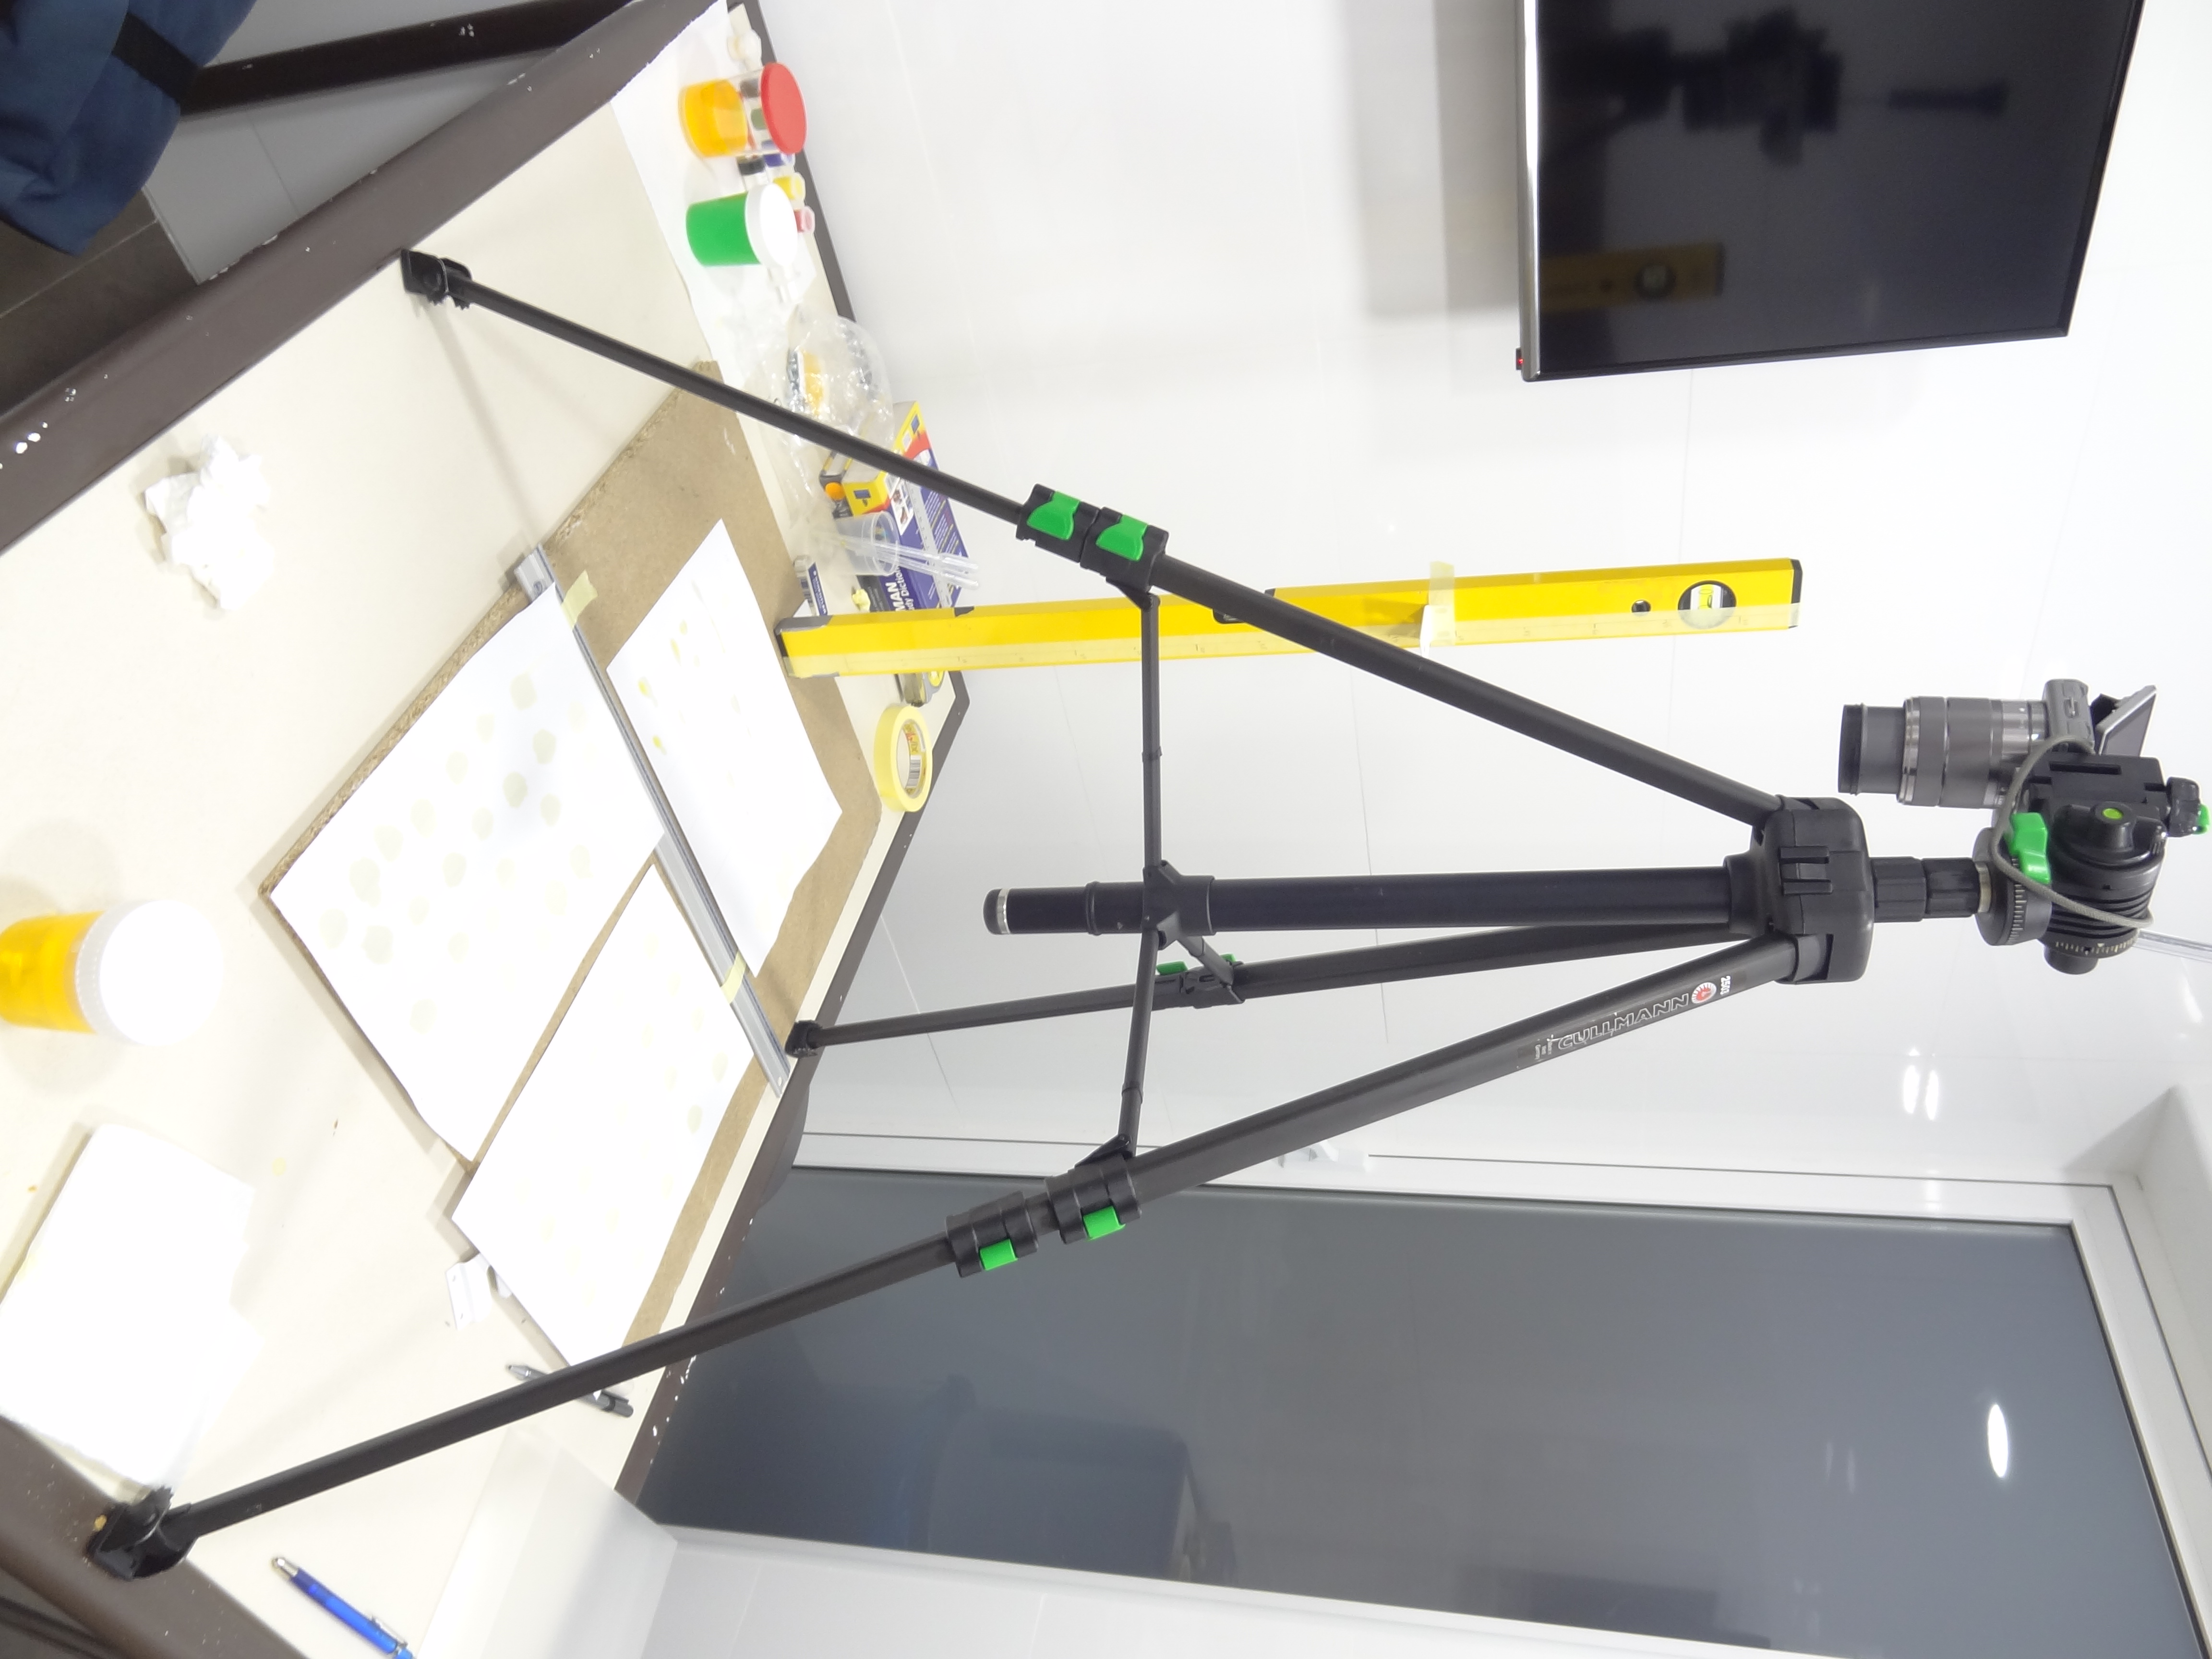
\includegraphics[width=0.8\linewidth,angle=90]{src/montaje.jpg}
\caption{Montaje experimental} \label{fig:montaje} \end{figure}

\subsection{Control de variables} \label{sub:control_de_variables} En este
experimento, la variable independiente es la altura de la que cae la gota de
agua y las variables dependientes son el área de la mancha formada, el
perímetro y el radio que se medirán con un programa informático a partir de las
imágenes capturadas. Para garantizar el mínimo error, se deben controlar las
variables que pueden afectar a las anteriores.  Uno de los puntos más
importantes es las propiedades del líquido en cuestión, puesto que al ser
lanzado con una pipeta Pasteur, el volumen de líquido depende de la tensión
superficial del líquido como muestra la ecuación \ref{eq:pendant_drop} que se
obtiene igualando la fuerza de la gravedad con la fuerza debido a la tensión
superficial de una gota de masa $m$ y tensión superficial $\gamma$ en un tubo
de diámetro $d$ \cite{pendant_drop}.  \begin{align}\label{eq:pendant_drop}
    F_\gamma&=\pi d \gamma \qquad F_\gamma = F_g = mg \nonumber\\ mg &= \pi d
\gamma \nonumber\\ m &= \frac{\pi d \gamma}{g} \end{align} La tensión
superficial de una gota de agua en contacto con vapor de agua puro
\cite{water_tension2} se determina a partir de la ecuación
\ref{eq:water_tension} donde $T$ es la temperatura en grados kelvin.
\begin{equation}\label{eq:water_tension} \gamma_w = 235.8\left(
    1-\frac{T}{697.098} \right)^{1.256} \left[ 1- 0.625\left(
1-\frac{T}{697.098} \right)\right] \frac{\rm mN}{\rm m} \end{equation} Aunque
la ecuación \ref{eq:water_tension} no sea aplicable a nuestro experimento
puesto que solo es válida para agua pura en contacto con vapor de agua pura,
ilustra como la tensión superficial depende de la temperatura. Para controlar
la temperatura e intentar garantizar que la tensión superficial y por
consiguiente el volumen de cada gota lanzada sea constante, los experimentos se
realizaron en un entorno cerrado y se controlaron los cambios de temperatura
con un termómetro (La temperatura se mantuvo oscilando entre los $26.7$ y
$26.8$ grados centígrados durante los experimentos). Se usó siempre la misma
solución de agua destilada con colorante para no alterar las propiedades del
líquido así como el mismo tipo de papel.

\section{Diseño experimental 2} \label{sec:Diseño experimental 2}
\subsection{Objetivo} \label{sub:objetivo2} El objetivo del segundo experimento
es determinar la relación entre el angulo de inclinación de una superficie y la
forma de la mancha generada por una gota que cae sobre esta.

\subsection{Montaje} \label{sub:montaje2} El montaje del segundo experimento es
idéntico al del primer experimento (sección \ref{sub:montaje}) con la
diferencia de que se usó un soporte vertical para inclinar las láminas de papel
diferentes grados. Para determinar la inclinación se usaron cálculos
matemáticos para determinar a que altura se debía fijar el papel en el soporte
vertical para que este tuviera la inclinación deseada, adicionalmente, se
comprobaron los cálculos con un porta ángulos para verificar que la inclinación
era la correcta. La figura \ref{fig:montaje2} Otra de las diferencias es que se
usó un segundo soporte a parte del nivel usado en el experimento 1 que fue
usado en conjunto con el nivel poniendo uno a cada lado de la lámina de papel y
con una regla de $40\ cm$ se unieron para poder poner la pipeta Pasteur con su
soporte en la regla justo encima de la hoja y moverla a la misma altura. Debido
a la inclinación de la lámina se tuvo que calcular para cada hilera de gotas en
la hoja a que altura se debía poner dicha regla para que la gota estuviera
justo a $50\ cm$ de la lámina, que fue la altura usada para todas las medidas
de este experimento.  \begin{figure}[htpb] \centering
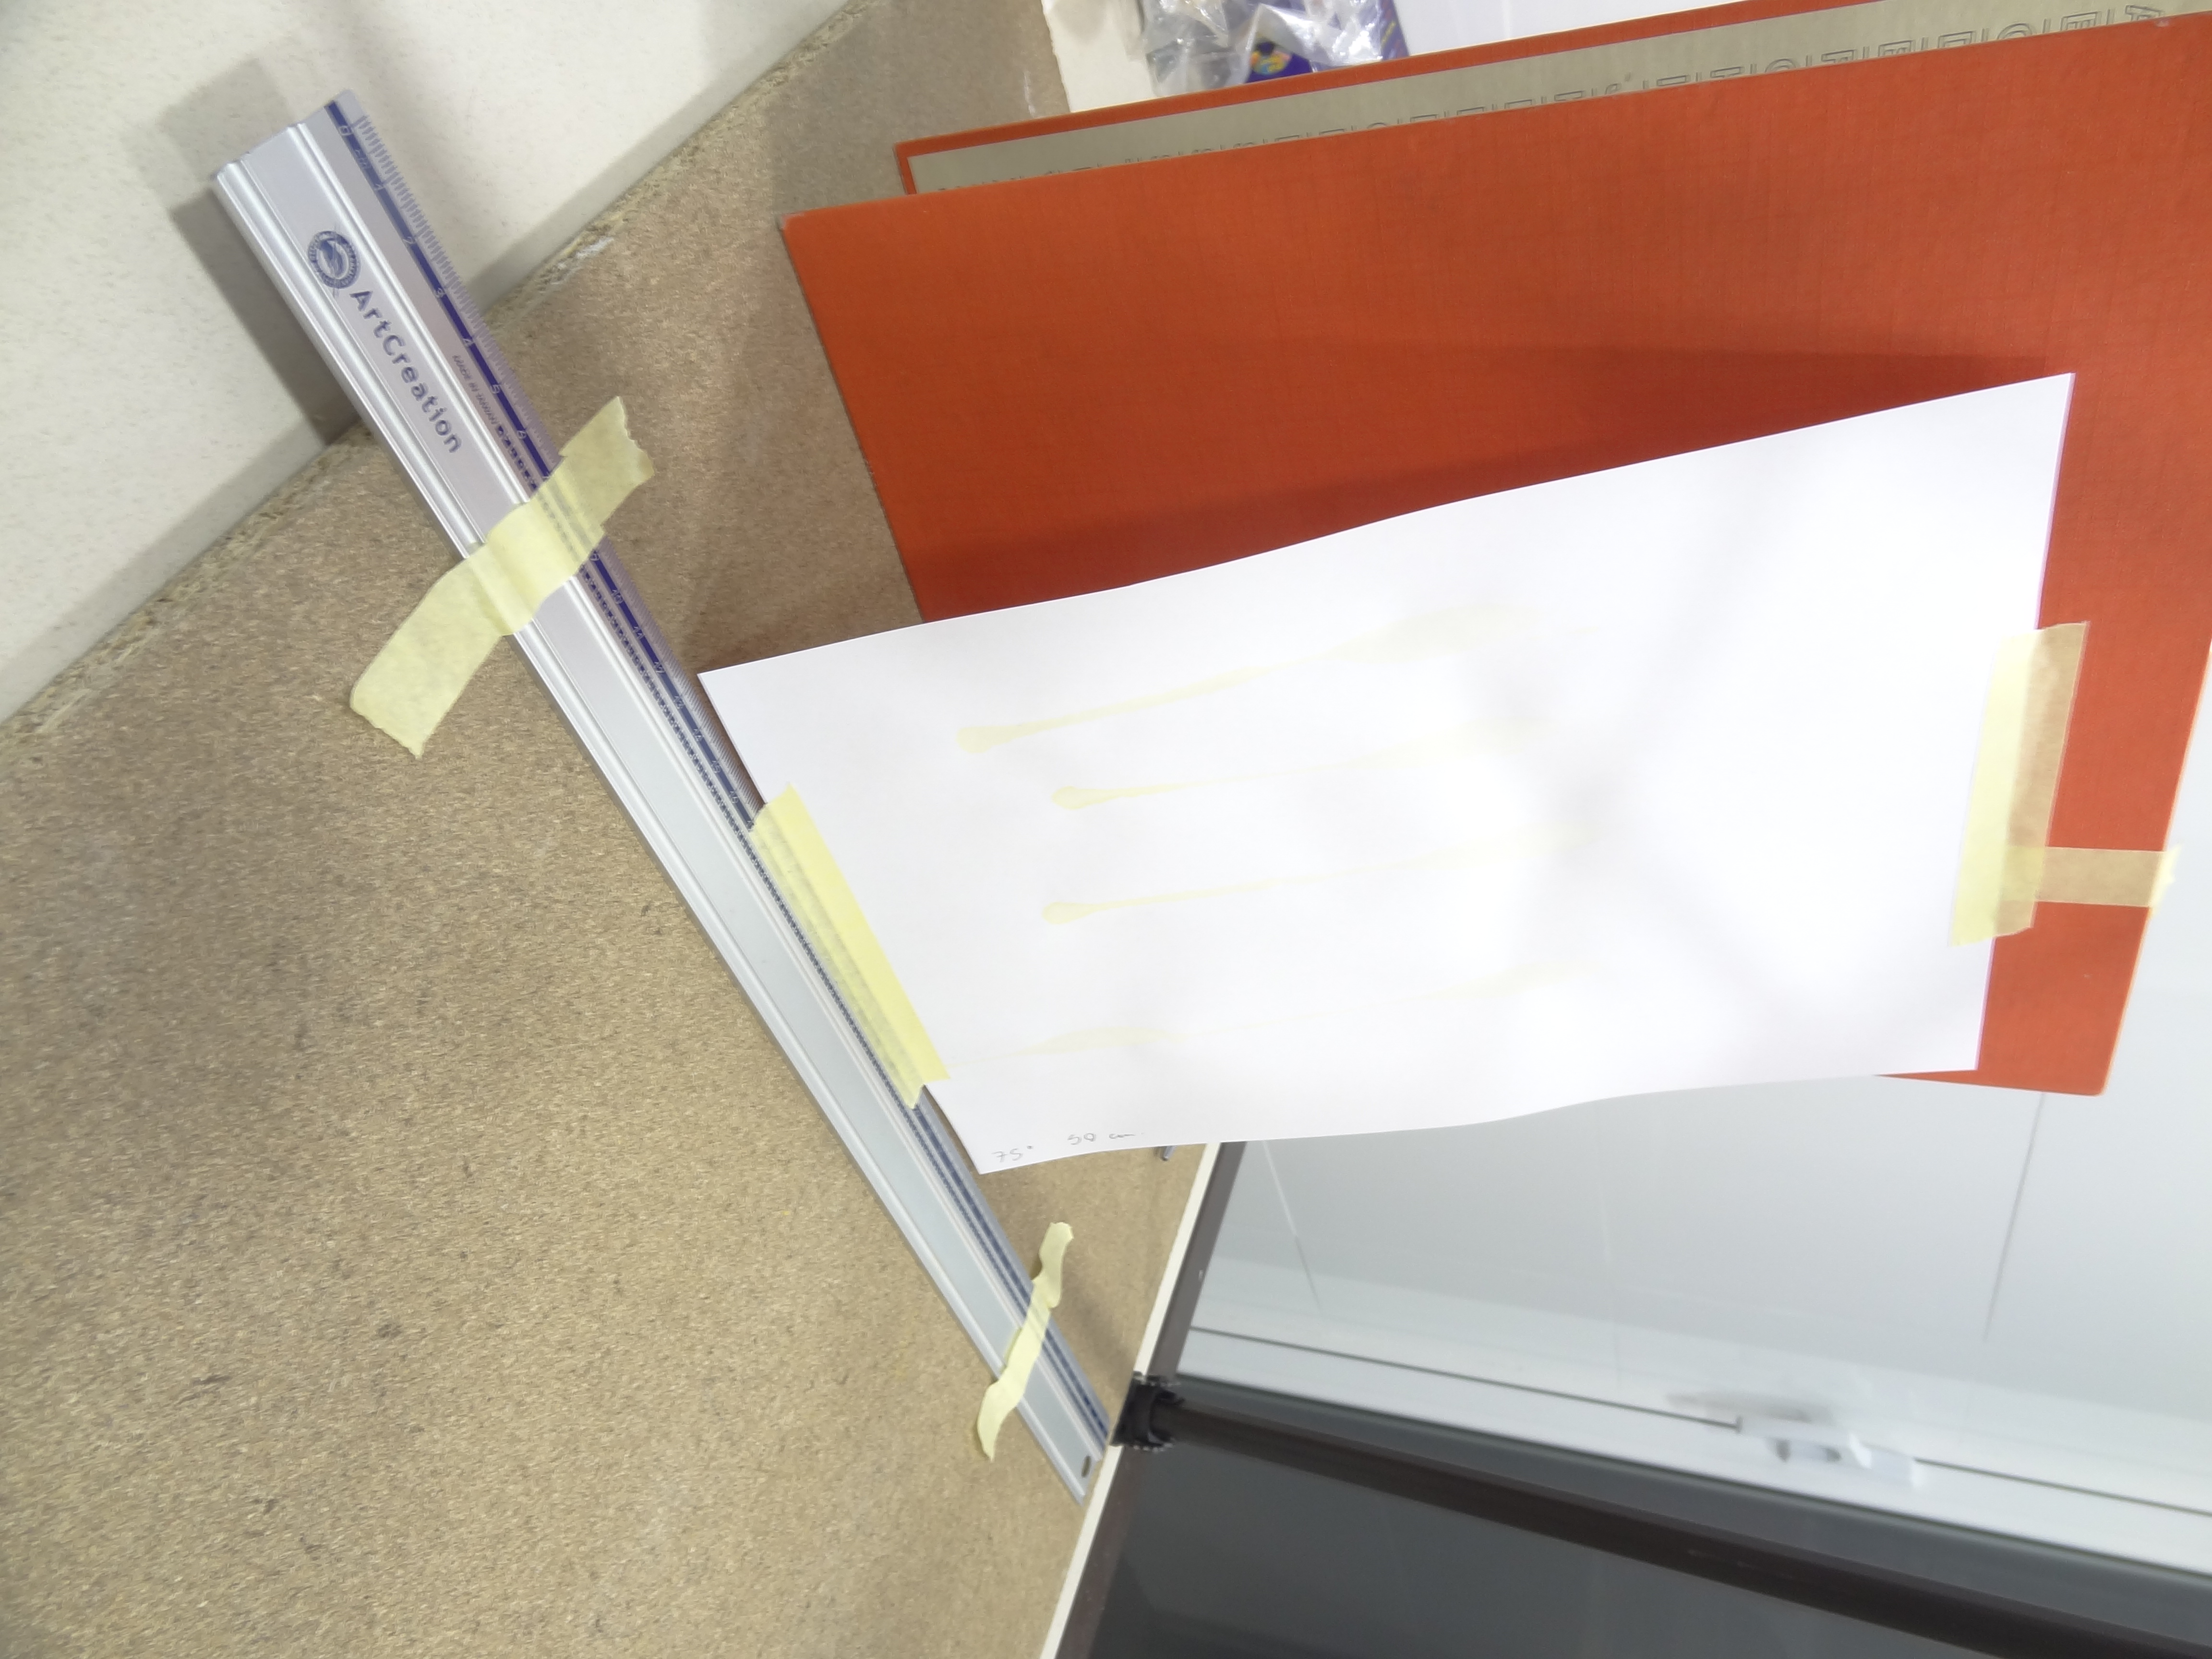
\includegraphics[width=0.8\linewidth,angle=90]{src/montaje2.jpg}
\caption{Montaje experimental con lámina inclinada $75^o$ respecto la
horizontal} \label{fig:montaje2} \end{figure}

\subsection{Control de variables} \label{sub:control_de_variables2} La variable
independiente en este caso es la inclinación del plano y la dependiente la
forma de la mancha formada por la gota, que en este caso esta determinada por
el área, el perímetro, el eje mayor y el eje menor. Al igual que el experimento
anterior, la temperatura es una de las variables que se deben controlar ya que
esta afecta al volumen de agua que habrá en cada gota que caiga de la pipeta de
Pasteur. El experimento se realizó en las mismas condiciones que el anterior, y
la temperatura en este caso varió entre los $25.3^o$ y los $25.6^o$ grados
Celsius (El experimento se realizó unas horas después que el primero). La
altura de la caída se mantuvo constante calculando trigonométricamente la
altura desde la superficie donde se apoyaban los soportes para que la gota
cayera siempre desde $50\ cm$ tal y como se ha mencionado en la sección
\ref{sub:montaje2}.

\pagebreak \section{Datos brutos} \label{sec:datos_brutos} Las imágenes
obtenidas a partir de los experimentos fueron procesadas usando un programa
especializado llamado ImageJ \cite{imagej}. Este programa permite importar
imágenes como la que se muestra en la figura \ref{fig:80img} y definir la
proporción entre pixels y centímetros de la imagen a partir de la regla que
aparece en esta y aislar la forma de las gotas a partir de los diferentes
canales\footnote{Se filtraron las formas usando los siguientes parámetros en el
espacio de color HSL: Matiz[26-54], Saturación[6-255] y Luz[50-255]}.
Obteniendo la imagen que se muestra en la figura \ref{fig:80proc}.  Una vez
procesada la imagen tal como se muestra en la figura \ref{fig:80proc}, el
programa permite ejecutar un algoritmo de cálculo que aisla las regiones
contiguas de color negro, que en nuestra muestra corresponden a la forma de las
gotas y calcular el área negra de cada región así como el perímetro (sin
considerar los agujeros que pueden haber en el interior de la región) y
calcular el eje mayor y menor de la elipse que mejor se adapte a la figura así
como la inclinación de los ejes respecto a la horizontal de la imagen.

Siguen los datos obtenidos por el programa así como las imágenes procesadas con
la escala en la esquina inferior derecha.

\begin{figure}[htpb] \centering
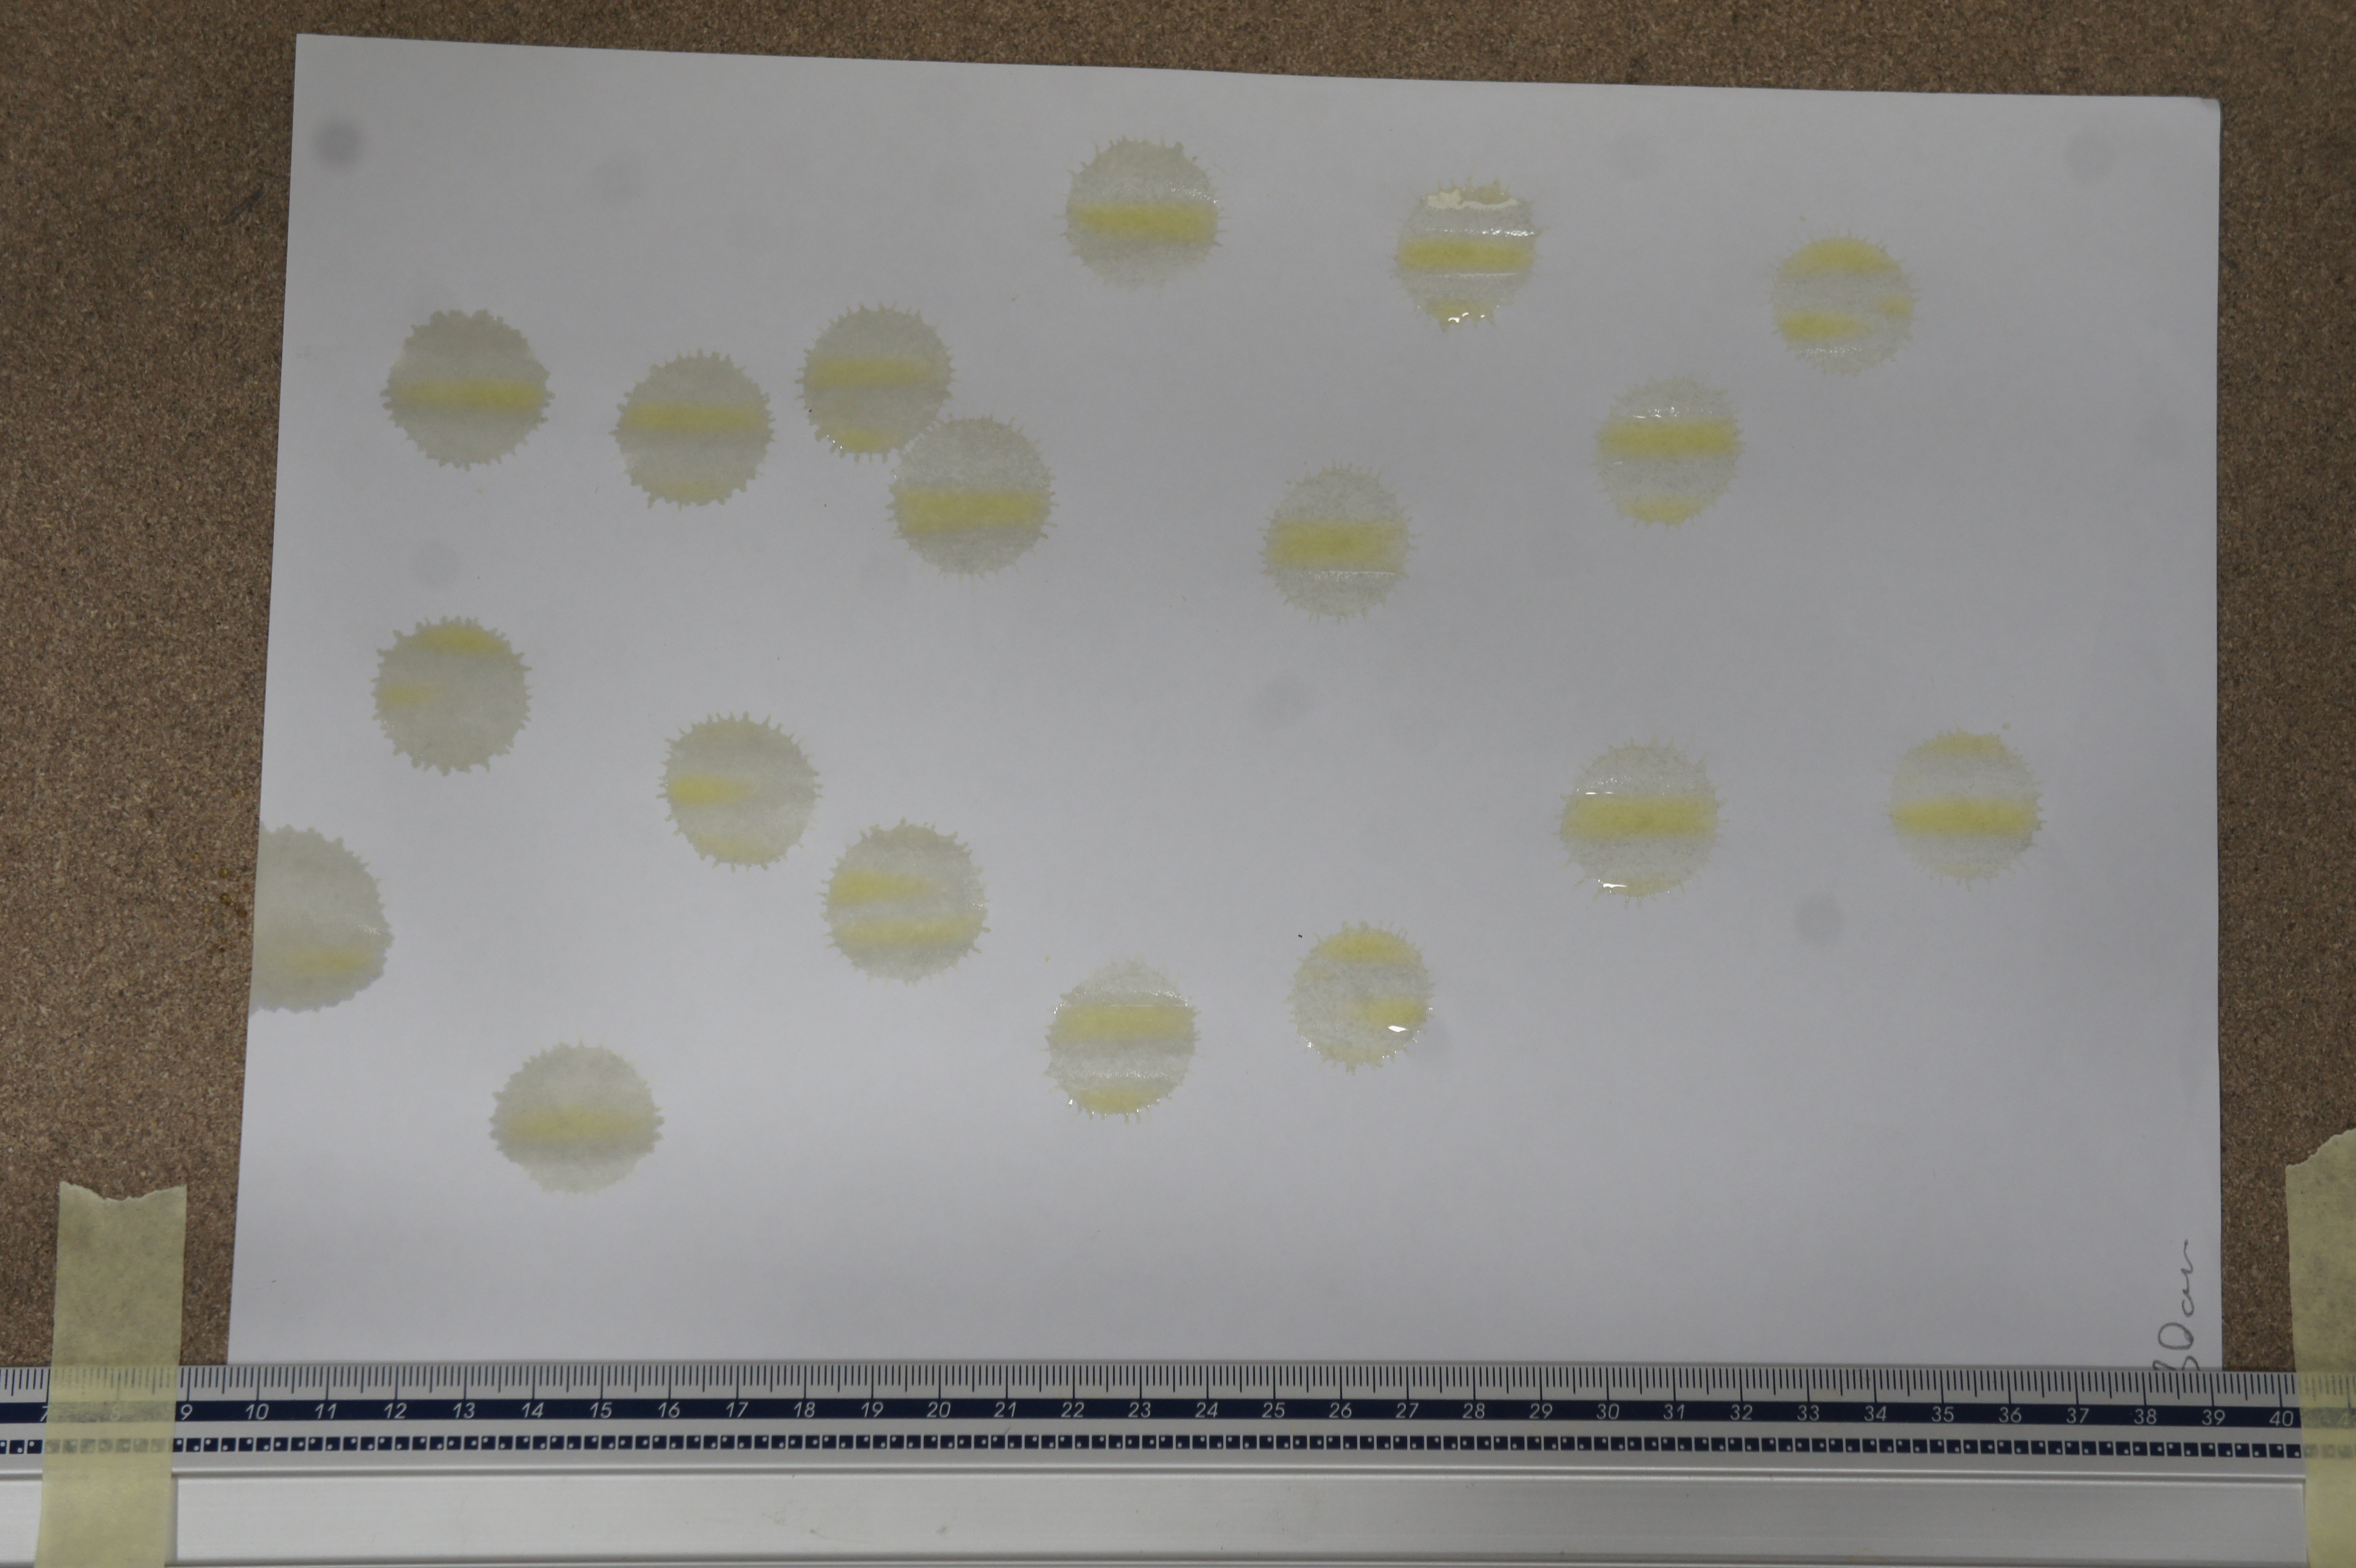
\includegraphics[width=0.60\linewidth]{src/80.JPG} \caption{Imagen original de
manchas lanzadas desde $80\ cm$} \label{fig:80img} \end{figure}
\begin{figure}[htpb] \centering
    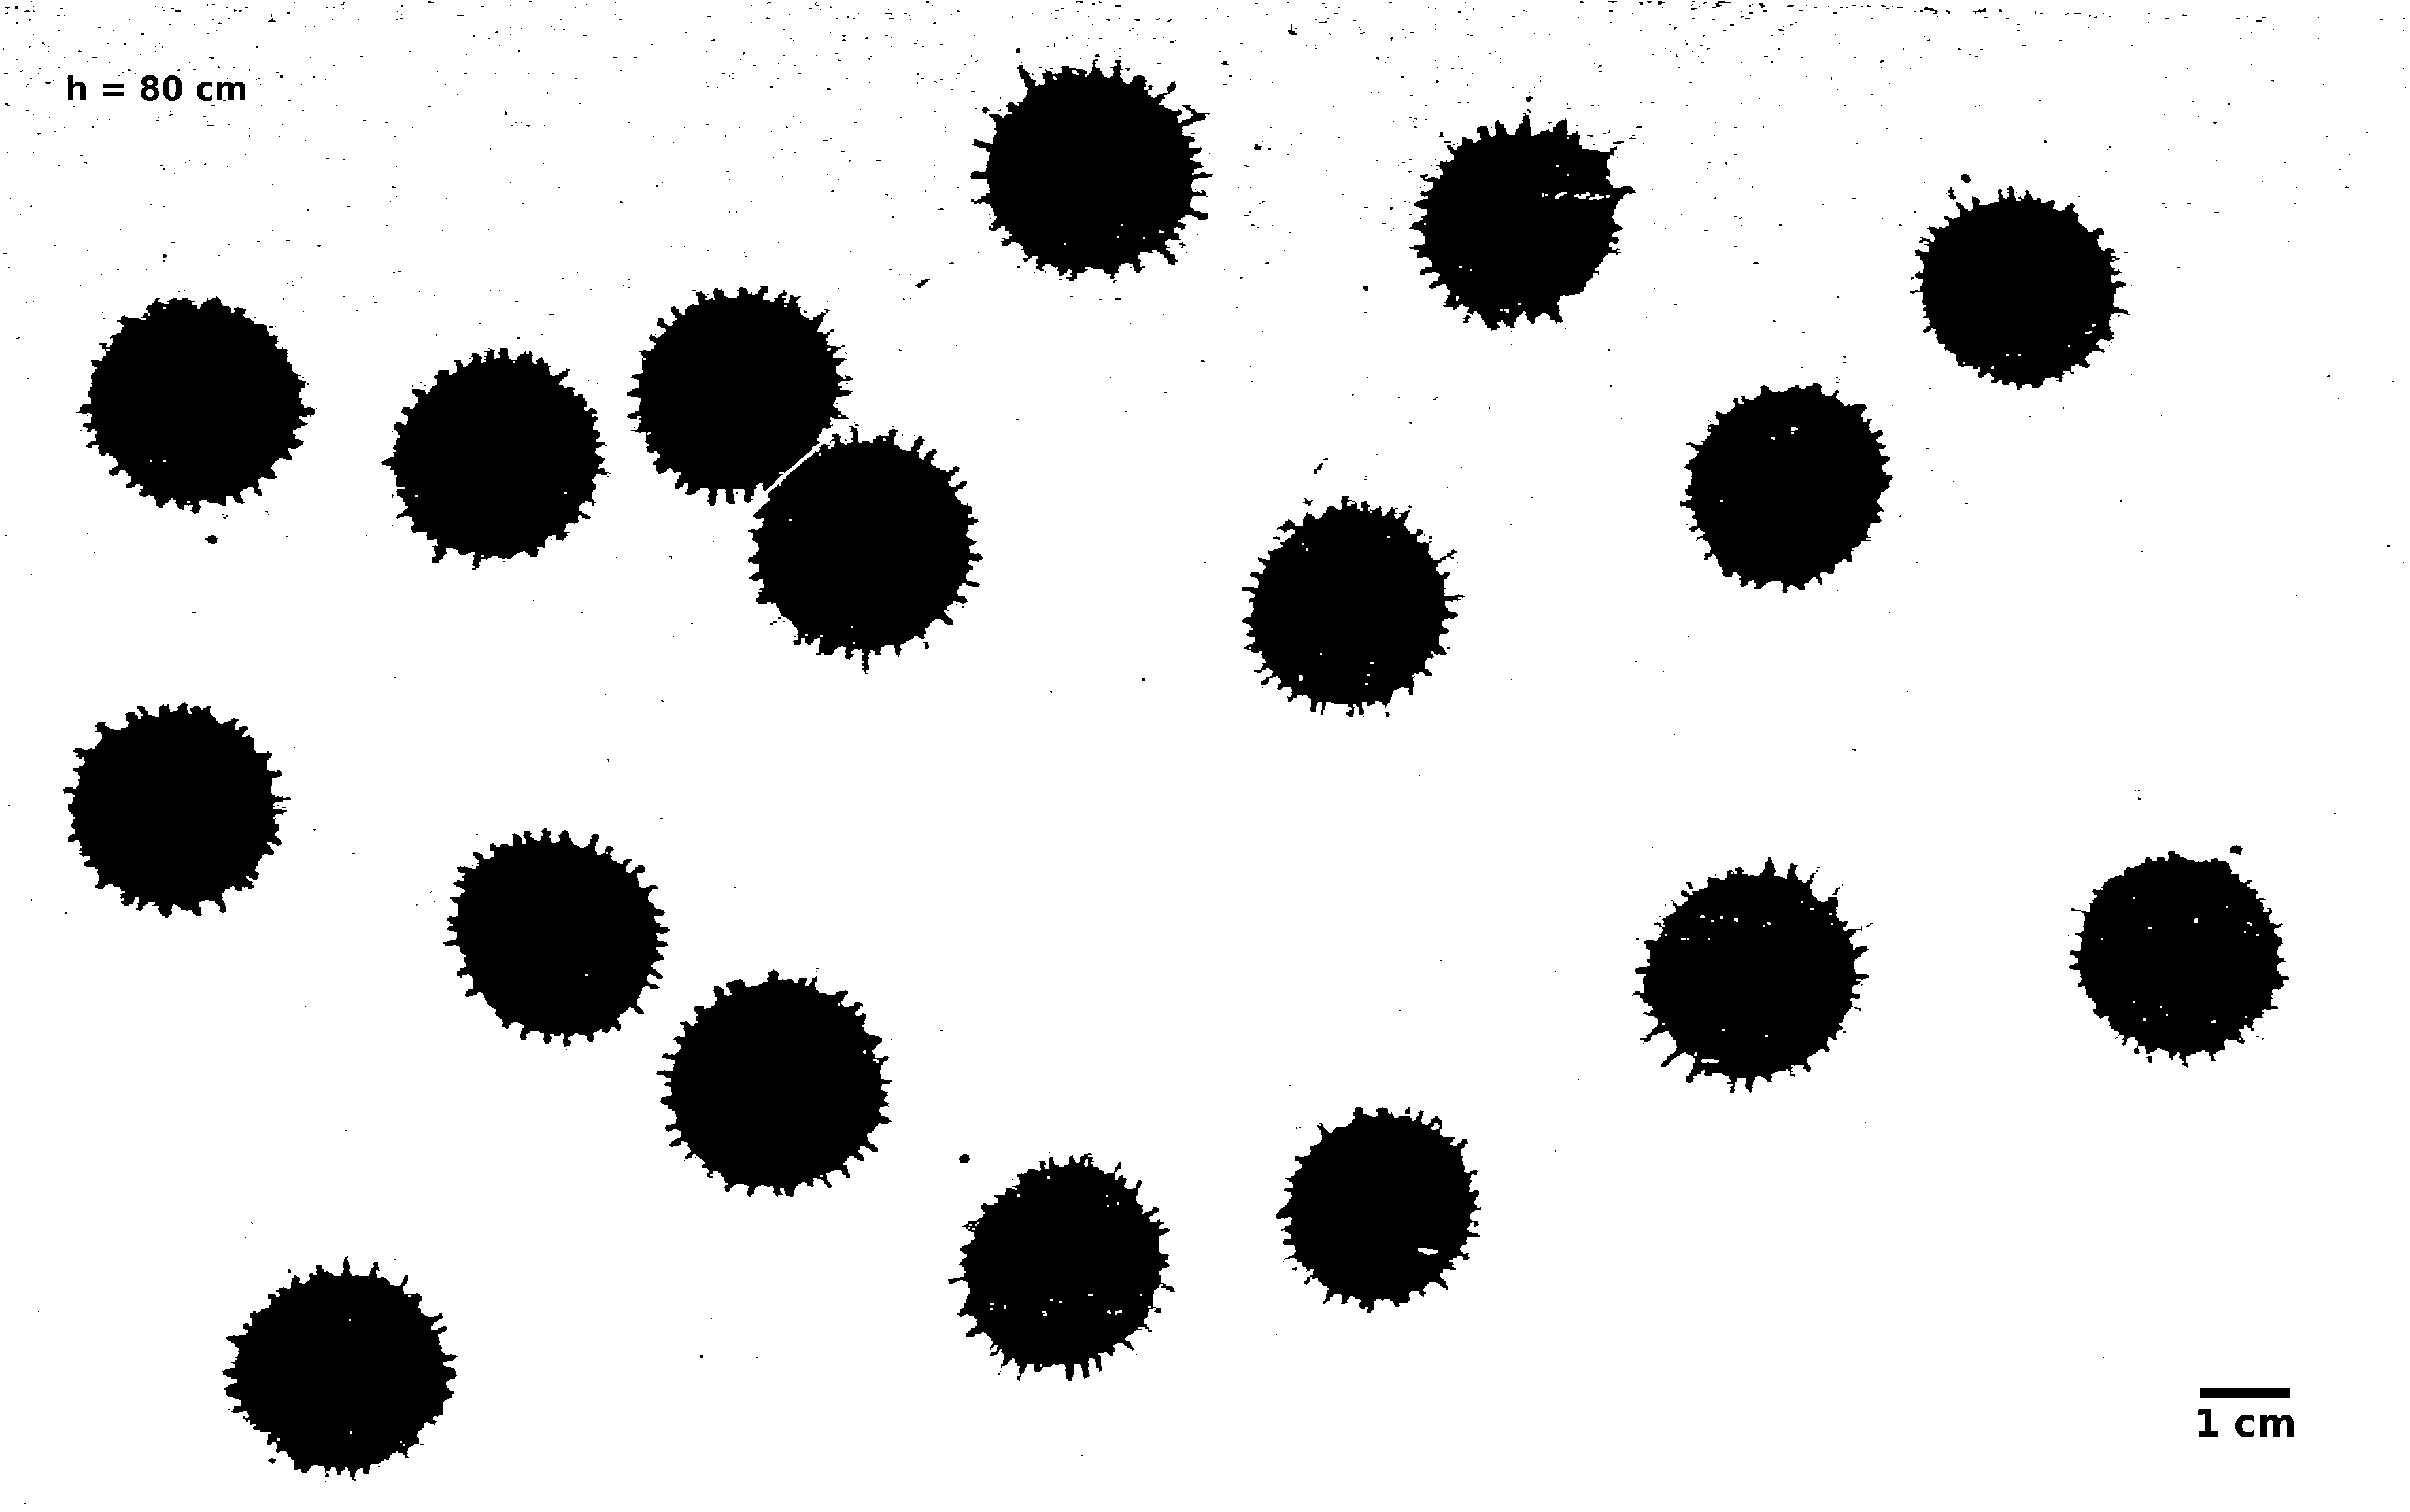
\includegraphics[width=0.60\linewidth]{src/80.png} \caption{Imagen de la
figura \ref{fig:80img} procesada} \label{fig:80proc} \end{figure}

\subsection{Experimento 1} \label{sub:experimento_1}

\begin{table}[H] \centering \caption{Datos obtenidos a partir de la figura
    ~\ref{fig:10cm-1} ($h=10\ cm)$} \label{tab:10cm} \begin{tabular}{cccccc}
        \toprule Gota & Área ($cm^2$) & Perímetro ($cm$) & Eje mayor ($cm$) &
        Eje menor ($cm$) & Dirección ($^o$) \\ \midrule 1     & 2.35 & 10.79 &
        1.76 & 1.70 & 146.39 \\ 2     & 1.73 & 7.66  & 1.51 & 1.45 & 7.69   \\
        3     & 1.82 & 7.93  & 1.56 & 1.49 & 169.17 \\ 4     & 1.19 & 6.22  &
        1.26 & 1.20 & 177.35 \\ 5     & 2.16 & 8.30  & 1.69 & 1.63 & 165.92 \\
        6     & 1.28 & 6.61  & 1.32 & 1.24 & 179.71 \\ 7     & 1.82 & 7.71  &
        1.55 & 1.49 & 161.79 \\ 8     & 1.85 & 8.35  & 1.58 & 1.48 & 176.50 \\
        9     & 1.25 & 6.59  & 1.29 & 1.23 & 172.78 \\ 10    & 1.10 & 5.90  &
        1.22 & 1.15 & 4.08   \\ 11    & 1.56 & 6.58  & 1.44 & 1.38 & 172.67 \\
        12    & 1.68 & 7.96  & 1.50 & 1.42 & 167.94 \\ 13    & 1.69 & 7.26  &
        1.50 & 1.44 & 162.53 \\ 14    & 1.86 & 8.07  & 1.62 & 1.46 & 5.33   \\
        15    & 1.43 & 6.24  & 1.37 & 1.33 & 156.64 \\ 16    & 1.29 & 5.58  &
        1.36 & 1.20 & 1.79   \\ 17    & 1.39 & 6.63  & 1.43 & 1.24 & 173.26 \\
        18    & 1.01 & 4.92  & 1.14 & 1.13 & 38.90  \\ 19    & 1.63 & 7.27  &
        1.48 & 1.41 & 55.99  \\ 20    & 1.38 & 5.98  & 1.37 & 1.28 & 169.43 \\
        21    & 1.65 & 6.59  & 1.49 & 1.41 & 171.47 \\ 22    & 1.69 & 7.00  &
        1.53 & 1.40 & 116.89 \\ 23    & 1.65 & 8.01  & 1.55 & 1.36 & 86.05  \\
    \midrule Media & 1.59 & 7.14  & 1.46 & 1.37 & 123.49 \\ \bottomrule
\end{tabular} \end{table}

\begin{figure}[H] \centering
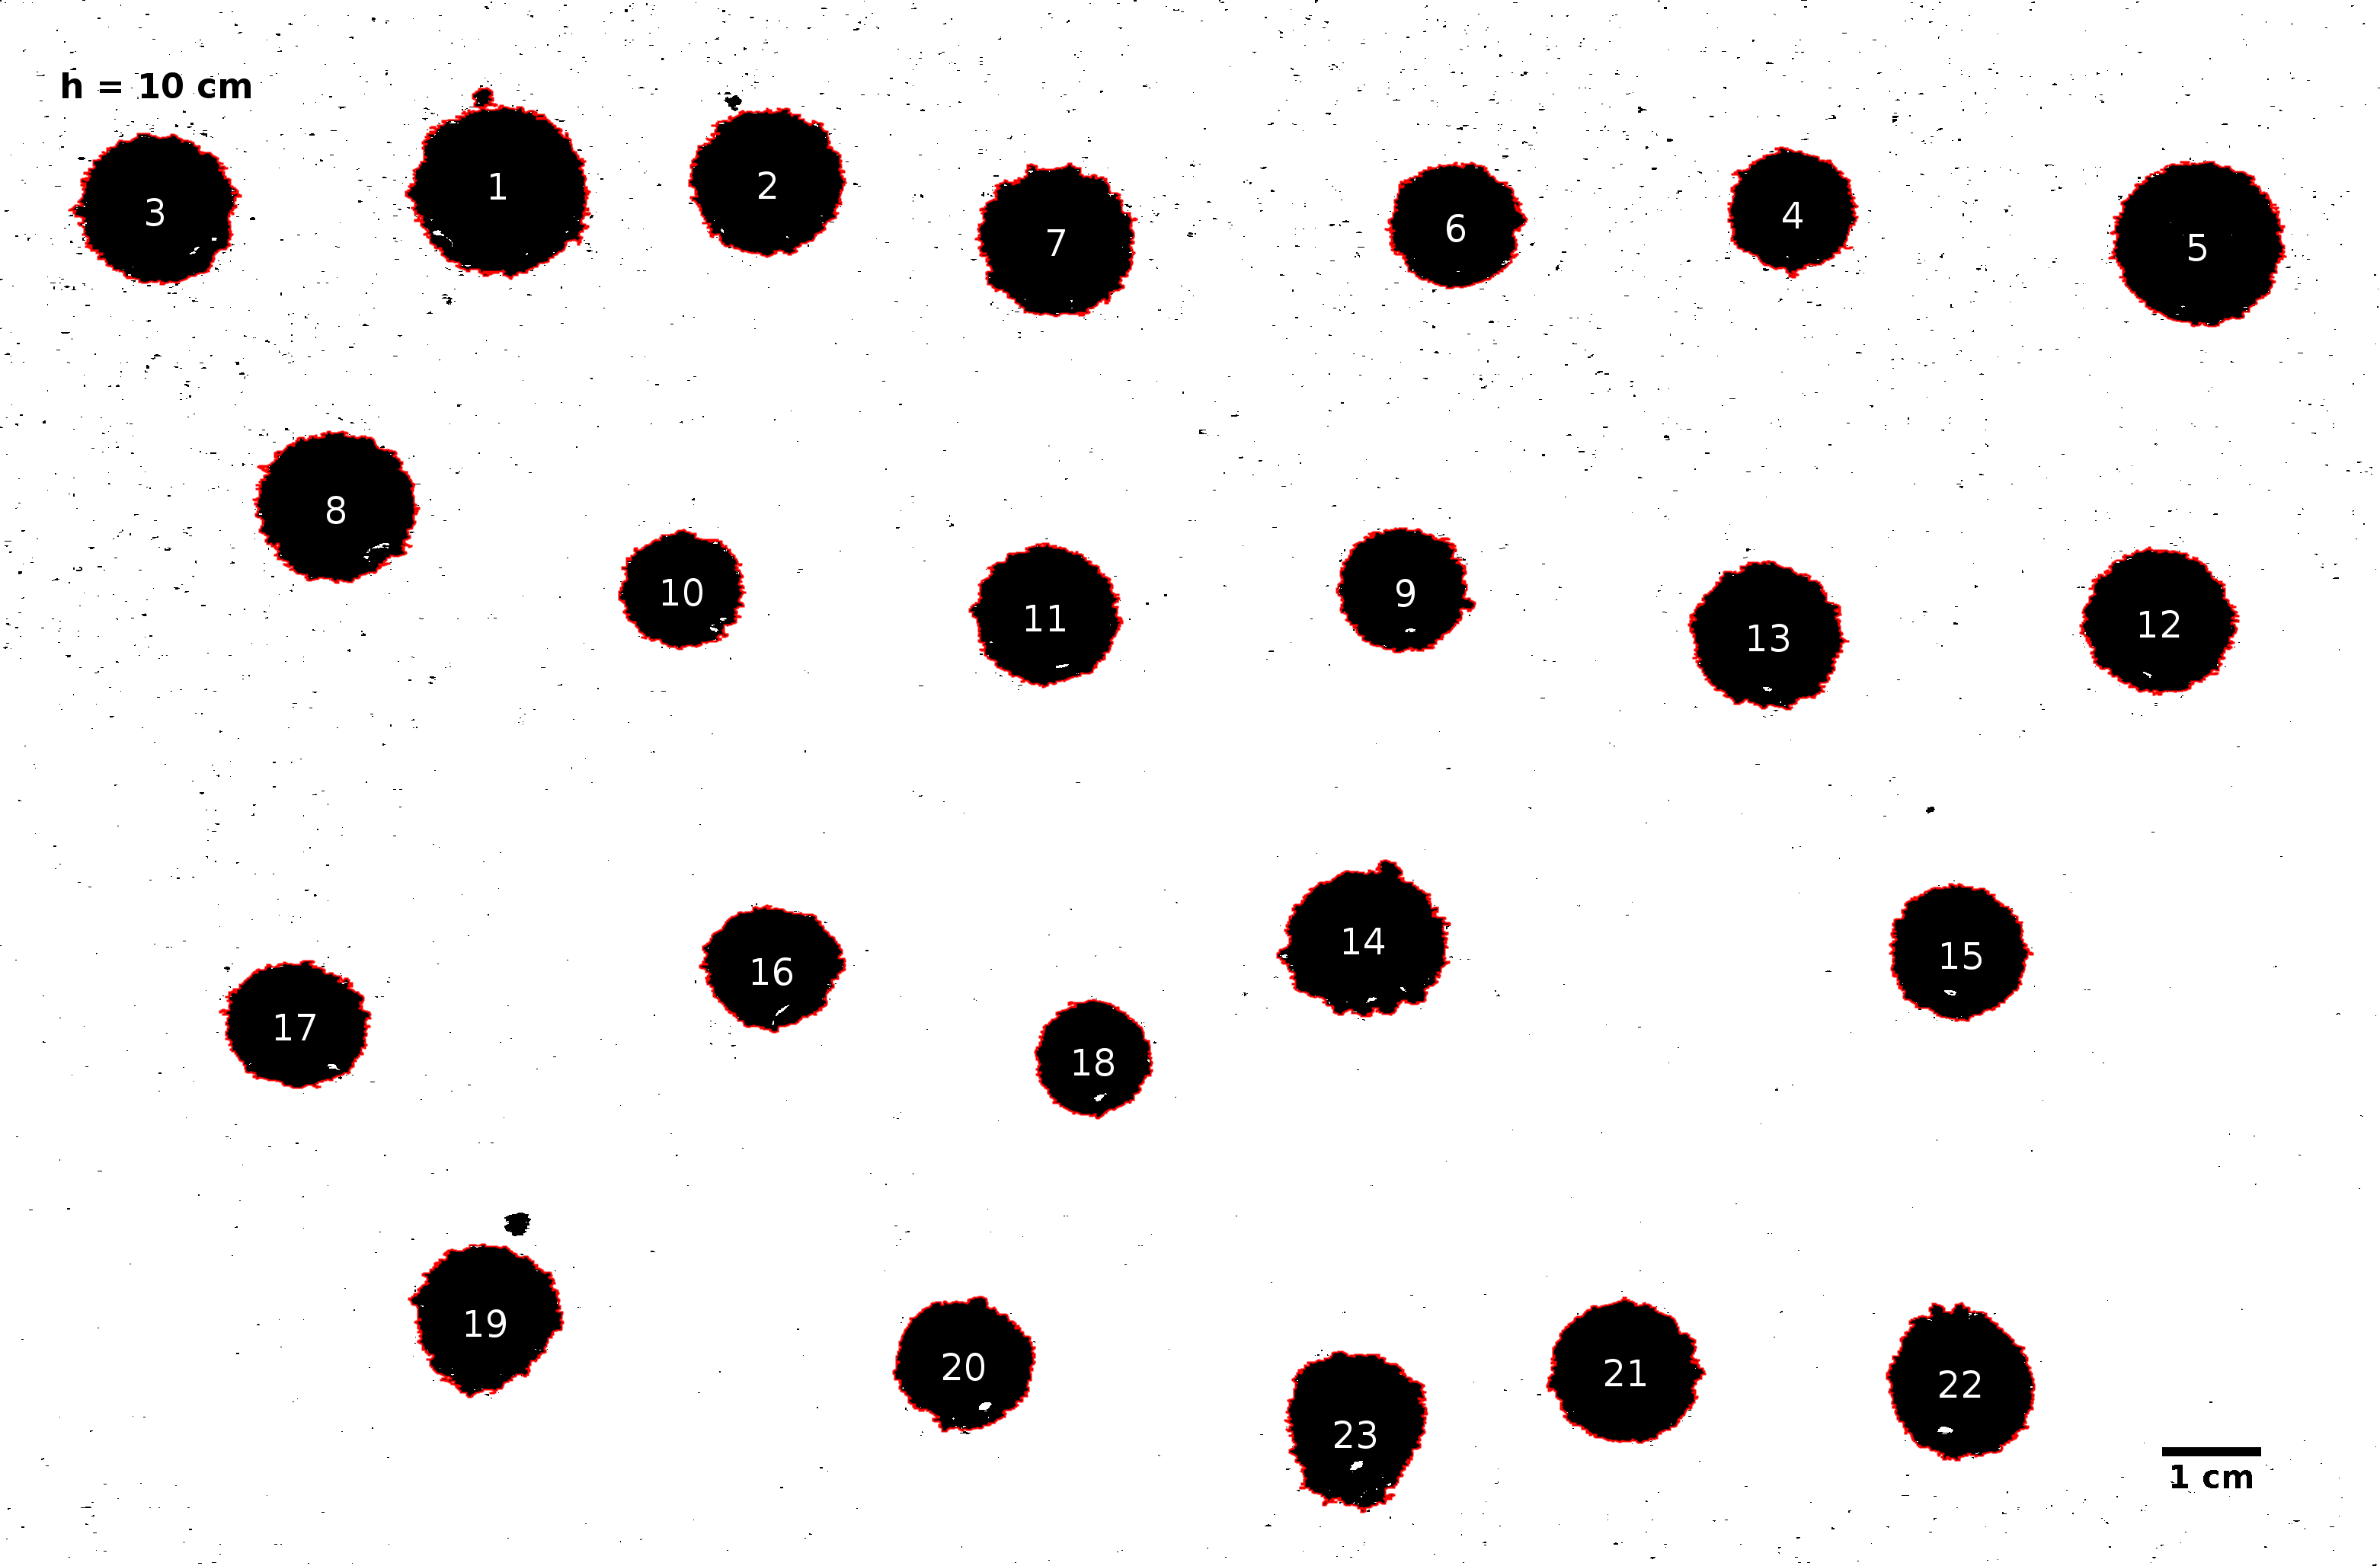
\includegraphics[width=0.66\linewidth]{src/10-1.png} \caption{Mancha de gotas
desde $10\ cm$} \label{fig:10cm-1} \end{figure}

\begin{table}[H] \centering \caption{Datos obtenidos a partir de la figura
    ~\ref{fig:20cm-1} ($h = 20\ cm)$} \label{tab:20cm} \begin{tabular}{cccccc}
        \toprule Gota & Área ($cm^2$) & Perímetro ($cm$) & Eje mayor ($cm$) &
        Eje menor ($cm$) & Dirección ($^o$) \\ \midrule 1     & 1.98 & 6.75  &
        1.64 & 1.54 & 144.94 \\ 2     & 2.08 & 7.27  & 1.66 & 1.59 & 166.41 \\
        3     & 2.36 & 7.38  & 1.76 & 1.71 & 163.07 \\ 4     & 1.79 & 6.33  &
        1.54 & 1.48 & 167.03 \\ 5     & 2.53 & 7.39  & 1.90 & 1.70 & 153.35 \\
        6     & 2.11 & 7.68  & 1.67 & 1.61 & 8.22   \\ 7     & 2.34 & 7.35  &
        1.76 & 1.69 & 161.77 \\ 8     & 2.03 & 6.89  & 1.63 & 1.59 & 12.75  \\
        9     & 2.62 & 8.22  & 1.87 & 1.78 & 4.18   \\ 10    & 2.47 & 7.83  &
        1.81 & 1.73 & 167.47 \\ 11    & 2.80 & 8.95  & 1.92 & 1.86 & 8.13   \\
        12    & 2.30 & 7.43  & 1.75 & 1.67 & 64.28  \\ 13    & 2.18 & 6.96  &
        1.70 & 1.63 & 163.64 \\ 14    & 1.76 & 6.57  & 1.53 & 1.47 & 14.81  \\
        15    & 2.23 & 7.49  & 1.71 & 1.66 & 26.08  \\ 16    & 2.38 & 6.90  &
        1.77 & 1.71 & 10.46  \\ 17    & 2.70 & 8.61  & 1.89 & 1.82 & 141.29 \\
        18    & 3.41 & 10.30 & 2.15 & 2.02 & 159.40 \\ 19    & 2.26 & 7.47  &
        1.71 & 1.69 & 37.76  \\ 20    & 2.52 & 7.82  & 1.83 & 1.75 & 101.89 \\
        21    & 1.81 & 6.66  & 1.54 & 1.50 & 32.24  \\ \midrule Media & 2.32 &
        7.54  & 1.75 & 1.68 & 90.91  \\ \bottomrule \end{tabular} \end{table}

\begin{figure}[H] \centering
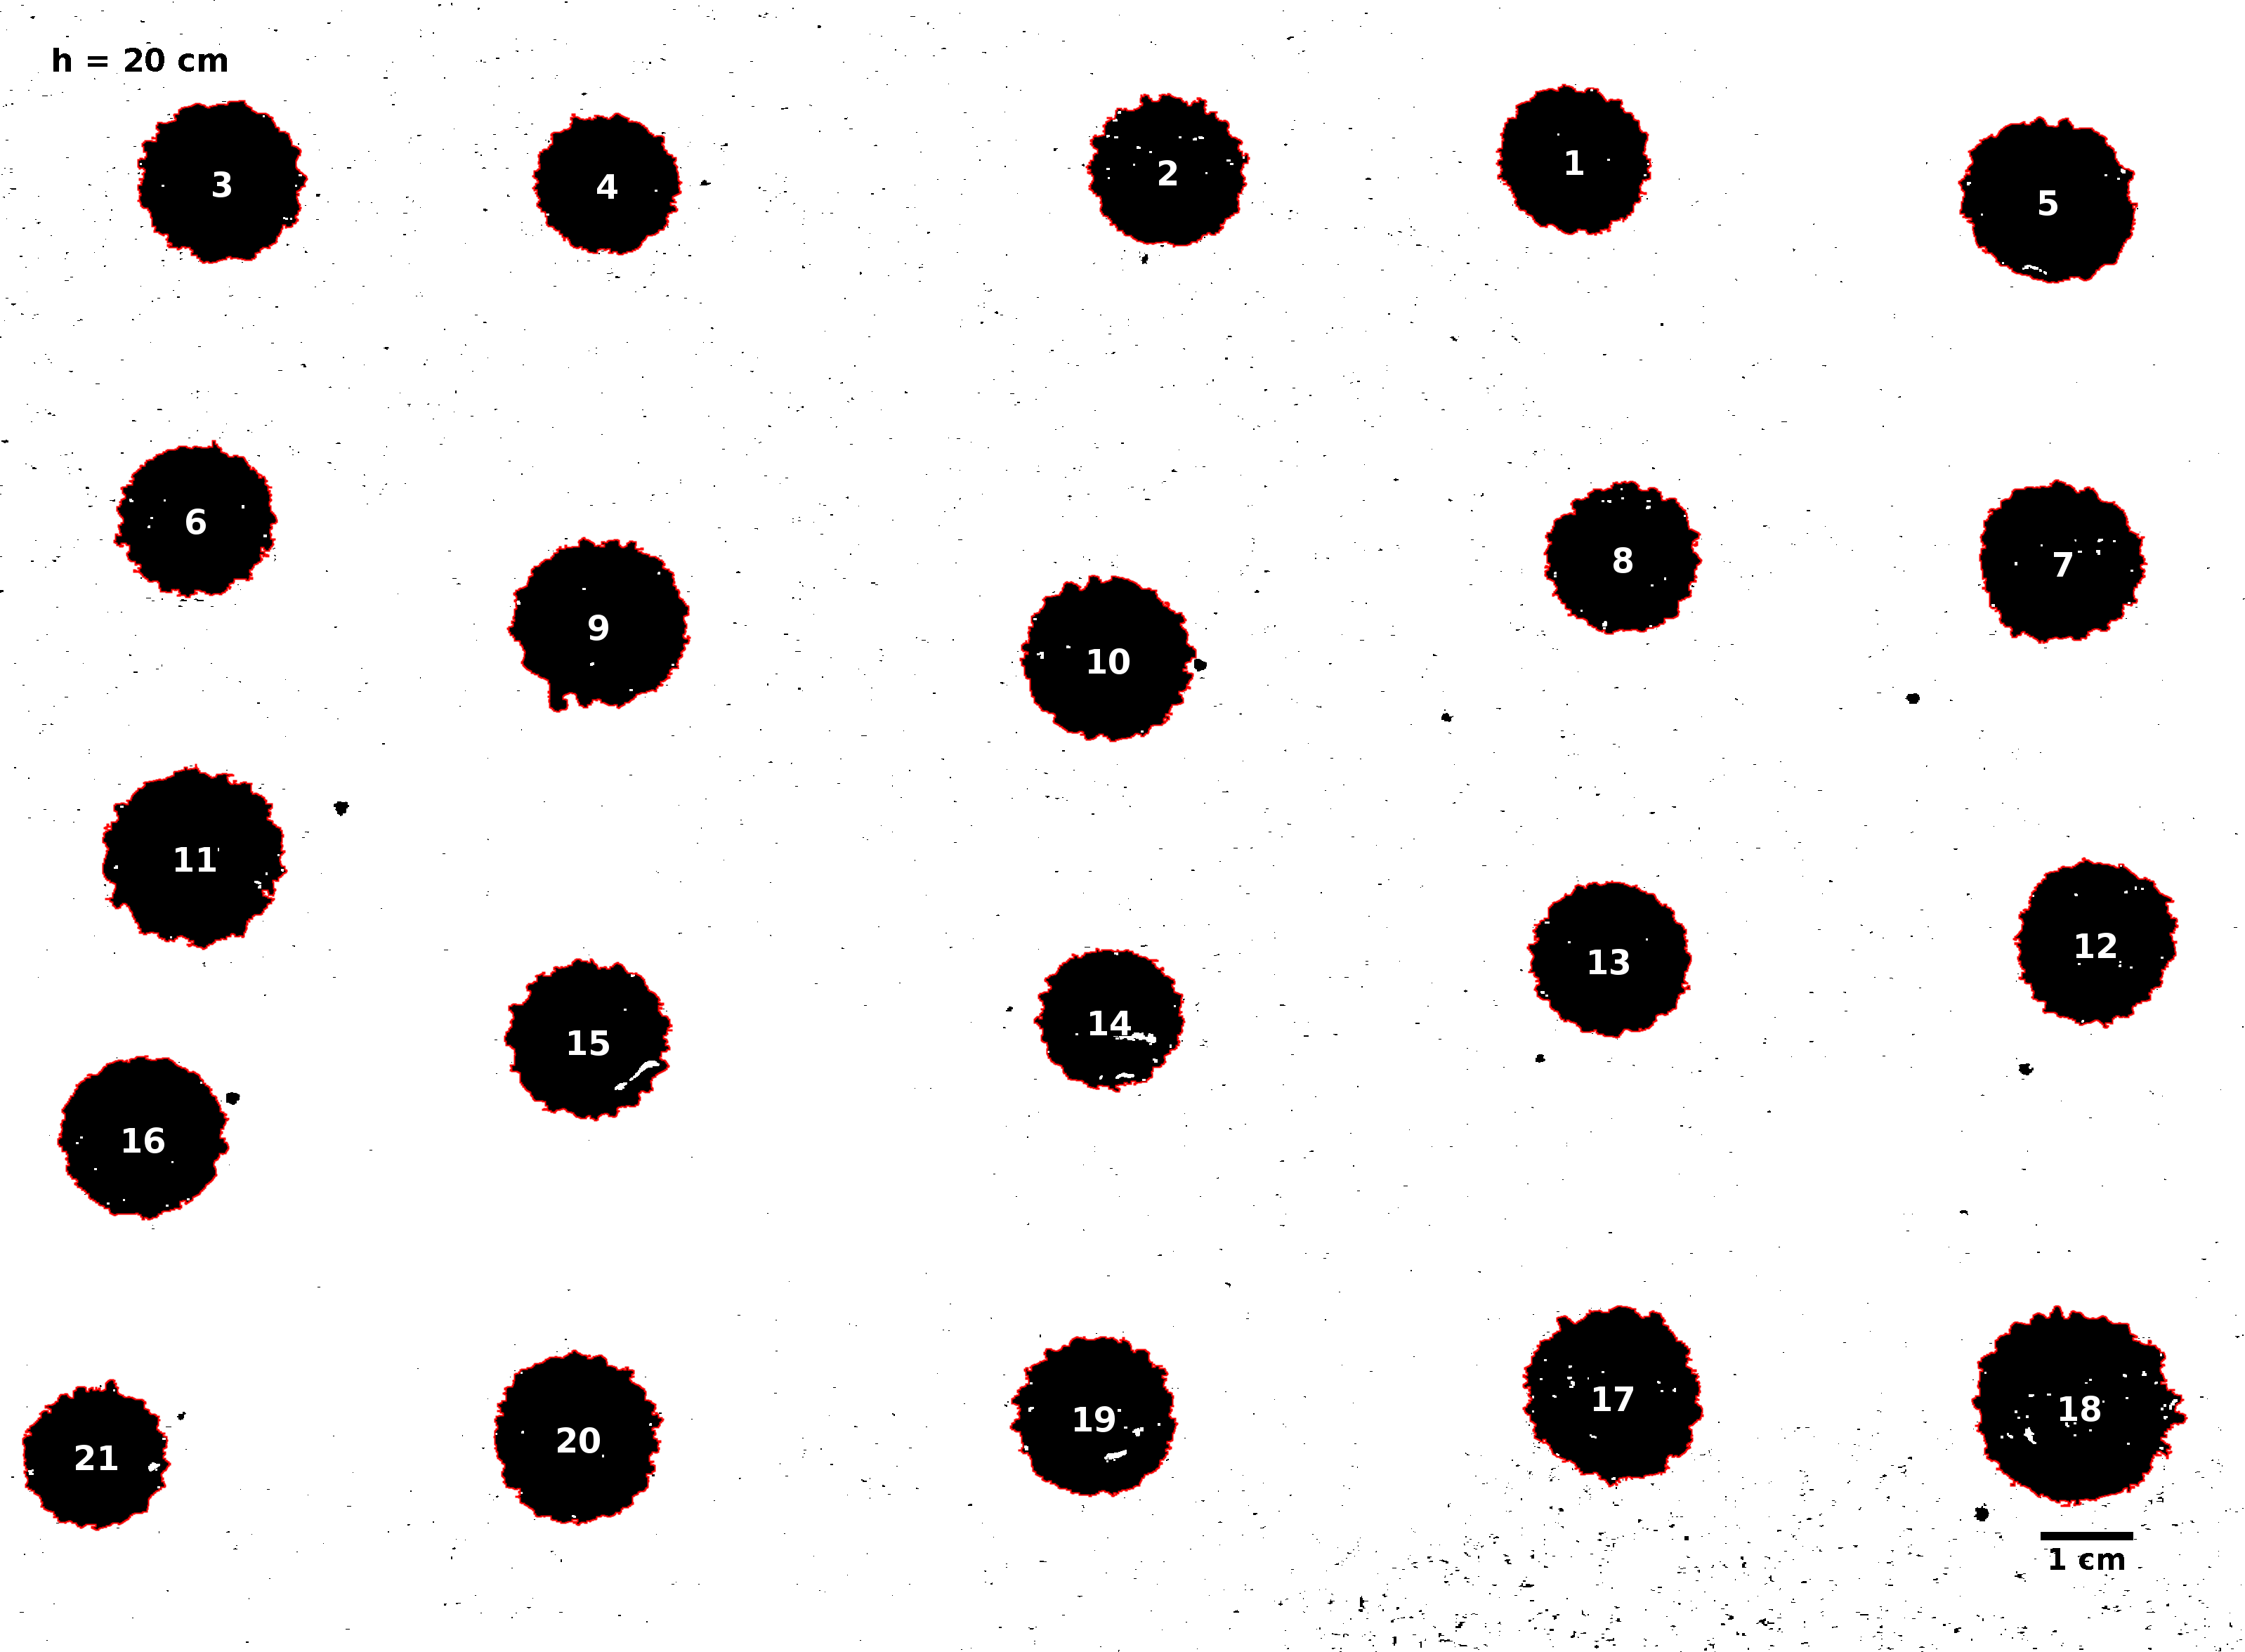
\includegraphics[width=0.75\linewidth]{src/20-1.png} \caption{Mancha de gotas
desde $20\ cm$} \label{fig:20cm-1} \end{figure}

\begin{table}[H] \centering \caption{Datos obtenidos a partir de la figura
    ~\ref{fig:30cm-1} ($h = 30\ cm$)} \label{tab:30cm} \begin{tabular}{cccccc}
        \toprule Gota & Área ($cm^2$) & Perímetro ($cm$) & Eje mayor ($cm$) &
        Eje menor ($cm$) & Dirección ($^o$) \\ \midrule 1     & 3.27 & 10.05 &
        2.11 & 1.97 & 175.54 \\ 2     & 2.58 & 7.93  & 1.86 & 1.77 & 166.21 \\
        3     & 2.99 & 8.31  & 2.01 & 1.90 & 172.92 \\ 4     & 3.26 & 9.37  &
        2.06 & 2.02 & 27.07  \\ 5     & 3.33 & 10.52 & 2.08 & 2.03 & 11.79  \\
        6     & 2.98 & 8.75  & 2.00 & 1.89 & 5.73   \\ 7     & 3.20 & 9.41  &
        2.09 & 1.95 & 174.57 \\ 8     & 2.54 & 8.41  & 1.87 & 1.73 & 170.57 \\
        9     & 2.74 & 8.75  & 1.91 & 1.83 & 98.60  \\ 10    & 3.86 & 9.81  &
        2.25 & 2.18 & 169.21 \\ 11    & 2.82 & 9.03  & 1.94 & 1.85 & 162.24 \\
        12    & 3.27 & 9.28  & 2.09 & 2.00 & 171.87 \\ 13    & 3.40 & 9.78  &
        2.11 & 2.05 & 179.65 \\ 14    & 3.05 & 8.96  & 2.00 & 1.94 & 13.51  \\
        15    & 2.72 & 8.72  & 2.02 & 1.71 & 9.71   \\ 16    & 2.08 & 6.71  &
        1.78 & 1.49 & 89.49  \\ 17    & 3.35 & 9.27  & 2.13 & 2.00 & 164.78 \\
        18    & 2.93 & 8.90  & 1.98 & 1.88 & 175.60 \\ 19    & 4.23 & 11.69 &
        2.38 & 2.26 & 58.01  \\ 20    & 3.72 & 9.34  & 2.21 & 2.14 & 24.44  \\
        21    & 2.96 & 10.02 & 2.00 & 1.88 & 151.15 \\ 22    & 3.27 & 9.12  &
        2.08 & 2.00 & 19.53  \\ 23    & 3.31 & 9.68  & 2.08 & 2.02 & 76.35  \\
    24    & 2.74 & 8.32  & 1.92 & 1.81 & 11.35  \\ \midrule Media & 3.11 & 9.17
          & 2.04 & 1.93 & 103.33 \\ \bottomrule \end{tabular} \end{table}

\begin{figure}[H] \centering
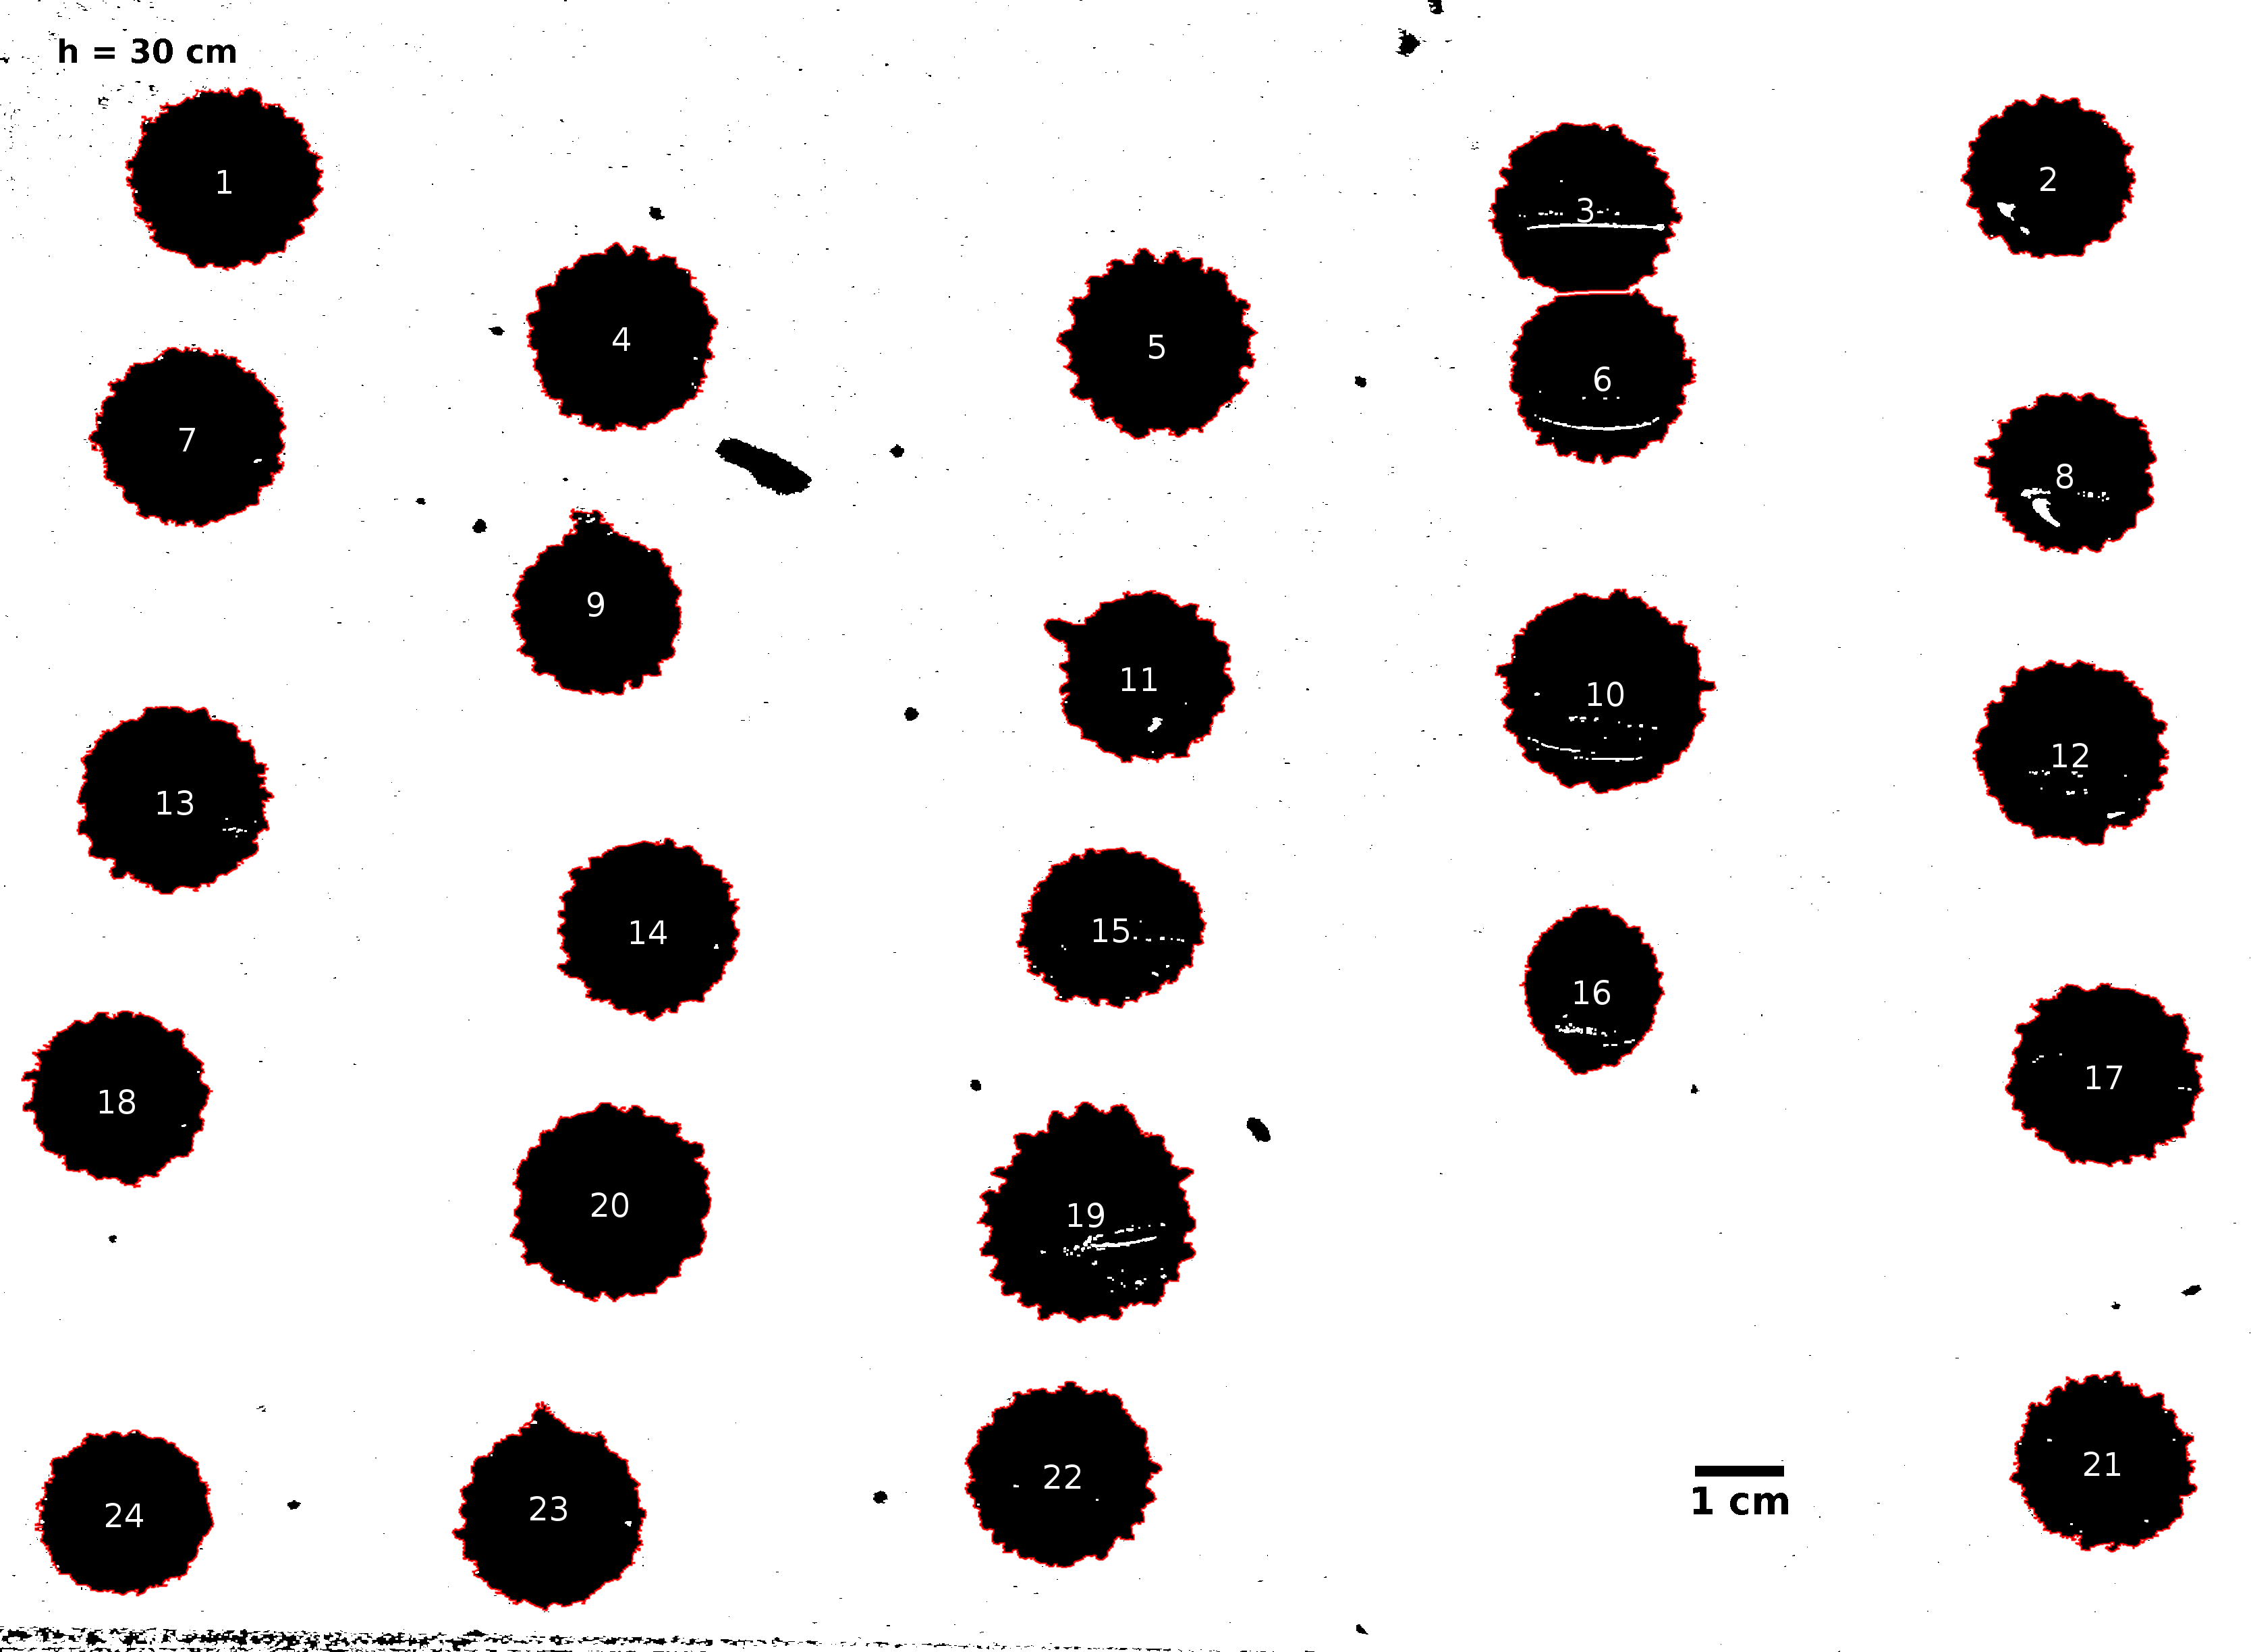
\includegraphics[width=0.66\linewidth]{src/30-1.png} \caption{Mancha de gotas
desde $30\ cm$} \label{fig:30cm-1} \end{figure}

\begin{table}[H] \centering \caption{Datos obtenidos a partir de la figura
    ~\ref{fig:40cm-1} ($h=40\ cm)$} \label{tab:40cm} \begin{tabular}{cccccc}
        \toprule Gota & Área ($cm^2$) & Perímetro ($cm$) & Eje mayor ($cm$) &
        Eje menor ($cm$) & Dirección ($^o$) \\ \midrule 1  & 3.16 & 12.29 &
        2.06 & 1.95 & 167.56 \\ 2  & 2.96 & 10.97 & 1.98 & 1.90 & 173.57 \\ 3
             & 3.36 & 10.36 & 2.13 & 2.01 & 167.17 \\ 4  & 3.44 & 12.16 & 2.12
             & 2.07 & 161.16 \\ 5  & 3.59 & 12.39 & 2.18 & 2.09 & 163.28 \\ 6
             & 3.46 & 11.21 & 2.12 & 2.07 & 159.61 \\ 7  & 3.35 & 12.09 & 2.12
             & 2.02 & 2.75   \\ 8  & 2.96 & 9.83  & 1.99 & 1.89 & 178.98 \\ 9
             & 3.07 & 12.17 & 2.03 & 1.92 & 177.01 \\ 10 & 3.59 & 14.33 & 2.18
             & 2.10 & 150.30 \\ 11 & 3.04 & 11.05 & 2.01 & 1.93 & 168.92 \\ 12
             & 4.02 & 14.03 & 2.33 & 2.19 & 0.66   \\ 13 & 3.33 & 13.15 & 2.07
             & 2.05 & 164.48 \\ 14 & 3.37 & 13.73 & 2.09 & 2.06 & 153.97 \\ 15
             & 3.79 & 12.61 & 2.24 & 2.15 & 149.19 \\ 16 & 2.87 & 9.38  & 1.95
             & 1.87 & 18.31  \\ 17 & 2.96 & 10.08 & 1.98 & 1.90 & 159.61 \\ 18
             & 3.98 & 11.89 & 2.30 & 2.20 & 1.50   \\ 19 & 3.49 & 13.40 & 2.13
             & 2.08 & 164.65 \\ 20 & 4.64 & 16.91 & 2.47 & 2.40 & 150.18 \\ 21
             & 2.97 & 9.99  & 1.99 & 1.90 & 24.94  \\ 22 & 3.68 & 13.25 & 2.20
             & 2.13 & 143.60 \\ 23 & 3.51 & 13.04 & 2.14 & 2.09 & 9.73   \\ 24
             & 3.05 & 11.47 & 2.02 & 1.92 & 17.54  \\ 25 & 3.06 & 11.93 & 1.99
             & 1.95 & 171.50 \\ 26 & 2.93 & 11.05 & 1.95 & 1.91 & 142.70 \\
        \midrule Media  & 3.37 & 12.11 & 2.11 & 2.03 & 120.88 \\ \bottomrule
    \end{tabular} \end{table}

\begin{figure}[H] \centering
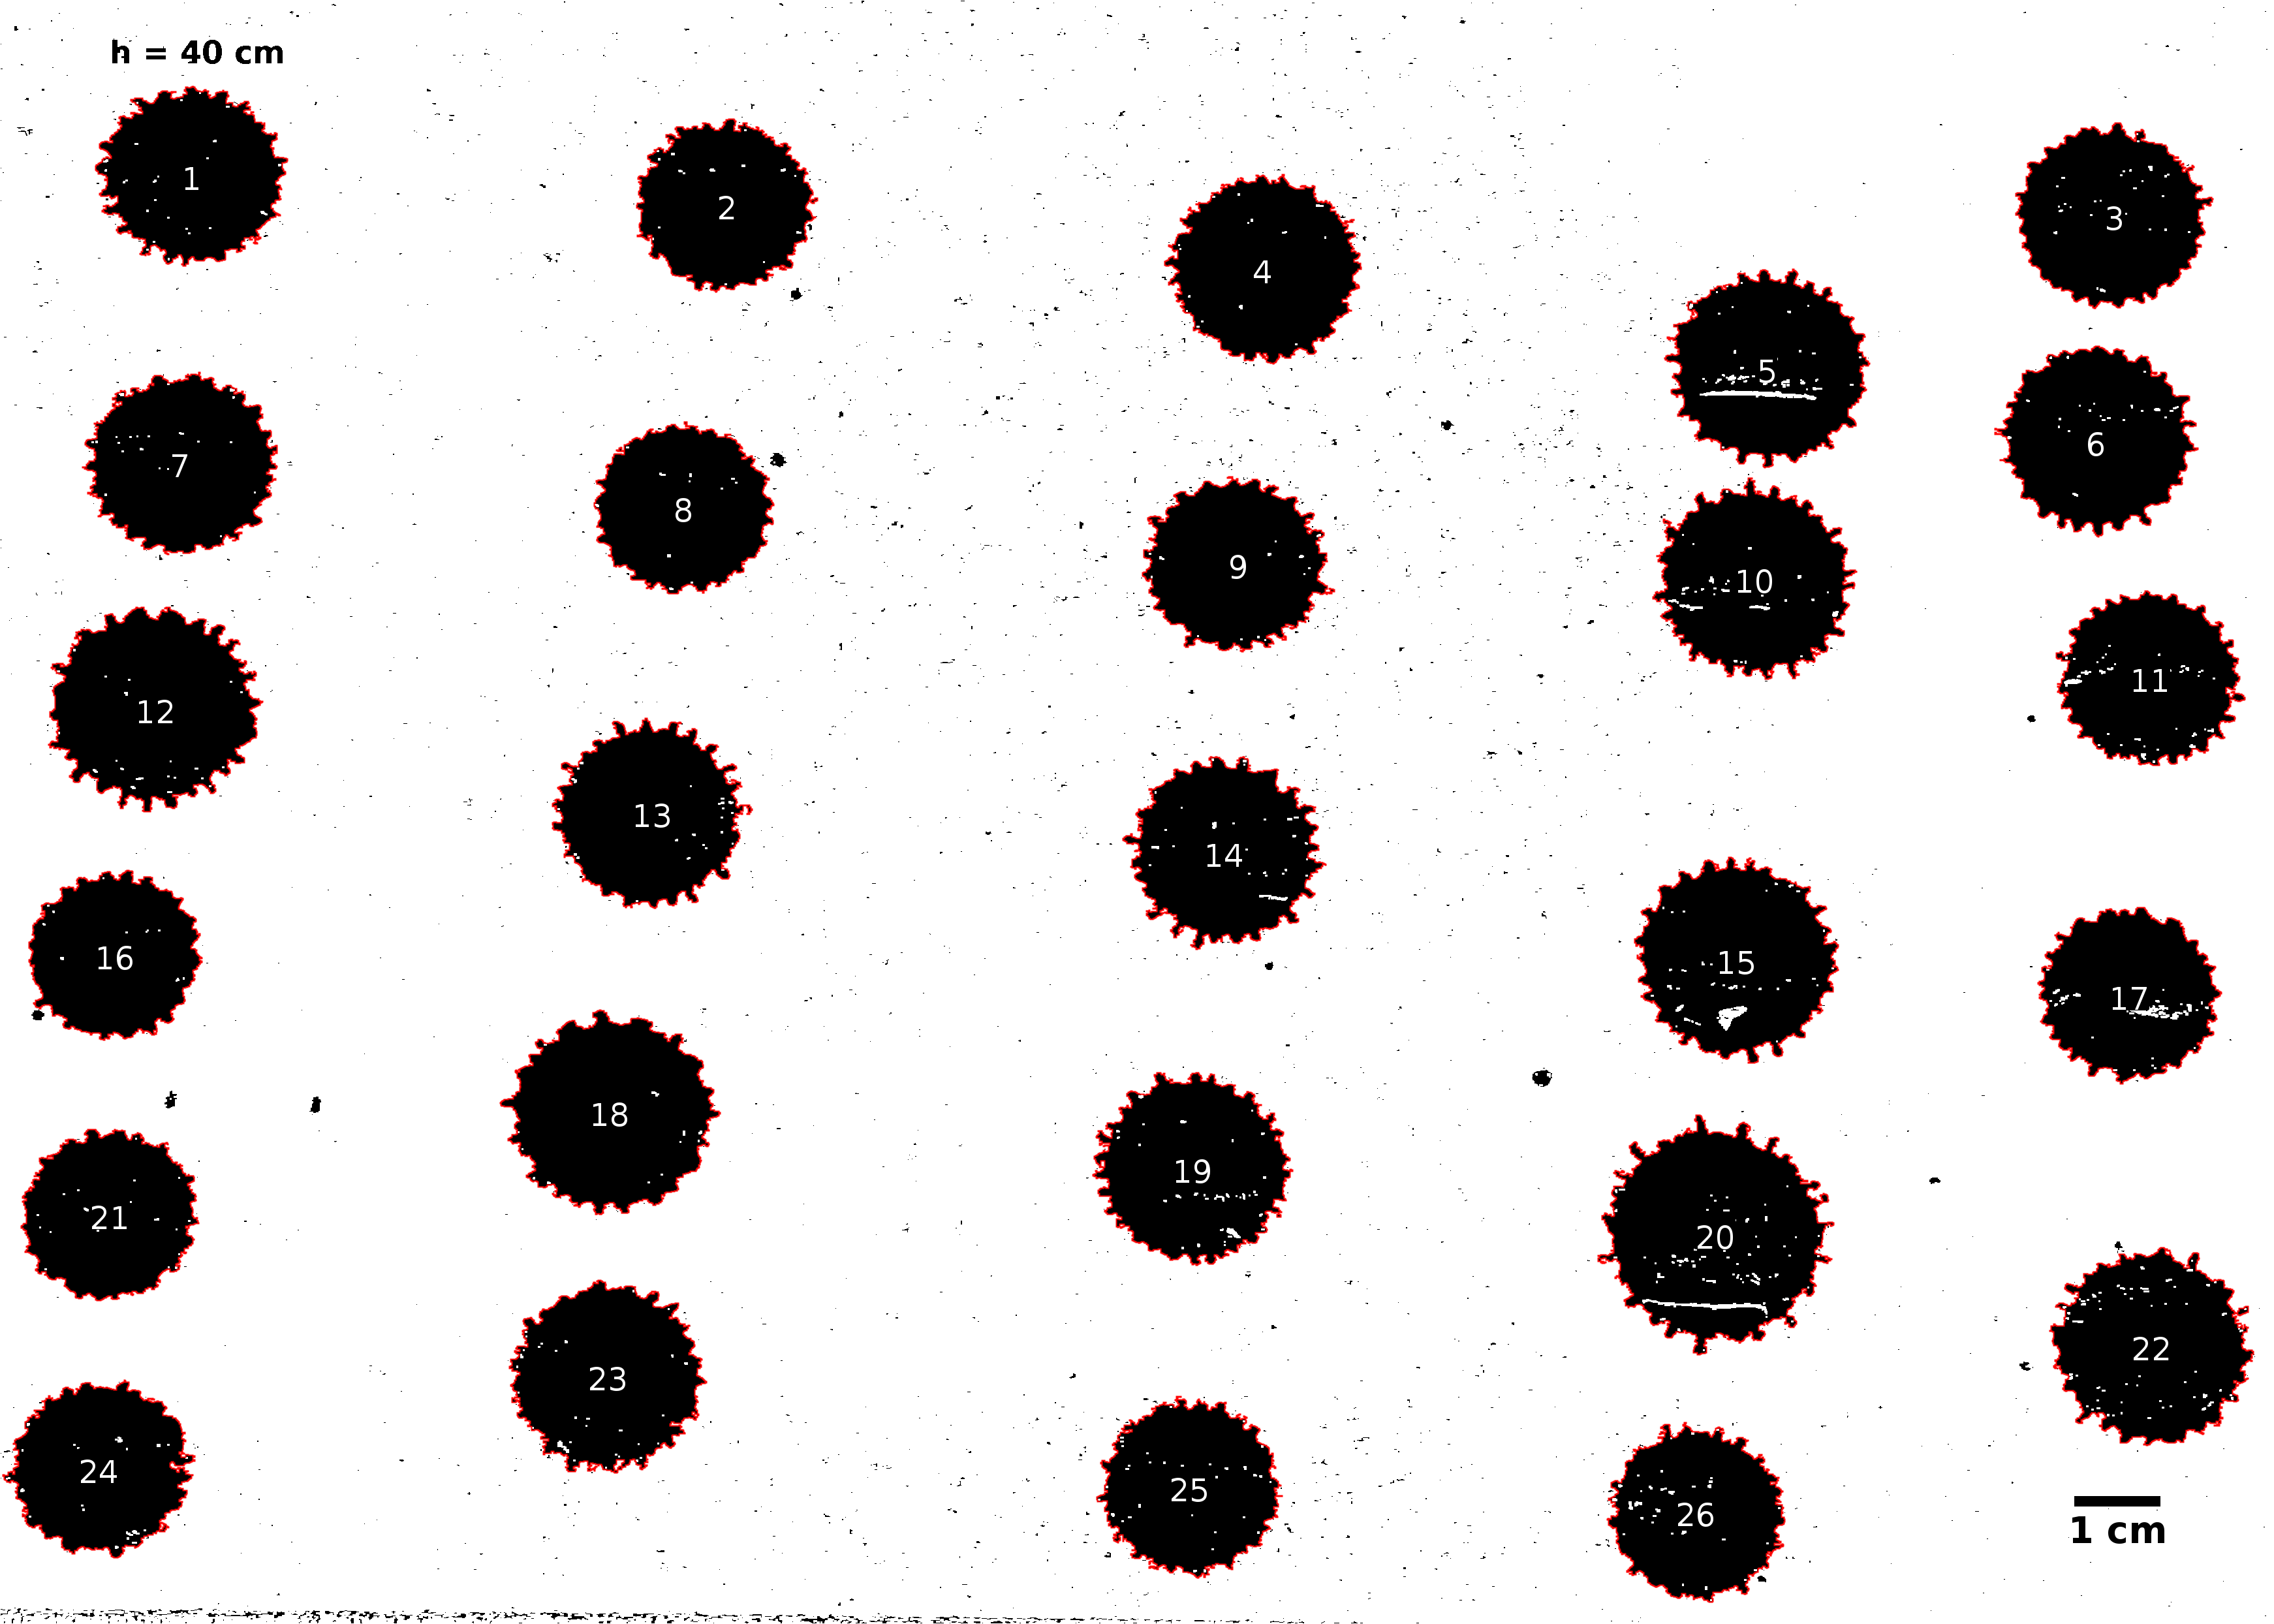
\includegraphics[width=0.60\linewidth]{src/40-1.png} \caption{Mancha de gotas
desde $40\ cm$} \label{fig:40cm-1} \end{figure}

\begin{table}[H] \centering \caption{Datos obtenidos a partir de la figura
    ~\ref{fig:50cm-1} ($h=50\ cm)$} \label{tab:50cm} \begin{tabular}{cccccc}
        \toprule Gota & Área ($cm^2$) & Perímetro ($cm$) & Eje mayor ($cm$) &
        Eje menor ($cm$) & Dirección ($^o$) \\ \midrule 1  & 3.34 & 11.57 &
        2.12 & 2.01 & 170.41 \\ 2  & 3.32 & 11.98 & 2.12 & 2.00 & 171.67 \\ 3
             & 3.79 & 11.97 & 2.25 & 2.14 & 143.64 \\ 4  & 3.77 & 13.31 & 2.37
             & 2.03 & 102.56 \\ 5  & 2.90 & 9.64  & 1.97 & 1.87 & 178.39 \\ 6
             & 3.29 & 11.47 & 2.07 & 2.02 & 147.46 \\ 7  & 3.48 & 11.31 & 2.25
             & 1.97 & 13.11  \\ 8  & 3.59 & 11.14 & 2.21 & 2.07 & 175.96 \\ 9
             & 2.79 & 9.74  & 1.91 & 1.85 & 177.78 \\ 10 & 3.00 & 9.64  & 2.04
             & 1.87 & 119.35 \\ 11 & 3.46 & 10.89 & 2.17 & 2.03 & 170.56 \\ 12
             & 3.83 & 12.90 & 2.27 & 2.14 & 144.28 \\ 13 & 3.60 & 11.69 & 2.23
             & 2.05 & 10.36  \\ 14 & 3.58 & 10.68 & 2.18 & 2.10 & 170.99 \\ 15
             & 3.71 & 11.79 & 2.26 & 2.08 & 20.50  \\ 16 & 4.30 & 13.60 & 2.48
             & 2.21 & 174.36 \\ 17 & 3.08 & 10.45 & 2.04 & 1.93 & 164.98 \\ 18
             & 3.85 & 12.53 & 2.36 & 2.08 & 131.89 \\ 19 & 3.27 & 10.97 & 2.05
             & 2.03 & 71.67  \\ 20 & 3.76 & 13.54 & 2.20 & 2.18 & 152.77 \\ 21
             & 3.73 & 14.05 & 2.21 & 2.15 & 106.25 \\ 22 & 2.88 & 9.60  & 1.94
             & 1.89 & 28.77  \\ 23 & 3.12 & 11.12 & 2.07 & 1.92 & 127.66 \\
    \midrule Media & 3.45 & 11.55 & 2.16 & 2.03 & 125.02 \\ \bottomrule
\end{tabular} \end{table}

\begin{figure}[H] \centering
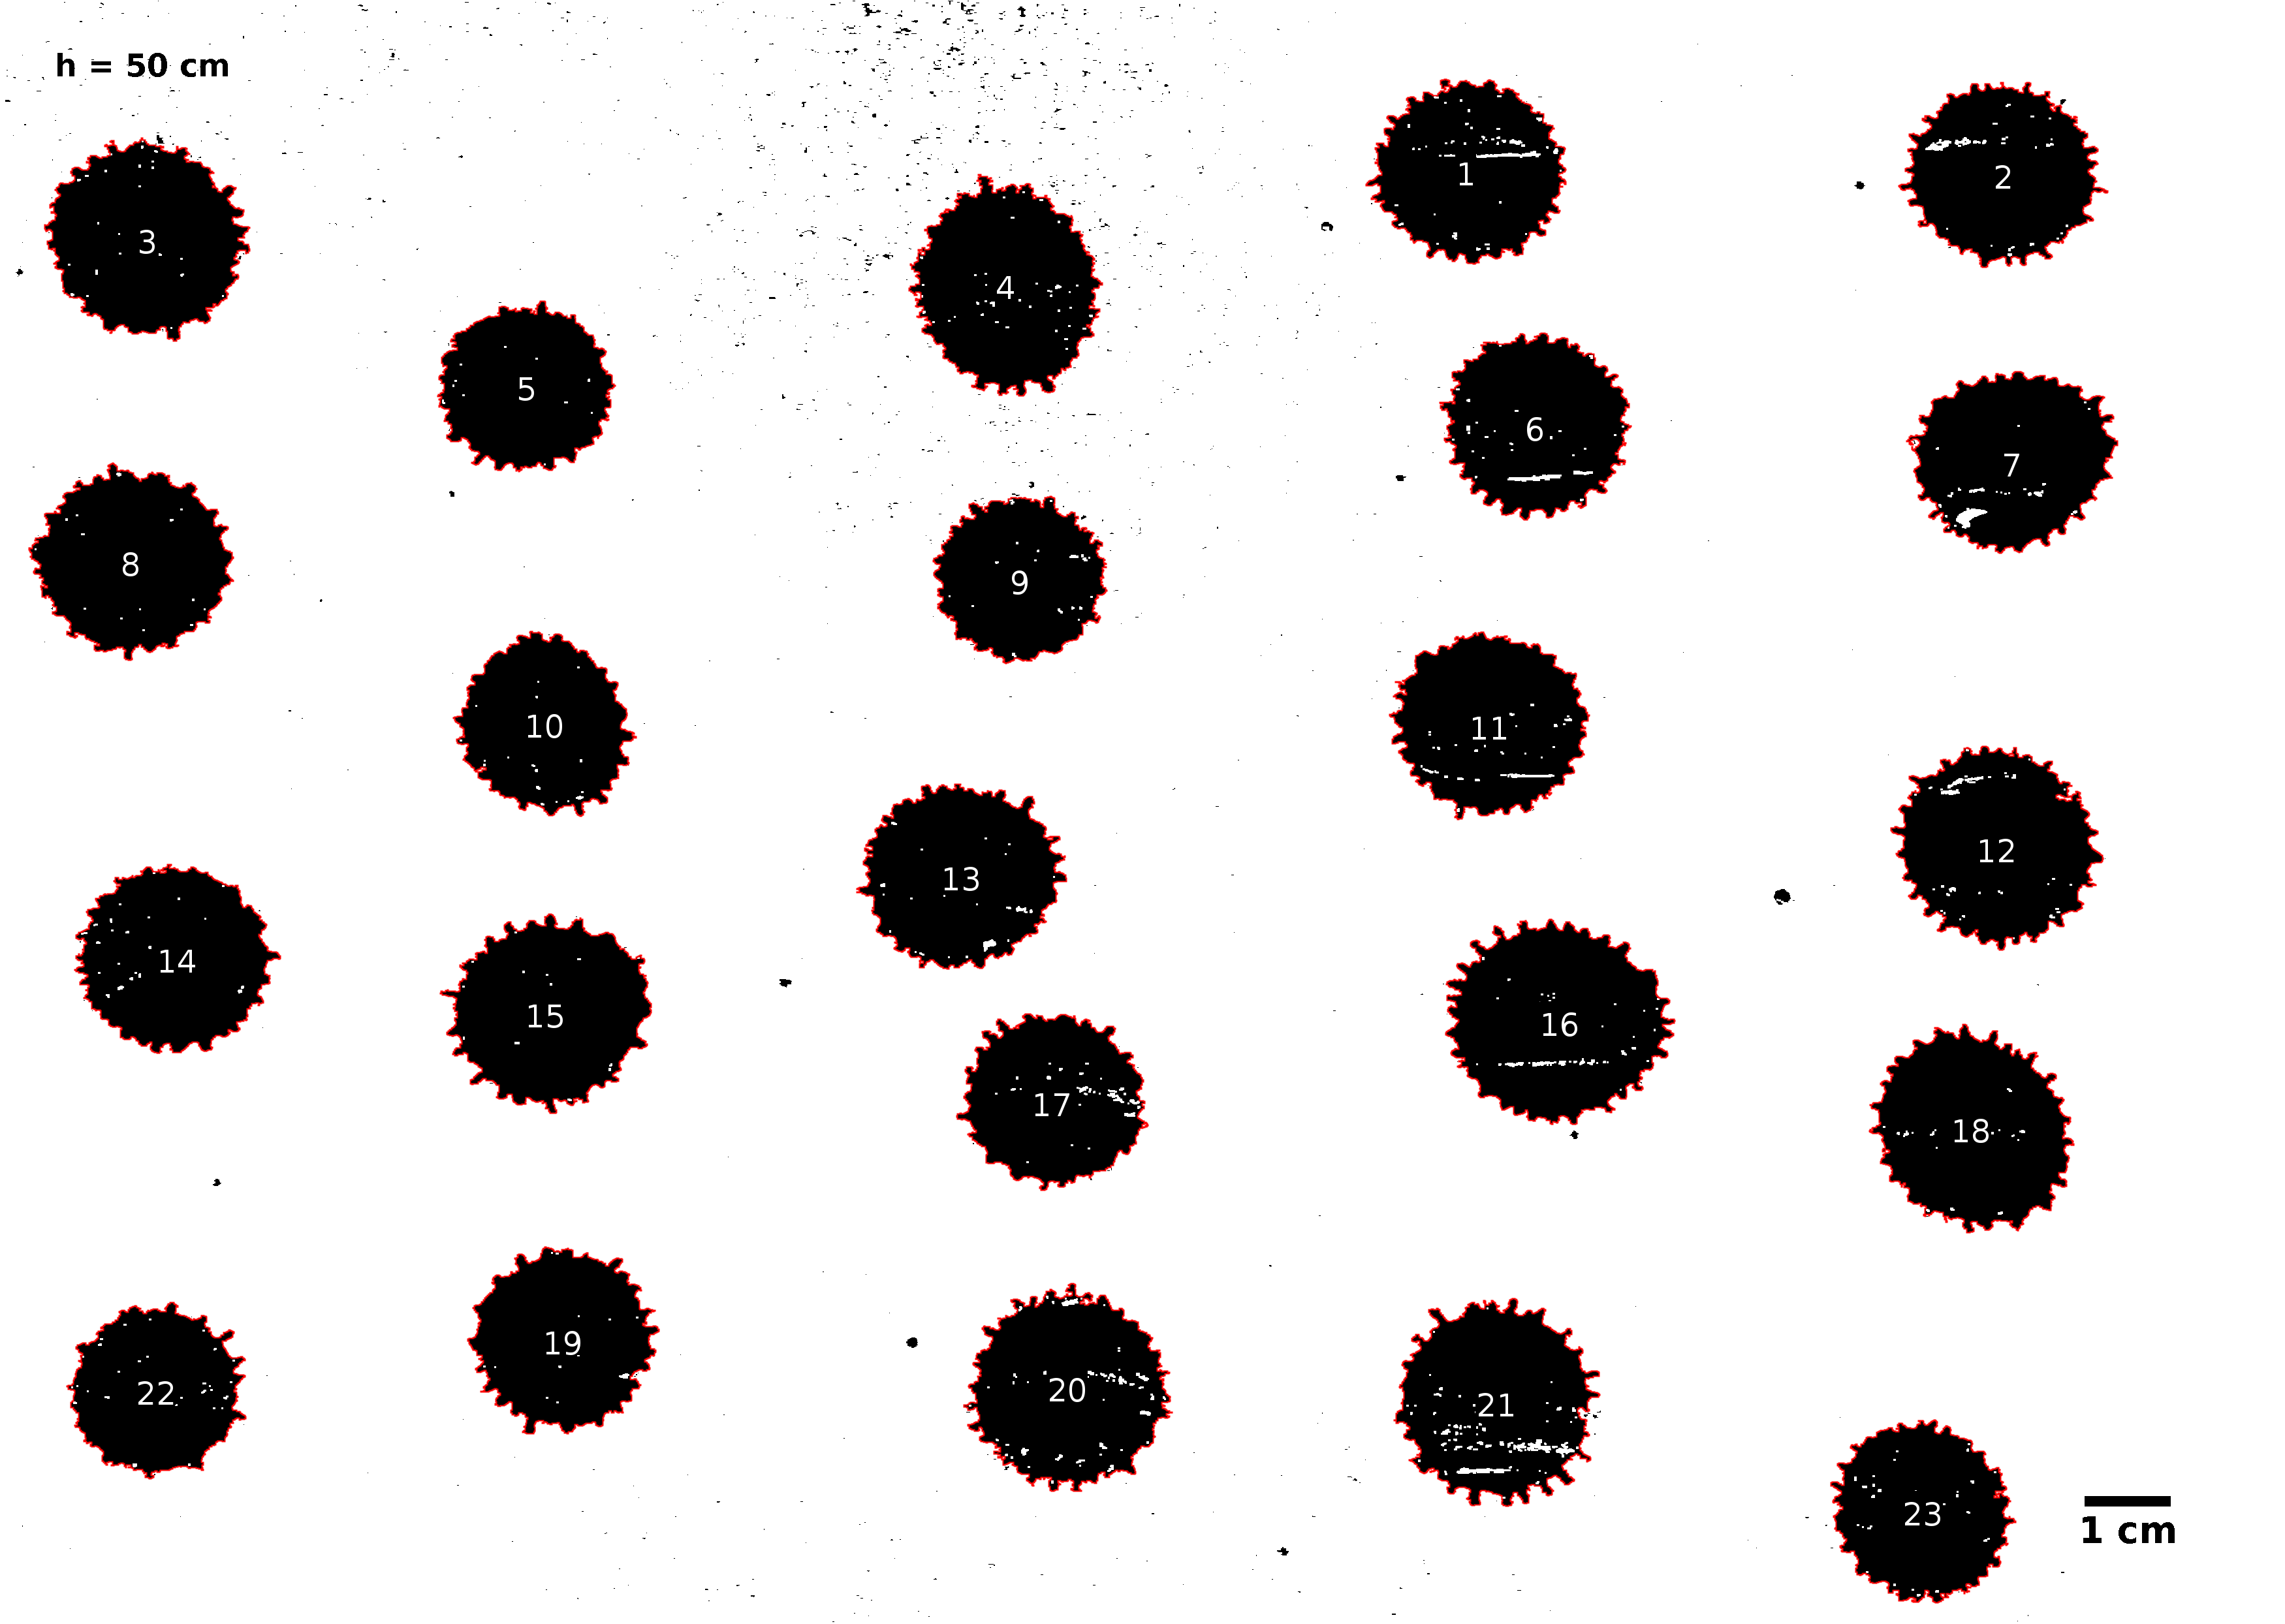
\includegraphics[width=0.75\linewidth]{src/50-1.png} \caption{Mancha de gotas
desde $50\ cm$} \label{fig:50cm-1} \end{figure}

\begin{table}[H] \centering \caption{Datos obtenidos a partir de la figura
    ~\ref{fig:60cm-1} ($h=60\ cm)$} \label{tab:60cm} \begin{tabular}{cccccc}
        \toprule Gota & Área ($cm^2$) & Perímetro ($cm$) & Eje mayor ($cm$) &
        Eje menor ($cm$) & Dirección ($^o$) \\ \midrule 1  & 3.37 & 11.37 &
        2.16 & 1.99 & 2.68   \\ 2  & 3.89 & 12.97 & 2.27 & 2.18 & 21.26  \\ 3
             & 4.23 & 13.13 & 2.40 & 2.25 & 56.06  \\ 4  & 3.54 & 13.41 & 2.16
             & 2.09 & 156.31 \\ 5  & 3.86 & 12.72 & 2.26 & 2.17 & 165.98 \\ 6
             & 3.80 & 11.05 & 2.23 & 2.17 & 164.23 \\ 7  & 3.69 & 12.28 & 2.26
             & 2.08 & 2.06   \\ 8  & 3.68 & 13.78 & 2.19 & 2.14 & 163.63 \\ 9
             & 3.61 & 12.53 & 2.21 & 2.08 & 164.50 \\ 10 & 4.01 & 12.27 & 2.41
             & 2.12 & 161.83 \\ 11 & 3.47 & 12.28 & 2.14 & 2.07 & 169.32 \\ 12
             & 3.50 & 10.62 & 2.21 & 2.02 & 179.48 \\ 13 & 2.50 & 11.44 & 1.80
             & 1.77 & 44.35  \\ 14 & 4.04 & 13.55 & 2.32 & 2.22 & 10.63  \\ 15
             & 3.44 & 10.83 & 2.15 & 2.04 & 177.14 \\ 16 & 3.36 & 9.98  & 2.12
             & 2.02 & 178.34 \\ 17 & 3.96 & 12.07 & 2.26 & 2.23 & 122.76 \\ 18
             & 3.53 & 11.79 & 2.12 & 2.12 & 90.69  \\ 19 & 4.46 & 14.42 & 2.44
             & 2.33 & 161.77 \\ 20 & 3.81 & 12.46 & 2.26 & 2.15 & 143.93 \\ 21
             & 3.60 & 10.06 & 2.17 & 2.12 & 6.98   \\ 22 & 3.51 & 12.12 & 2.14
             & 2.09 & 2.24   \\ 23 & 4.39 & 13.95 & 2.46 & 2.27 & 164.27 \\ 24
             & 3.80 & 11.90 & 2.21 & 2.19 & 82.64  \\ 25 & 4.33 & 13.76 & 2.42
             & 2.28 & 11.67  \\ 26 & 3.36 & 11.18 & 2.19 & 1.96 & 2.88   \\ 27
             & 3.63 & 11.87 & 2.17 & 2.13 & 127.16 \\ \midrule Media & 3.72 &
    12.21 & 2.23 & 2.12 & 101.29 \\ \bottomrule \end{tabular} \end{table}

\begin{figure}[H] \centering
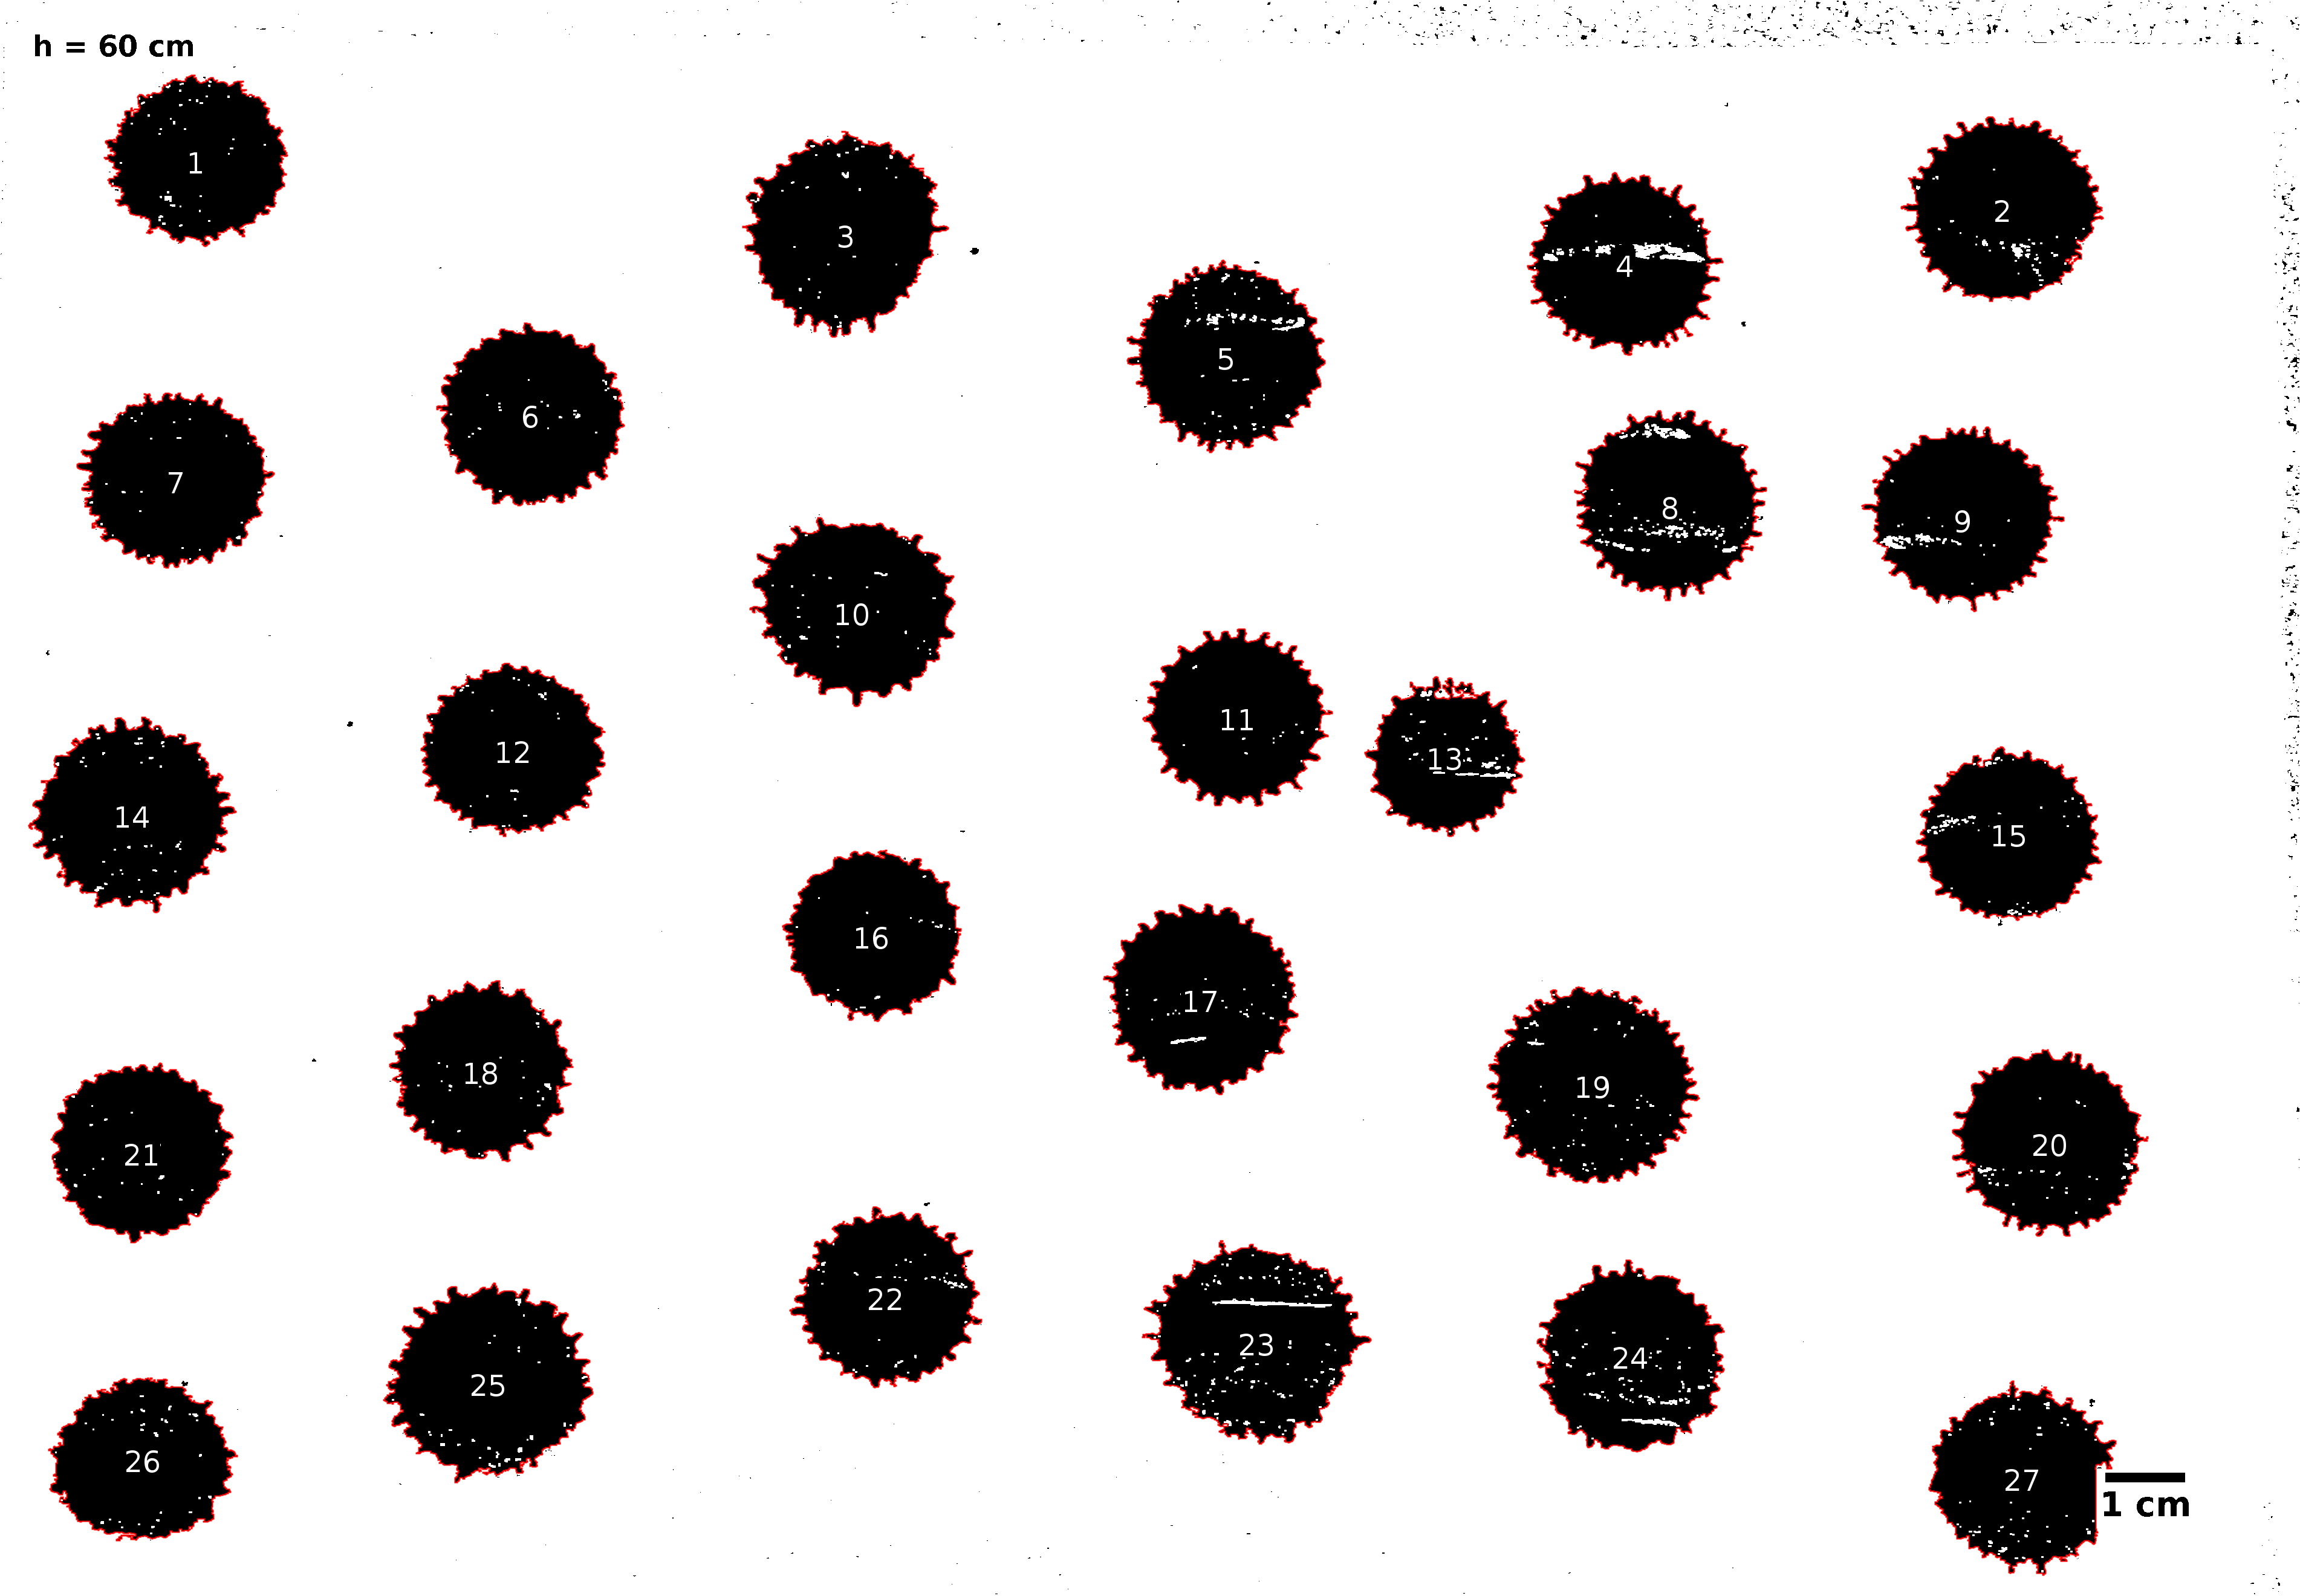
\includegraphics[width=0.60\linewidth]{src/60-1.png} \caption{Mancha de gotas
desde $60\ cm$} \label{fig:60cm-1} \end{figure}

\begin{table}[H] \centering \caption{Datos obtenidos a partir de la figura
    ~\ref{fig:70cm-1} ($h=70\ cm)$} \label{tab:70cm} \begin{tabular}{cccccc}
        \toprule Gota & Área ($cm^2$) & Perímetro ($cm$) & Eje mayor ($cm$) &
        Eje menor ($cm$) & Dirección ($^o$) \\ \midrule 1  & 3.22 & 14.25 &
        2.11 & 1.94 & 133.96 \\ 2  & 3.71 & 12.40 & 2.26 & 2.09 & 159.53 \\ 3
             & 3.57 & 12.94 & 2.15 & 2.11 & 161.77 \\ 4  & 2.60 & 11.38 & 1.87
             & 1.77 & 171.31 \\ 5  & 3.80 & 14.06 & 2.22 & 2.18 & 9.24   \\ 6
             & 3.95 & 13.24 & 2.36 & 2.14 & 38.76  \\ 7  & 2.73 & 10.83 & 1.99
             & 1.75 & 24.44  \\ 8  & 4.09 & 14.05 & 2.30 & 2.26 & 159.86 \\ 9
             & 4.37 & 14.87 & 2.40 & 2.32 & 117.81 \\ 10 & 3.89 & 14.02 & 2.26
             & 2.19 & 173.29 \\ 11 & 3.66 & 13.31 & 2.28 & 2.05 & 16.19  \\ 12
             & 3.89 & 14.33 & 2.25 & 2.20 & 171.22 \\ 13 & 3.02 & 11.07 & 2.04
             & 1.89 & 162.40 \\ 14 & 3.30 & 11.70 & 2.12 & 1.98 & 2.58   \\ 15
             & 4.10 & 16.04 & 2.33 & 2.24 & 155.05 \\ 16 & 3.30 & 12.65 & 2.11
             & 1.99 & 39.72  \\ 17 & 3.81 & 13.95 & 2.24 & 2.16 & 143.01 \\ 18
             & 4.60 & 15.47 & 2.47 & 2.37 & 156.60 \\ 19 & 4.80 & 18.29 & 2.62
             & 2.33 & 160.59 \\ 20 & 3.93 & 11.14 & 2.31 & 2.16 & 13.97  \\ 21
             & 4.51 & 15.04 & 2.46 & 2.34 & 169.10 \\ 22 & 4.40 & 14.45 & 2.46
             & 2.28 & 131.09 \\ 23 & 3.05 & 13.08 & 2.19 & 1.77 & 126.06 \\
    \midrule Media & 3.75 & 13.59 & 2.25 & 2.11 & 112.94 \\ \bottomrule
\end{tabular} \end{table}

\begin{figure}[H] \centering
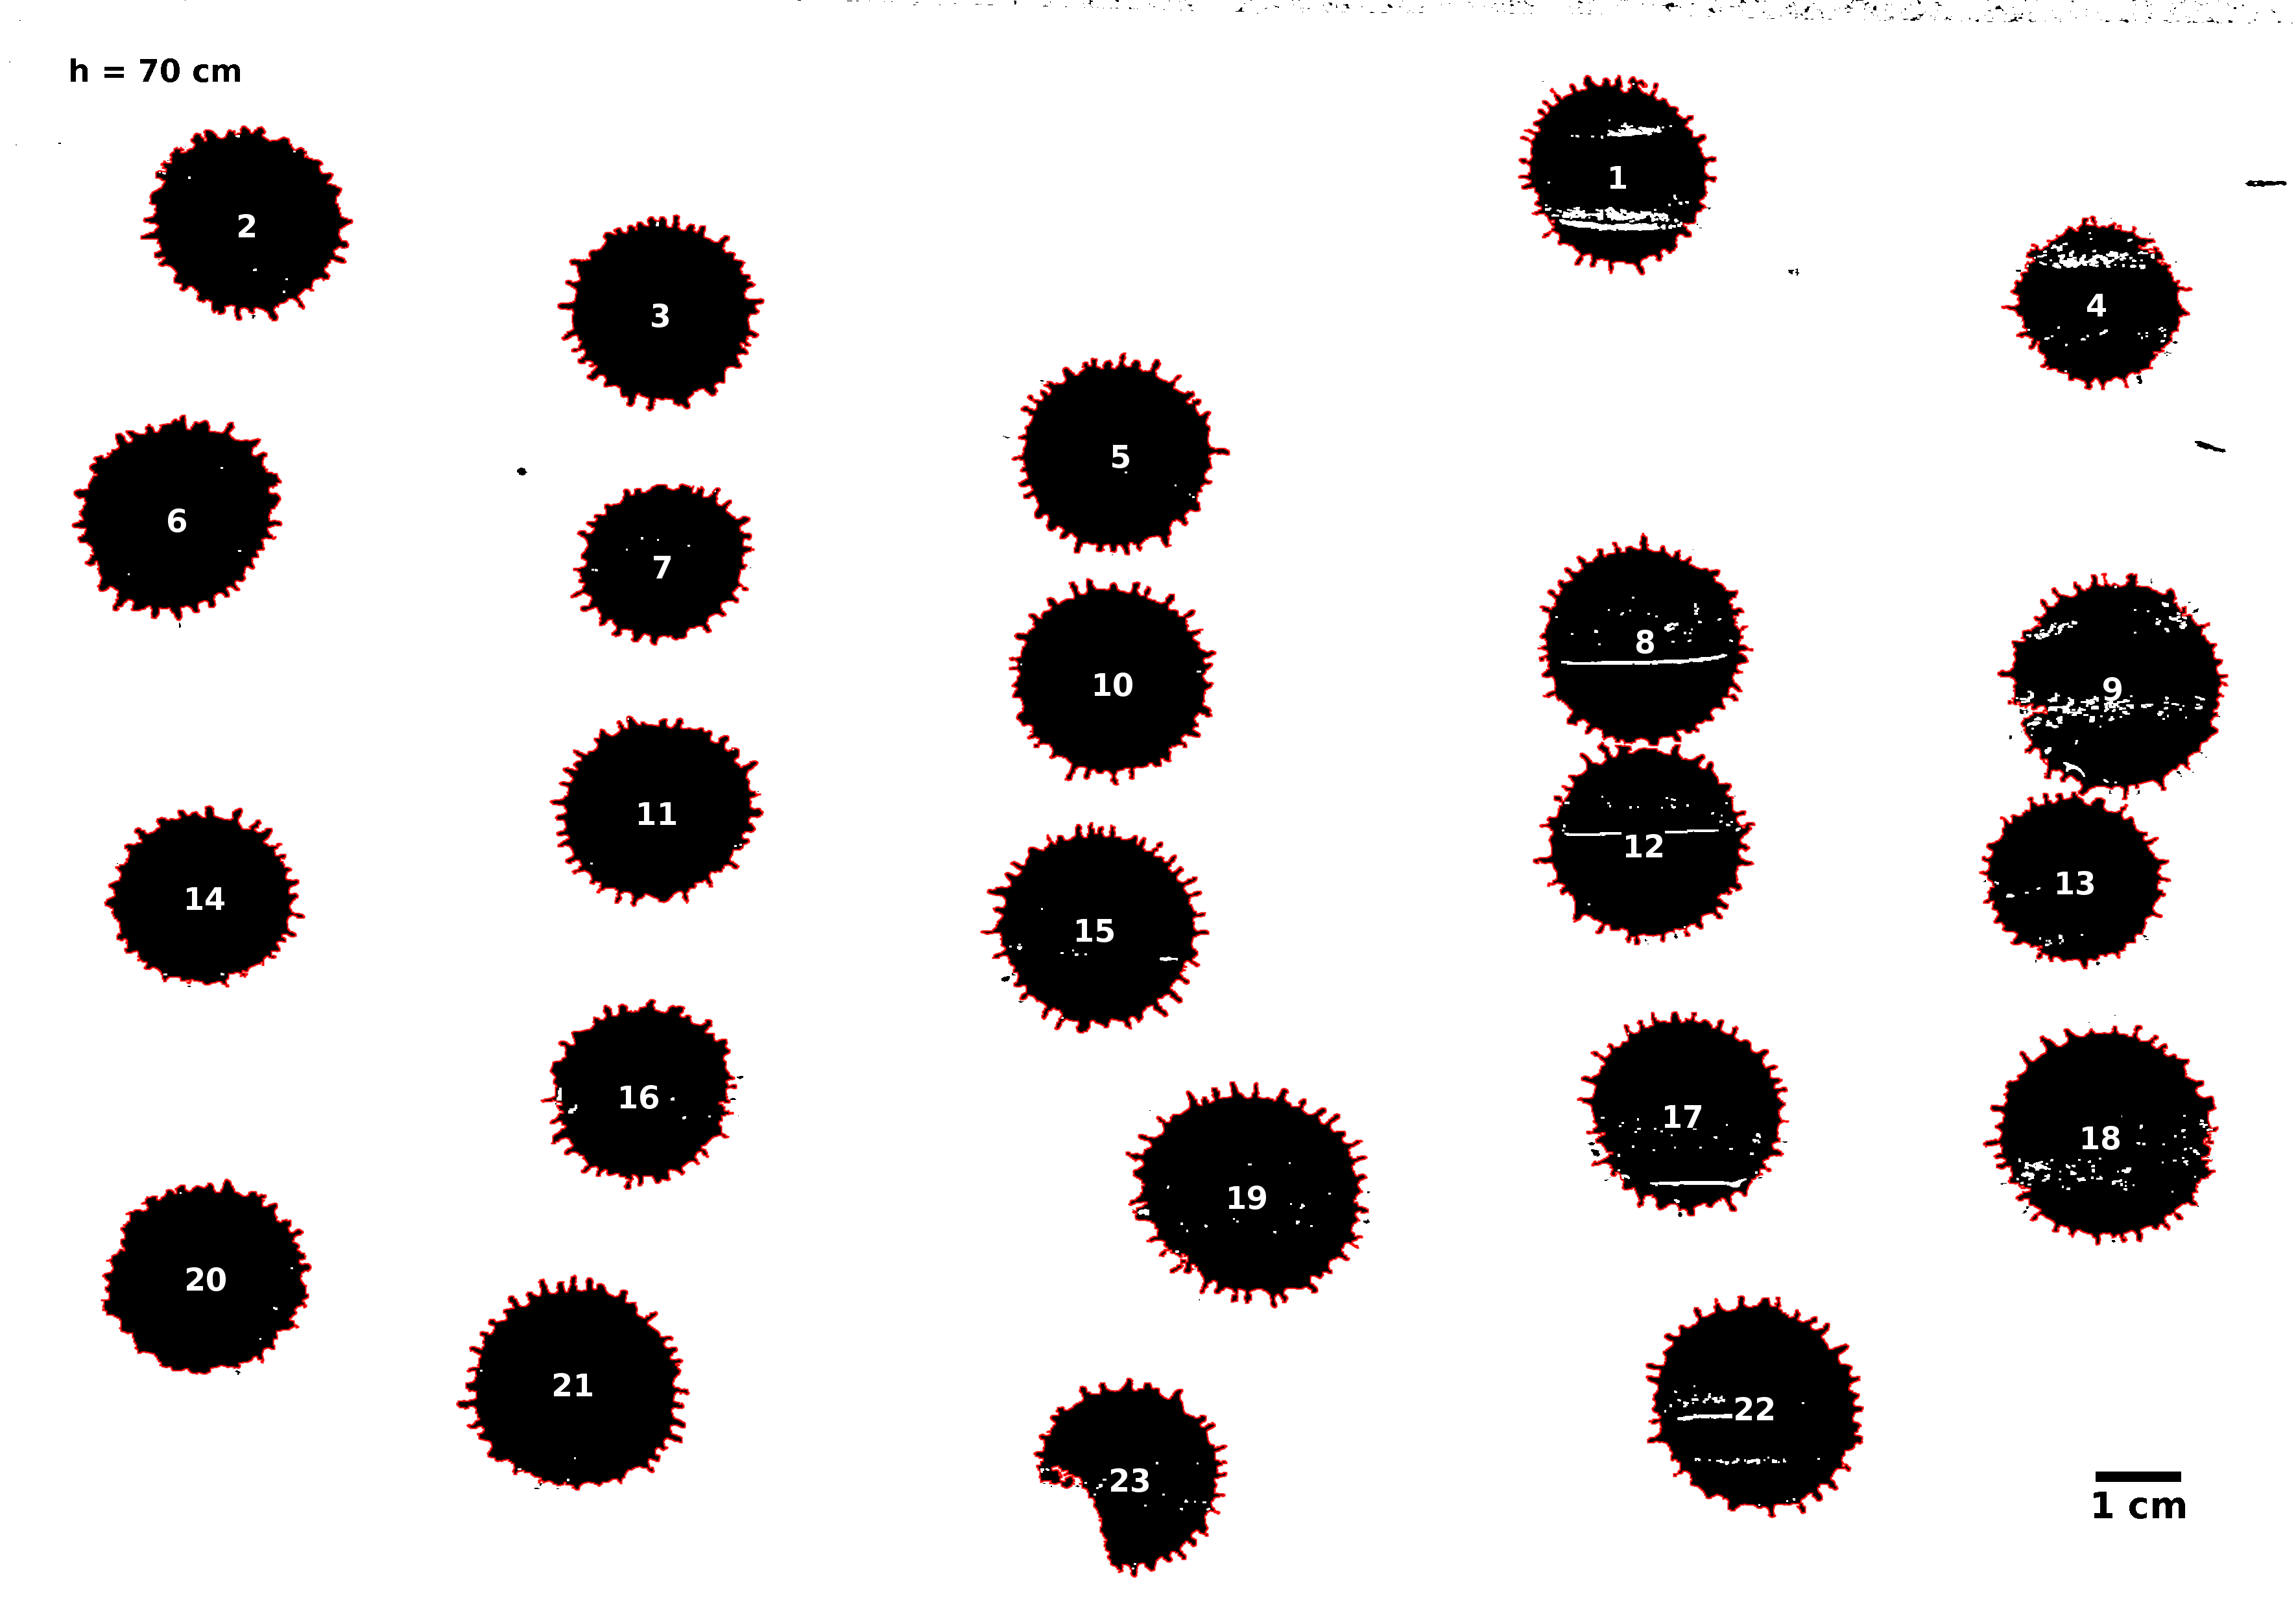
\includegraphics[width=0.75\linewidth]{src/70-1.png} \caption{Mancha de gotas
desde $70\ cm$} \label{fig:70cm-1} \end{figure}

\begin{table}[H] \centering \caption{Datos obtenidos a partir de la figura
    ~\ref{fig:80cm-1} ($h=80\ cm)$} \label{tab:80cm} \begin{tabular}{cccccc}
        \toprule Gota & Área ($cm^2$) & Perímetro ($cm$) & Eje mayor ($cm$) &
        Eje menor ($cm$) & Dirección ($^o$) \\ \midrule 1  & 4.34 & 18.81 &
        2.42 & 2.28 & 177.44 \\ 2  & 3.82 & 14.46 & 2.32 & 2.09 & 42.73  \\ 3
             & 3.63 & 13.57 & 2.24 & 2.07 & 157.73 \\ 4  & 4.05 & 15.45 & 2.39
             & 2.16 & 44.30  \\ 5  & 4.29 & 13.64 & 2.40 & 2.28 & 167.56 \\ 6
             & 4.15 & 14.05 & 2.36 & 2.24 & 39.91  \\ 7  & 3.85 & 12.35 & 2.31
             & 2.12 & 48.42  \\ 8  & 4.61 & 15.77 & 2.48 & 2.37 & 38.43  \\ 9
             & 3.92 & 16.11 & 2.30 & 2.17 & 53.45  \\ 10 & 4.15 & 14.39 & 2.33
             & 2.27 & 171.79 \\ 11 & 4.13 & 15.05 & 2.40 & 2.20 & 143.39 \\ 12
             & 3.95 & 12.51 & 2.29 & 2.20 & 151.58 \\ 13 & 4.34 & 15.86 & 2.43
             & 2.28 & 36.40  \\ 14 & 4.55 & 15.30 & 2.44 & 2.37 & 14.26  \\ 15
             & 3.54 & 13.58 & 2.20 & 2.05 & 50.57  \\ 16 & 4.06 & 15.91 & 2.38
             & 2.17 & 56.51  \\ 17 & 4.21 & 13.77 & 2.42 & 2.22 & 4.25   \\
        \midrule Media & 4.09 & 14.74 & 2.36 & 2.21 & 82.28 \\ \bottomrule
    \end{tabular} \end{table}

\begin{figure}[H] \centering
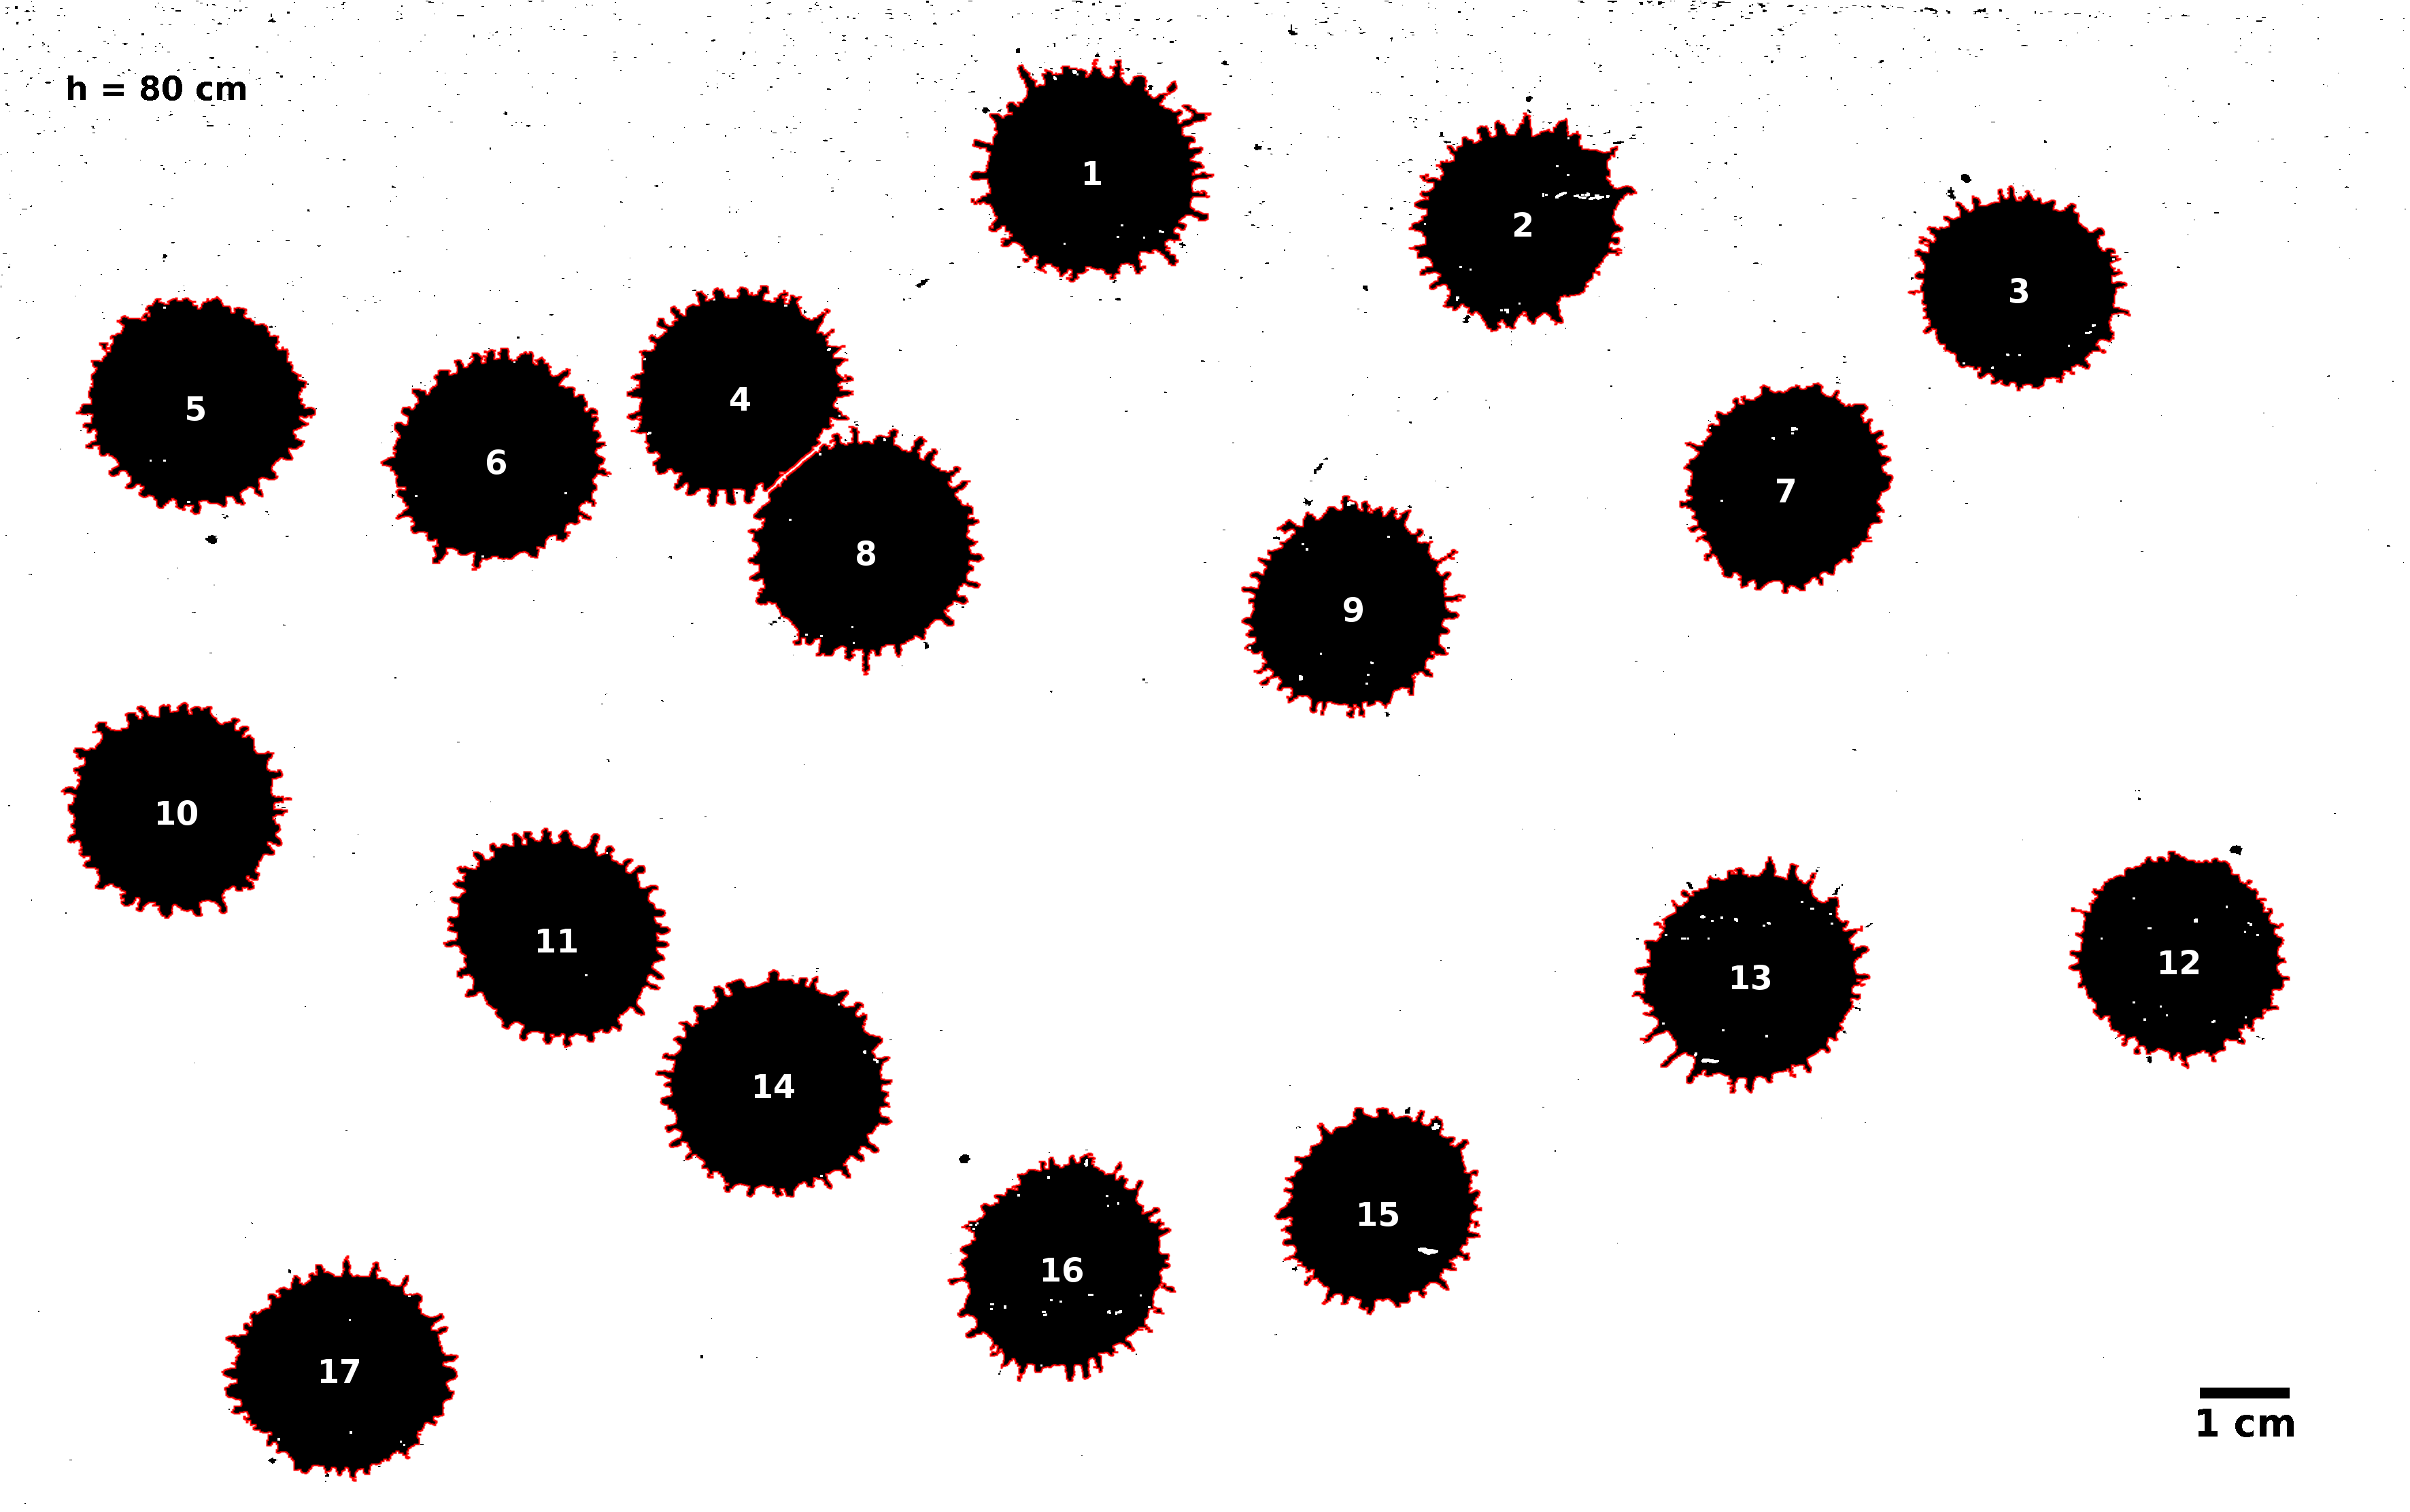
\includegraphics[width=0.85\linewidth]{src/80-1.png} \caption{Mancha de gotas
desde $80\ cm$} \label{fig:80cm-1} \end{figure}

\begin{table}[H] \centering \caption{Datos obtenidos a partir de la figura
    ~\ref{fig:90cm-1} ($h=90\ cm)$} \label{tab:90cm} \begin{tabular}{cccccc}
        \toprule Gota & Área ($cm^2$) & Perímetro ($cm$) & Eje mayor ($cm$) &
        Eje menor ($cm$) & Dirección ($^o$) \\ \midrule 1  & 4.57 & 18.80 &
        2.46 & 2.37 & 116.67 \\ 2  & 3.80 & 14.87 & 2.28 & 2.13 & 41.77  \\ 3
             & 3.92 & 13.70 & 2.29 & 2.18 & 14.94  \\ 4  & 4.47 & 17.47 & 2.46
             & 2.31 & 157.72 \\ 5  & 3.81 & 12.18 & 2.27 & 2.14 & 43.38  \\ 6
             & 4.22 & 15.60 & 2.39 & 2.25 & 42.62  \\ 7  & 4.52 & 15.48 & 2.47
             & 2.33 & 9.79   \\ 8  & 4.37 & 15.57 & 2.45 & 2.27 & 46.43  \\ 9
             & 4.46 & 17.77 & 2.54 & 2.23 & 155.31 \\ 10 & 4.70 & 15.47 & 2.50
             & 2.39 & 10.91  \\ 11 & 4.30 & 13.10 & 2.44 & 2.25 & 141.63 \\ 12
             & 4.26 & 15.31 & 2.37 & 2.29 & 172.27 \\ 13 & 4.06 & 17.03 & 2.37
             & 2.18 & 140.85 \\ 14 & 3.99 & 13.02 & 2.30 & 2.21 & 145.33 \\ 15
             & 5.20 & 18.62 & 2.62 & 2.52 & 22.10  \\ 16 & 3.91 & 12.70 & 2.25
             & 2.21 & 155.09 \\ 17 & 4.77 & 16.48 & 2.52 & 2.41 & 17.41  \\ 18
             & 3.86 & 14.94 & 2.29 & 2.14 & 53.27  \\ 19 & 4.51 & 17.67 & 2.43
             & 2.37 & 117.64 \\ 20 & 4.53 & 15.49 & 2.42 & 2.39 & 16.31  \\
    \midrule Media & 4.31 & 15.56 & 2.41 & 2.28 & 81.07  \\ \bottomrule
\end{tabular} \end{table}

\begin{figure}[H] \centering
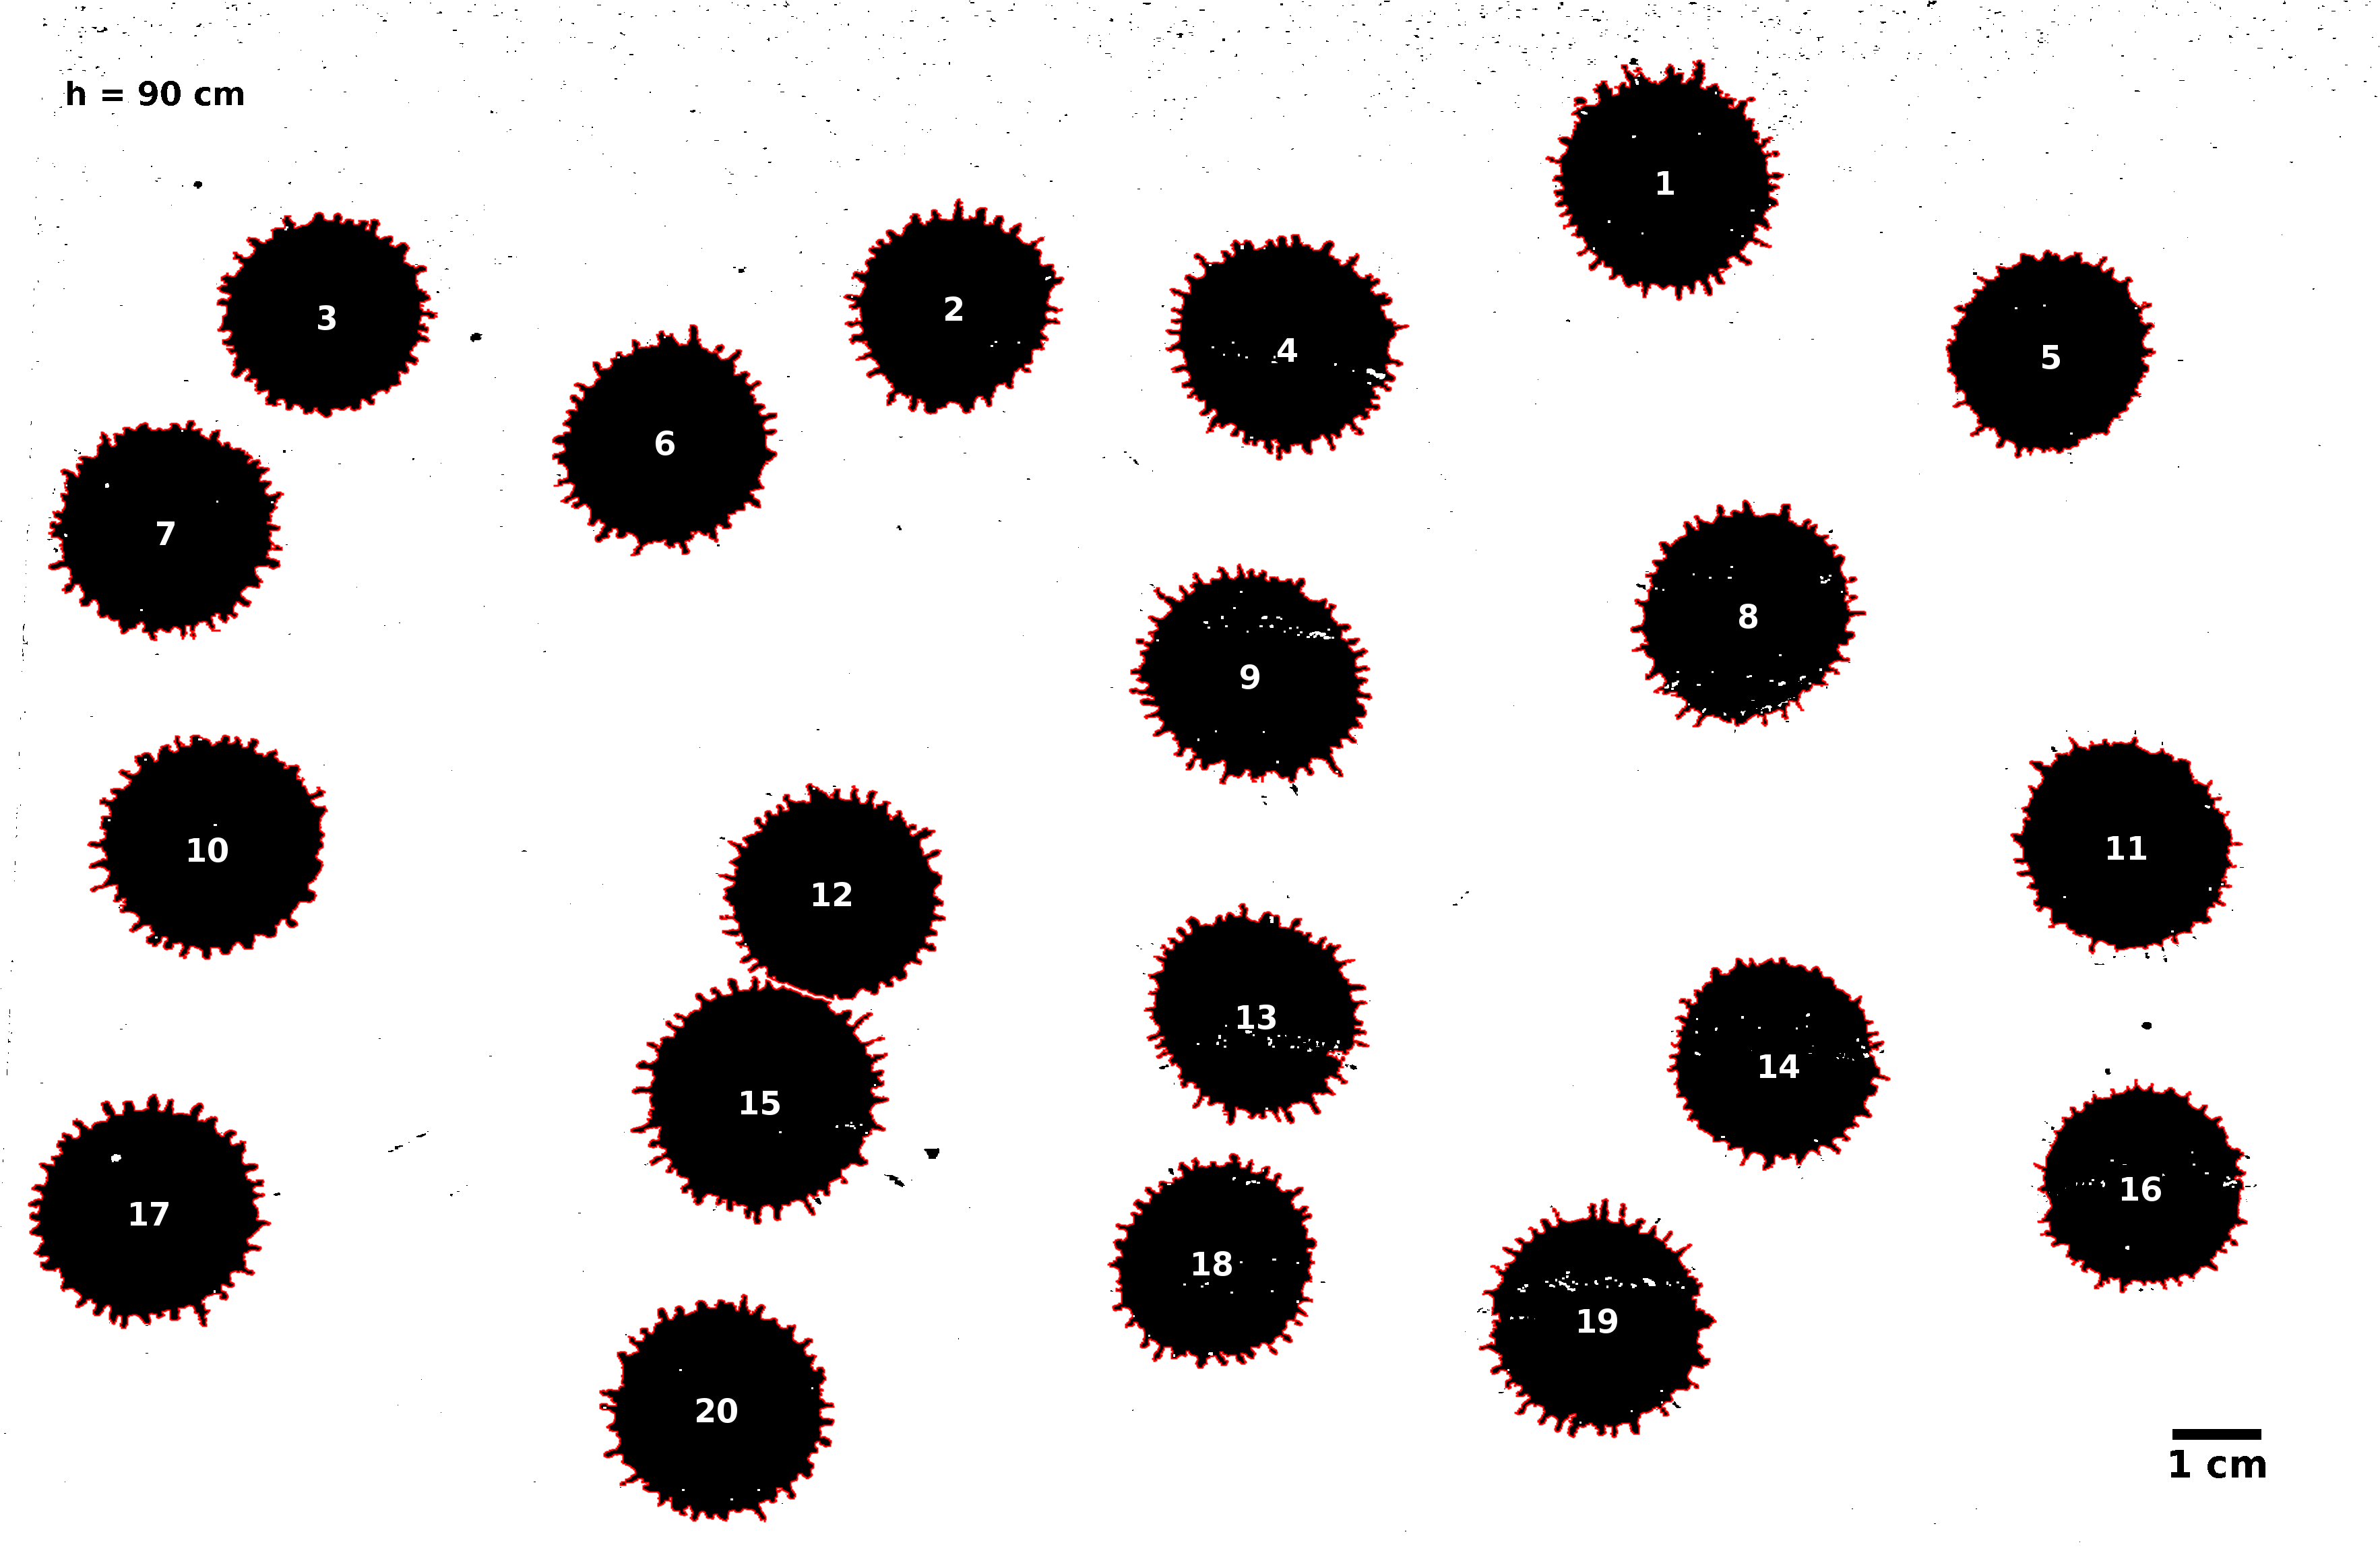
\includegraphics[width=0.85\linewidth]{src/90-1.png} \caption{Mancha de gotas
desde $90\ cm$} \label{fig:90cm-1} \end{figure}

\begin{table}[H] \centering \caption{Datos obtenidos a partir de la figura
    ~\ref{fig:100-1} ($h=100\ cm)$} \label{tab:100} \begin{tabular}{cccccc}
        \toprule Gota & Área ($cm^2$) & Perímetro ($cm$) & Eje mayor ($cm$) &
        Eje menor ($cm$) & Dirección ($^o$) \\ \midrule 1  & 4.72 & 19.64 &
        2.61 & 2.30 & 11.96  \\ 2  & 4.14 & 15.67 & 2.46 & 2.14 & 156.61 \\ 3
             & 4.62 & 15.22 & 2.56 & 2.29 & 136.65 \\ 4  & 4.70 & 15.83 & 2.50
             & 2.39 & 175.36 \\ 5  & 4.75 & 19.43 & 2.69 & 2.25 & 147.23 \\ 6
             & 4.12 & 17.65 & 2.37 & 2.21 & 15.10  \\ 7  & 5.18 & 19.88 & 2.70
             & 2.44 & 53.69  \\ 8  & 3.70 & 16.00 & 2.19 & 2.15 & 169.90 \\ 9
             & 4.18 & 16.78 & 2.44 & 2.18 & 152.60 \\ 10 & 6.06 & 19.56 & 2.84
             & 2.72 & 21.04  \\ 11 & 4.61 & 17.24 & 2.49 & 2.36 & 66.54  \\ 12
             & 6.02 & 20.09 & 2.87 & 2.68 & 151.57 \\ 13 & 4.66 & 18.43 & 2.51
             & 2.37 & 143.10 \\ 14 & 4.60 & 16.78 & 2.53 & 2.31 & 117.92 \\
    \midrule Media & 4.72 & 17.73 & 2.55 & 2.34 & 108.52 \\ \bottomrule
\end{tabular} \end{table}

\begin{figure}[H] \centering
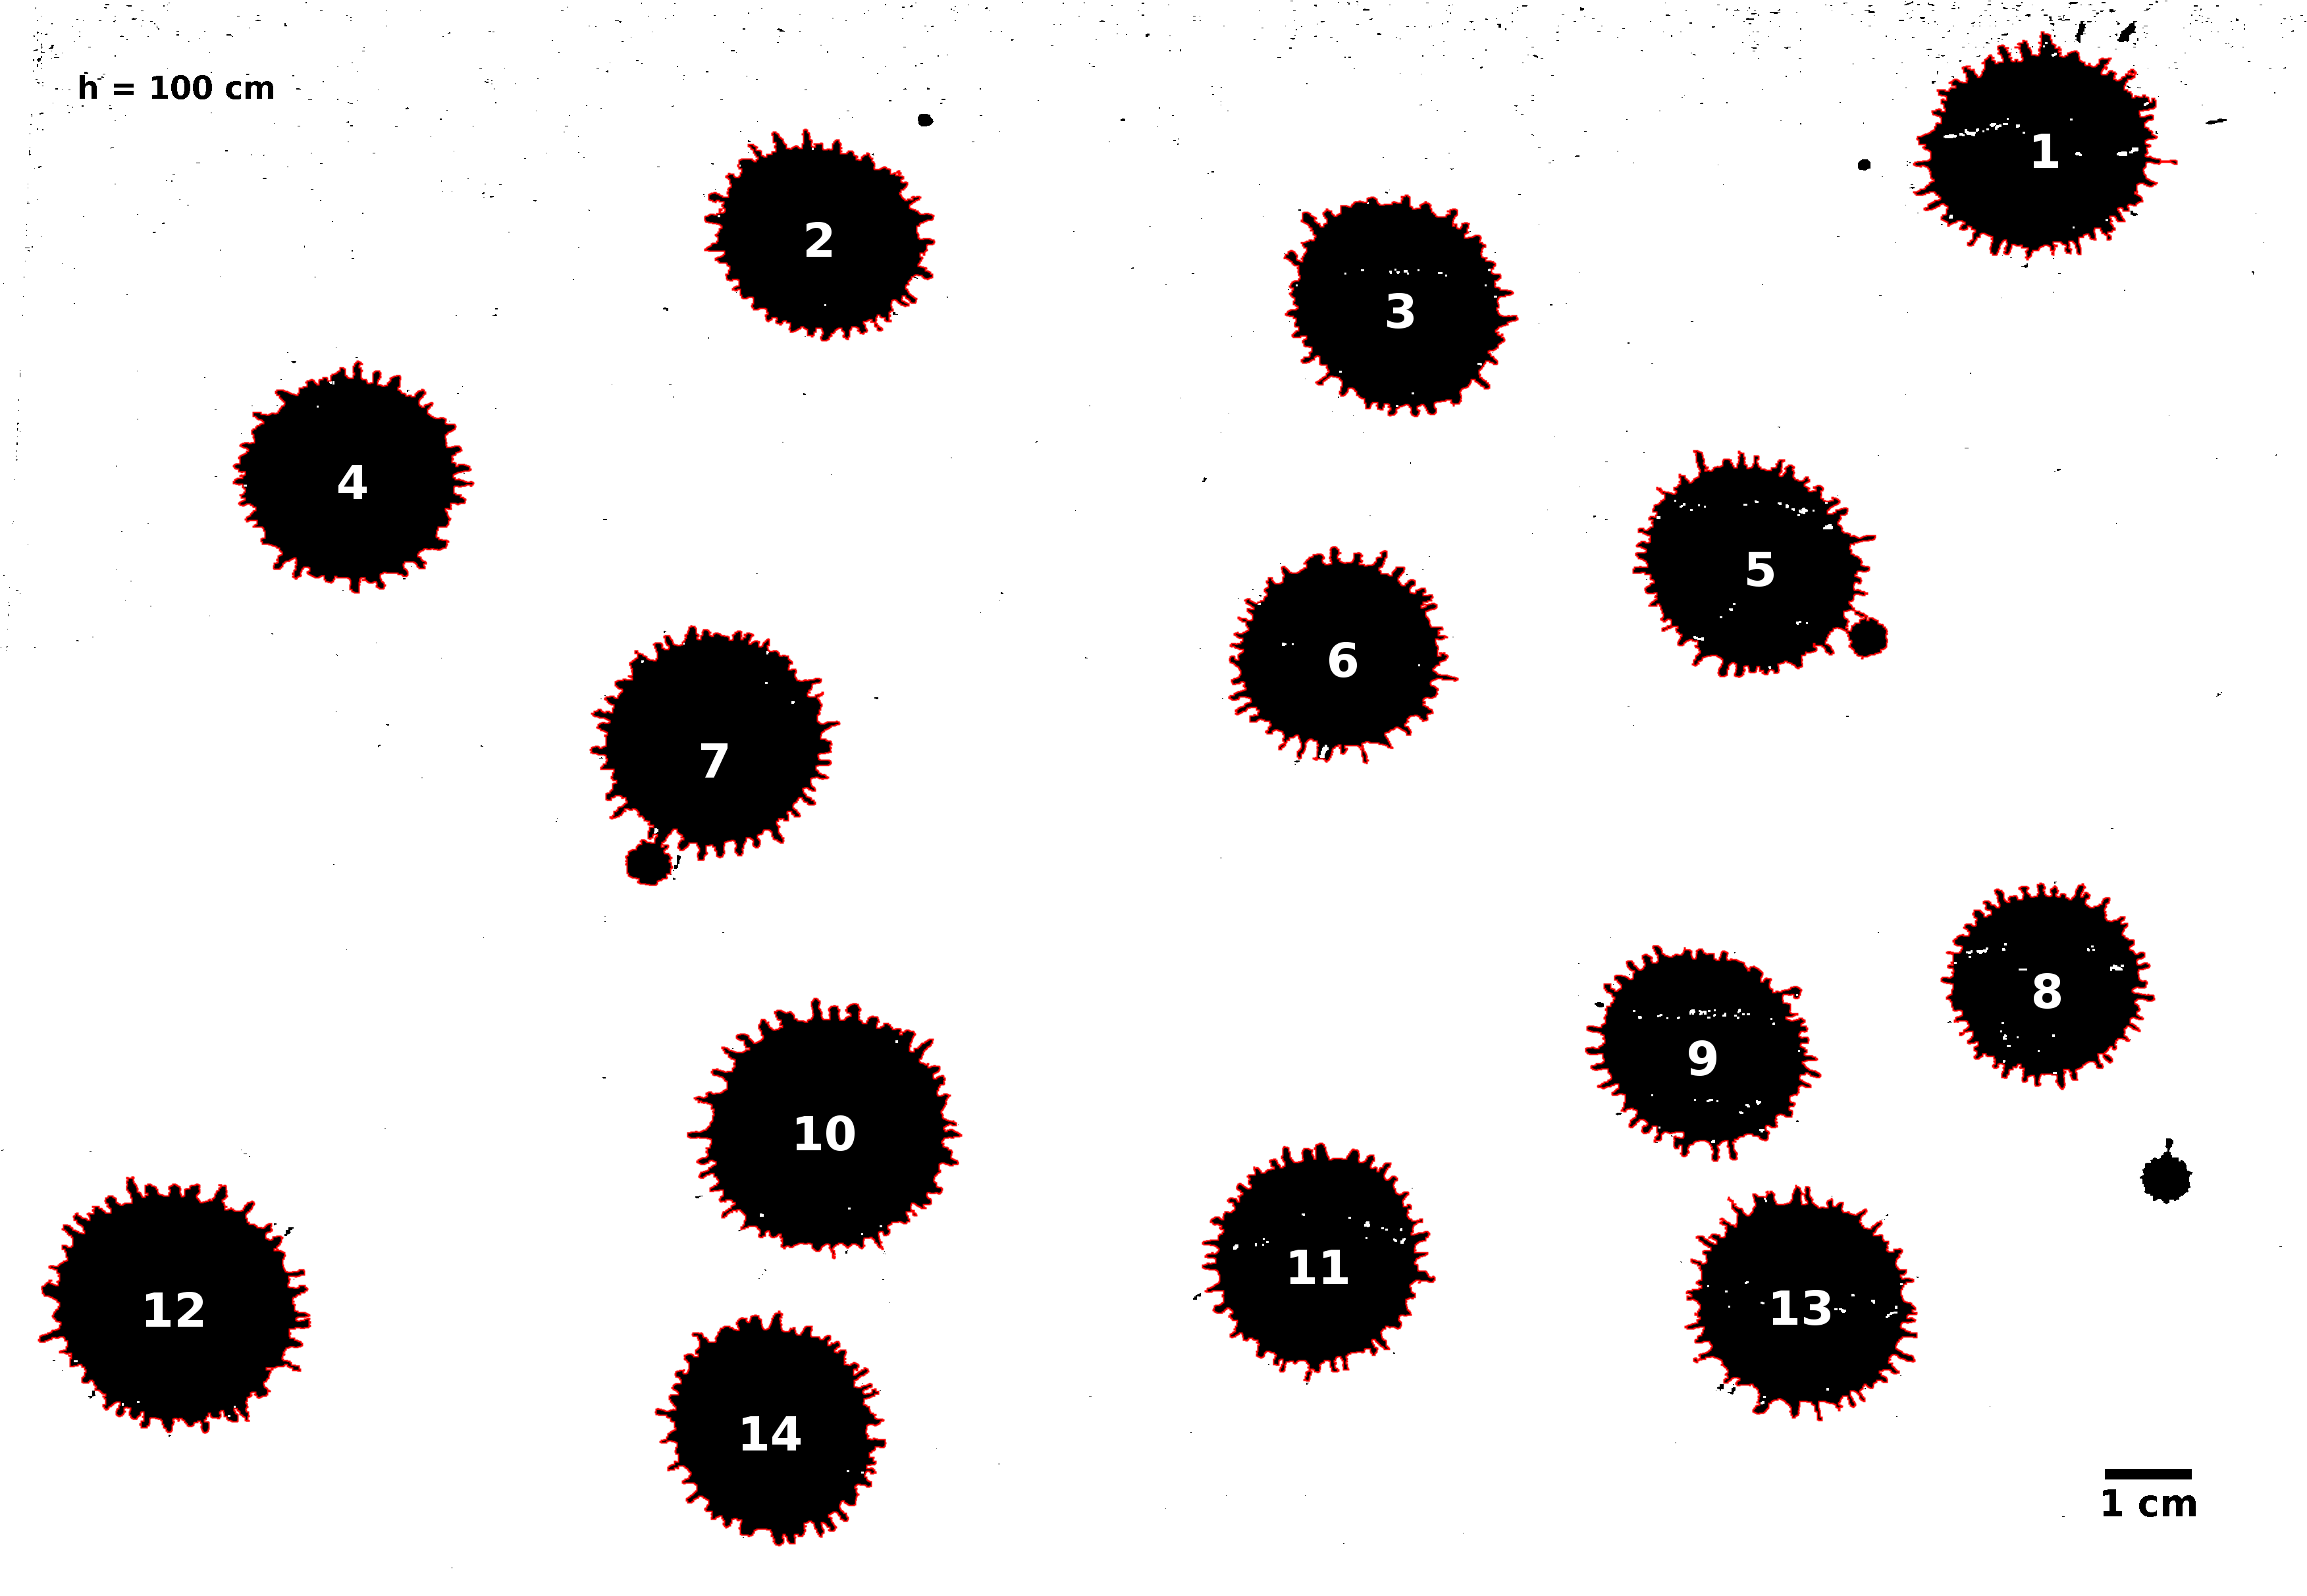
\includegraphics[width=0.90\linewidth]{src/100-1.png} \caption{Mancha de gotas
desde $100\ cm$} \label{fig:100-1} \end{figure}

\pagebreak \subsection{Experimento 2} \label{sub:experimento_2}

\begin{table}[H] \centering \caption{Datos obtenidos a partir de la figura
    ~\ref{fig:15deg-1} ($\alpha=15^o)$} \label{tab:15deg}
    \begin{tabular}{cccccc} \toprule Gota & Área ($cm^2$) & Perímetro ($cm$) &
        Eje mayor ($cm$) & Eje menor ($cm$) & Dirección ($^o$) \\ \midrule 1  &
        4.33 & 9.66  & 2.38 & 2.32 & 163.36 \\ 2  & 2.68 & 8.43  & 1.87 & 1.82
             & 158.93 \\ 3  & 4.45 & 10.53 & 2.44 & 2.32 & 172.27 \\ 4  & 3.52
             & 9.79  & 2.28 & 1.96 & 12.8   \\ 5  & 3.1  & 8.12  & 2.09 & 1.89
             & 14.36  \\ 6  & 4.84 & 11.56 & 2.67 & 2.31 & 1.74   \\ 7  & 4.07
             & 10.74 & 2.35 & 2.2  & 16.97  \\ 8  & 4.72 & 10.31 & 2.56 & 2.35
             & 1.45   \\ 9  & 4.71 & 10.97 & 2.58 & 2.33 & 1.75   \\ 10 & 3.55
             & 8.97  & 2.21 & 2.04 & 173.2  \\ 11 & 4.02 & 9.38  & 2.38 & 2.15
             & 163.1  \\ 12 & 4.16 & 9.18  & 2.31 & 2.29 & 98.69  \\ \midrule
        Media & 4.01 & 9.80  & 2.34 & 2.17 & 81.55 \\ \bottomrule \end{tabular}
    \end{table}

\begin{figure}[H] \centering
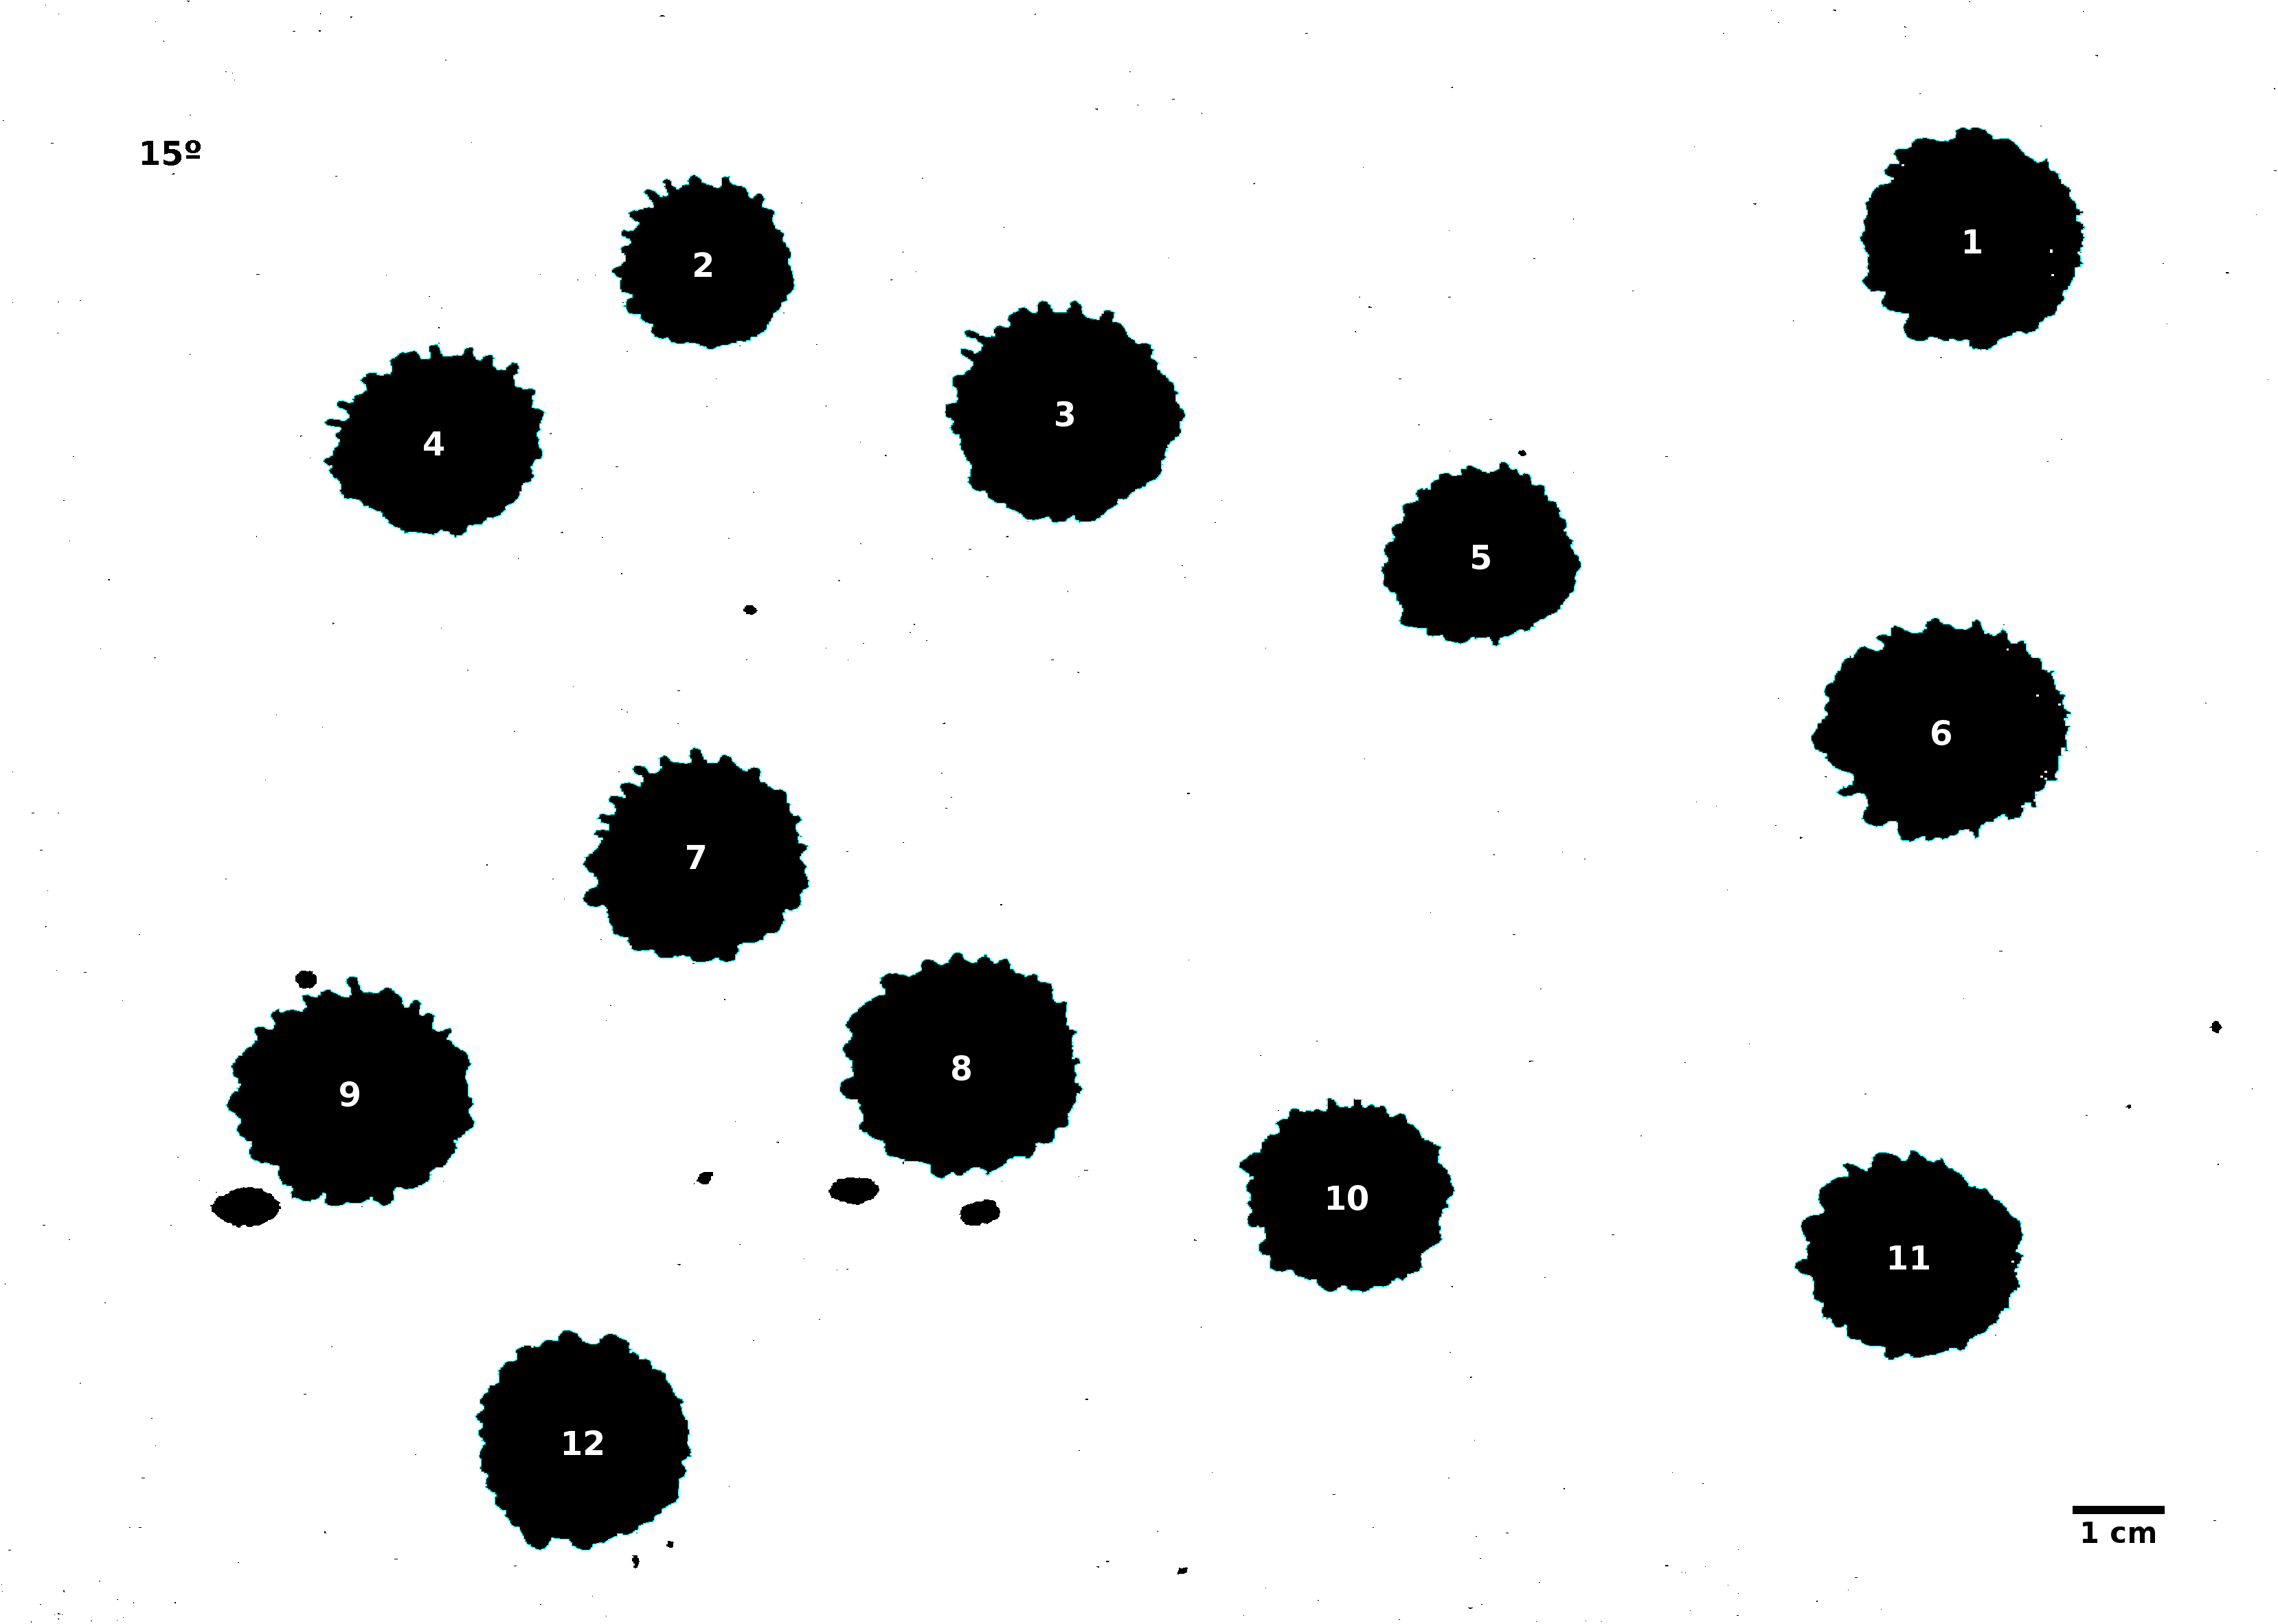
\includegraphics[width=0.66\linewidth]{src/15_deg-1.png} \caption{Mancha de
gotas sobre plano inclinado $15^o$} \label{fig:15deg-1} \end{figure}

\begin{table}[H] \centering \caption{Datos obtenidos a partir de la figura
    ~\ref{fig:30deg-1} ($\alpha=30^o)$} \label{tab:30deg}
    \begin{tabular}{cccccc} \toprule Gota & Área ($cm^2$) & Perímetro ($cm$) &
        Eje mayor ($cm$) & Eje menor ($cm$) & Dirección ($^o$) \\ \midrule 1  &
        5.2  & 13.31 & 2.66 & 2.49 & 12.57  \\ 2  & 4.29 & 12.56 & 2.45 & 2.23
             & 3.41   \\ 3  & 4.02 & 11.95 & 2.58 & 1.98 & 3.42   \\ 4  & 4.05
             & 11.67 & 2.34 & 2.2  & 174.81 \\ 5  & 4.13 & 12.16 & 2.42 & 2.17
             & 171.12 \\ 6  & 4.01 & 11.75 & 2.5  & 2.04 & 163.46 \\ 7  & 4.9
             & 13.39 & 2.77 & 2.25 & 23.62  \\ 8  & 4.15 & 13.2  & 2.58 & 2.05
             & 173.84 \\ 9  & 4.46 & 12.32 & 2.58 & 2.2  & 149.62 \\ 10 & 5.9
             & 15.15 & 3.21 & 2.34 & 178.33 \\ 11 & 4.03 & 11.81 & 2.52 & 2.04
             & 10.14  \\ 12 & 3.98 & 11.28 & 2.48 & 2.04 & 13.59  \\ 13 & 4.39
             & 13.15 & 2.53 & 2.21 & 167.4  \\ 14 & 4.77 & 11.71 & 2.52 & 2.41
             & 177.13 \\ 15 & 4.59 & 10.97 & 2.69 & 2.17 & 3.77   \\ \midrule
    Media & 4.45 & 12.53 & 2.58 & 2.19 & 101.60 \\ \bottomrule \end{tabular}
\end{table}

\begin{figure}[H] \centering
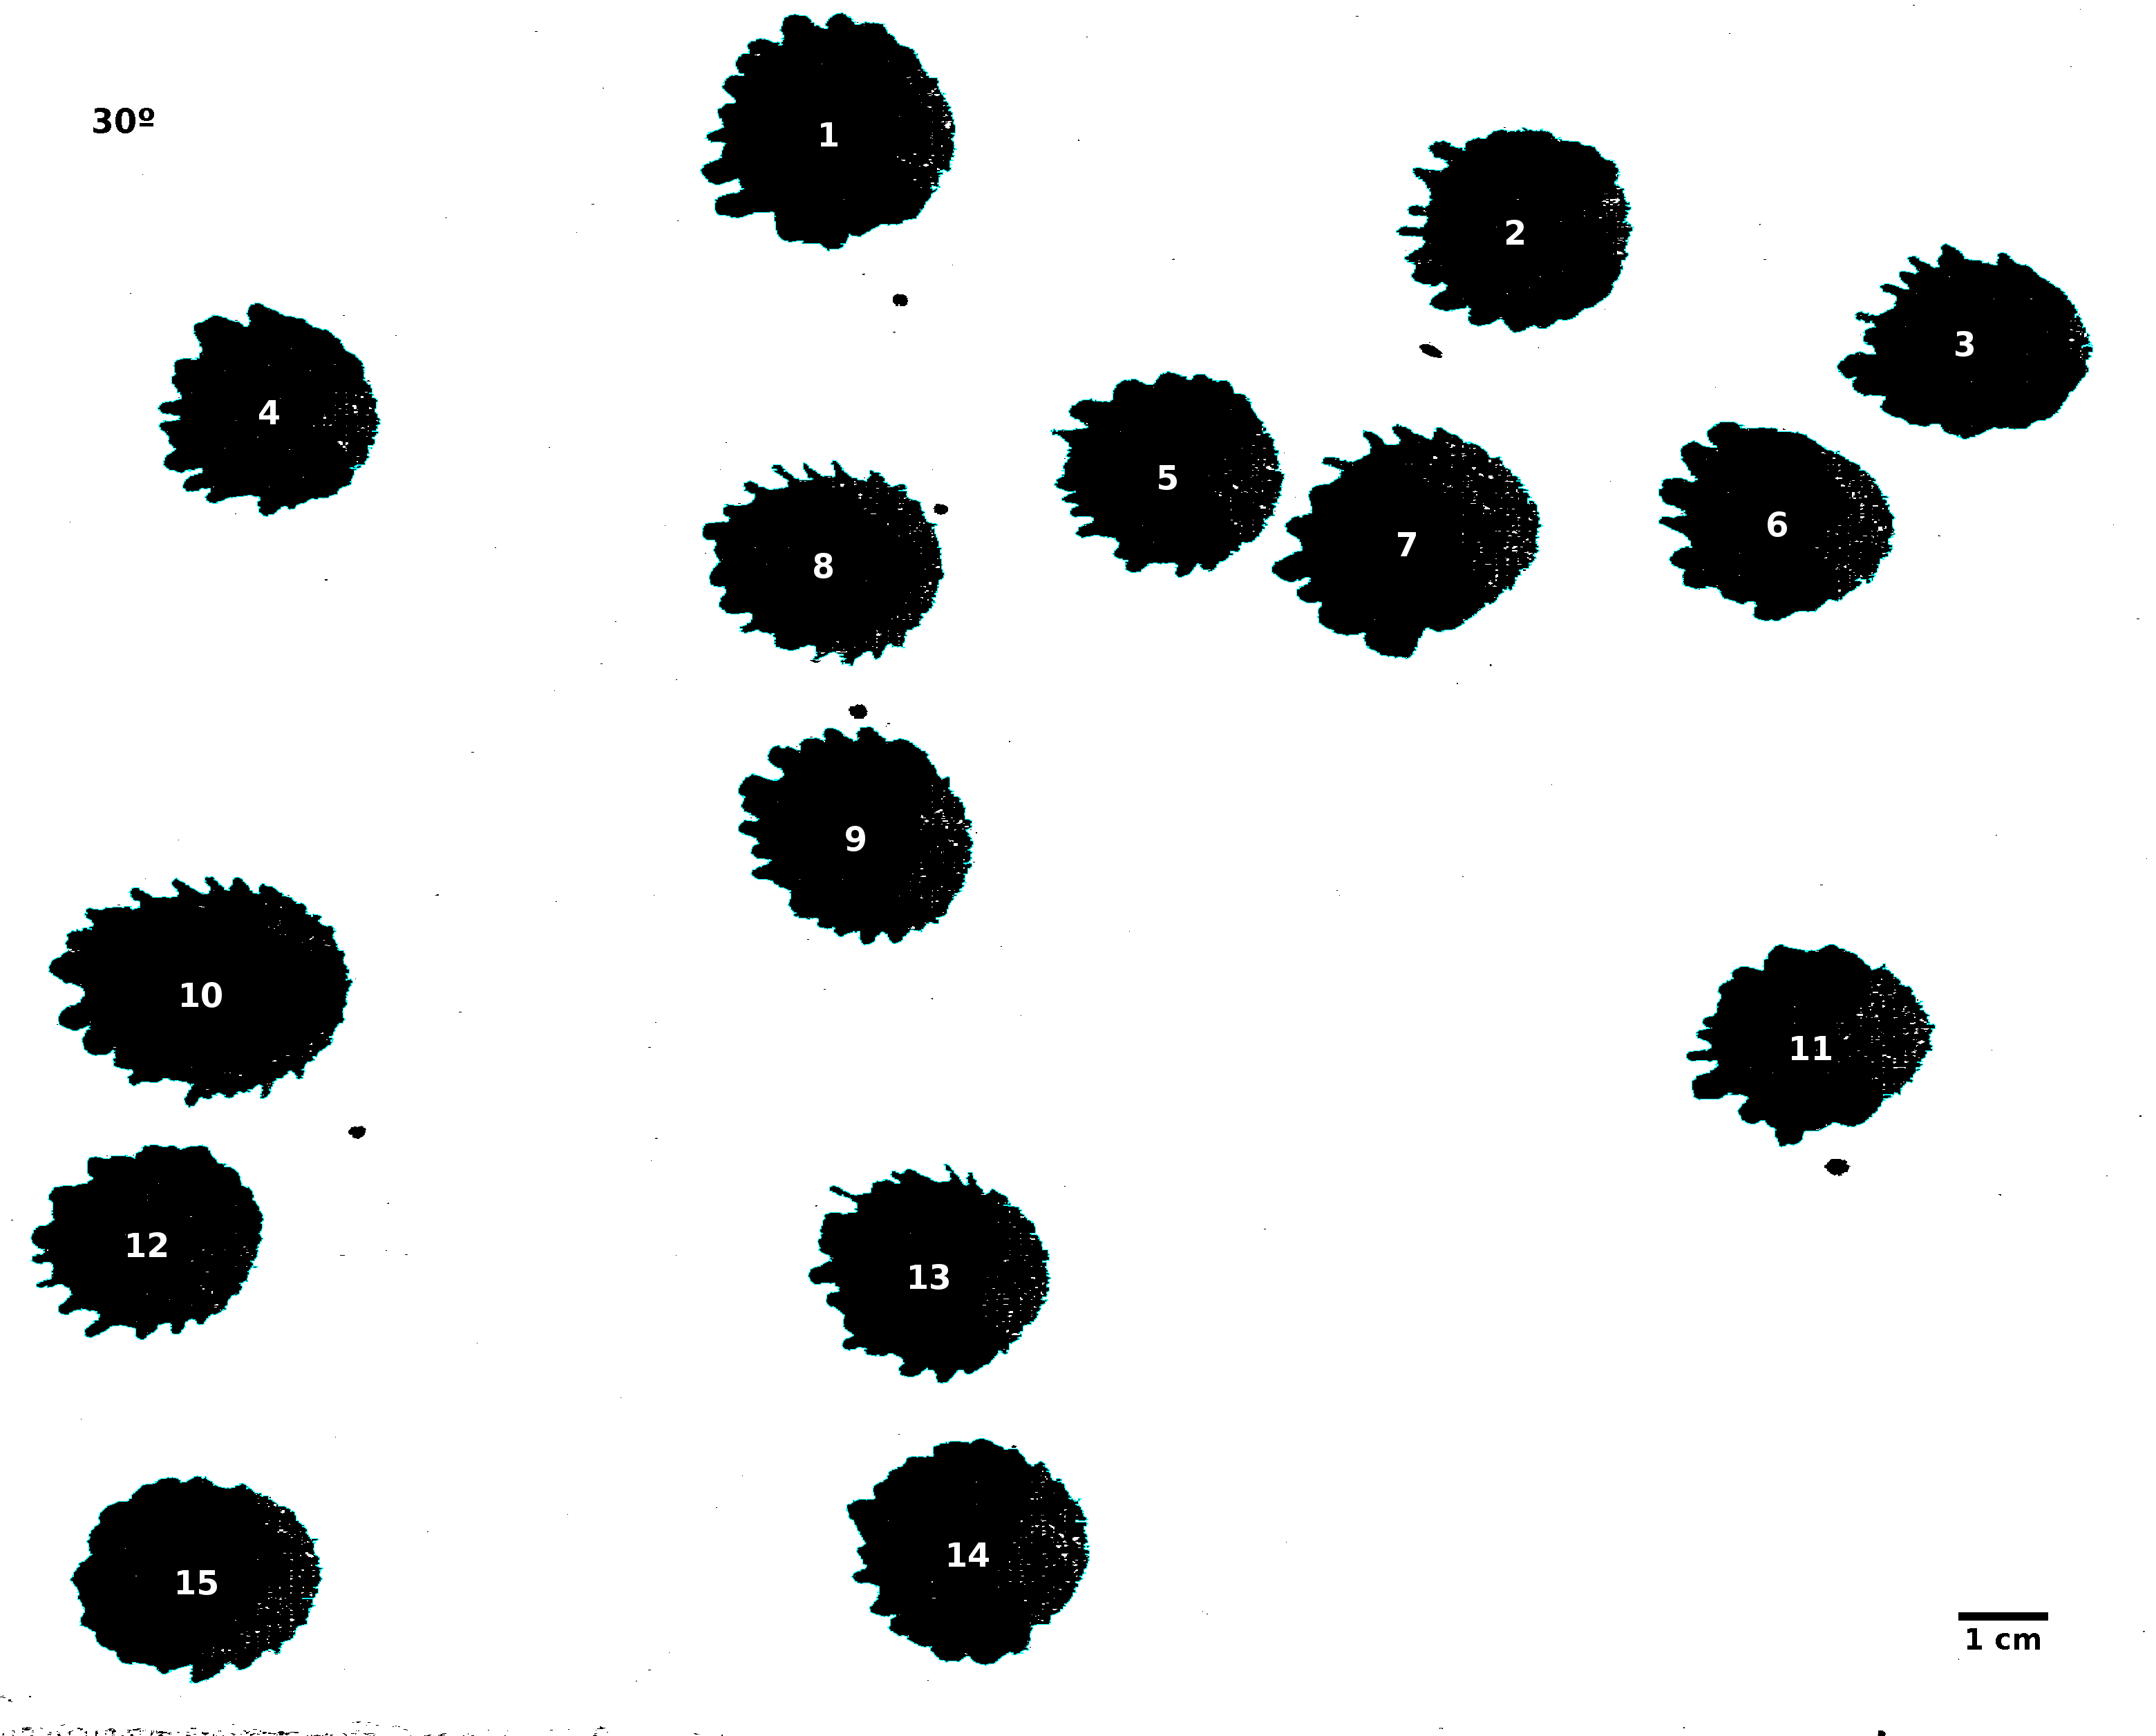
\includegraphics[width=0.66\linewidth]{src/30_deg-1.png} \caption{Mancha de
gotas sobre plano inclinado $30^o$} \label{fig:30deg-1} \end{figure}

\begin{table}[H] \centering \caption{Datos obtenidos a partir de la figura
    ~\ref{fig:45deg-1} ($\alpha=45^o)$} \label{tab:45deg}
    \begin{tabular}{cccccc} \toprule Gota & Área ($cm^2$) & Perímetro ($cm$) &
        Eje mayor ($cm$) & Eje menor ($cm$) & Dirección ($^o$) \\ \midrule 1
                         & 4.58 & 11.77 & 3.34 & 1.75 & 172.99 \\ 2     & 4.74
                         & 12.98 & 2.97 & 2.03 & 178.92 \\ 3     & 5.56 & 16.10
                         & 3.18 & 2.22 & 2.11   \\ 4     & 5.51 & 15.08 & 3.23
                         & 2.17 & 177.29 \\ 5     & 5.00 & 13.71 & 3.14 & 2.03
                         & 176.35 \\ 6     & 5.13 & 13.63 & 3.28 & 1.99 & 1.60
        \\ 7     & 6.05 & 17.35 & 3.57 & 2.16 & 3.37   \\ 8     & 5.64 & 14.79
                 & 3.41 & 2.11 & 0.75   \\ 9     & 6.24 & 14.61 & 3.43 & 2.32 &
        8.27   \\ \midrule Media & 5.38 & 14.45 & 3.28 & 2.09 & 80.18 \\
    \bottomrule \end{tabular} \end{table}

\begin{figure}[H] \centering
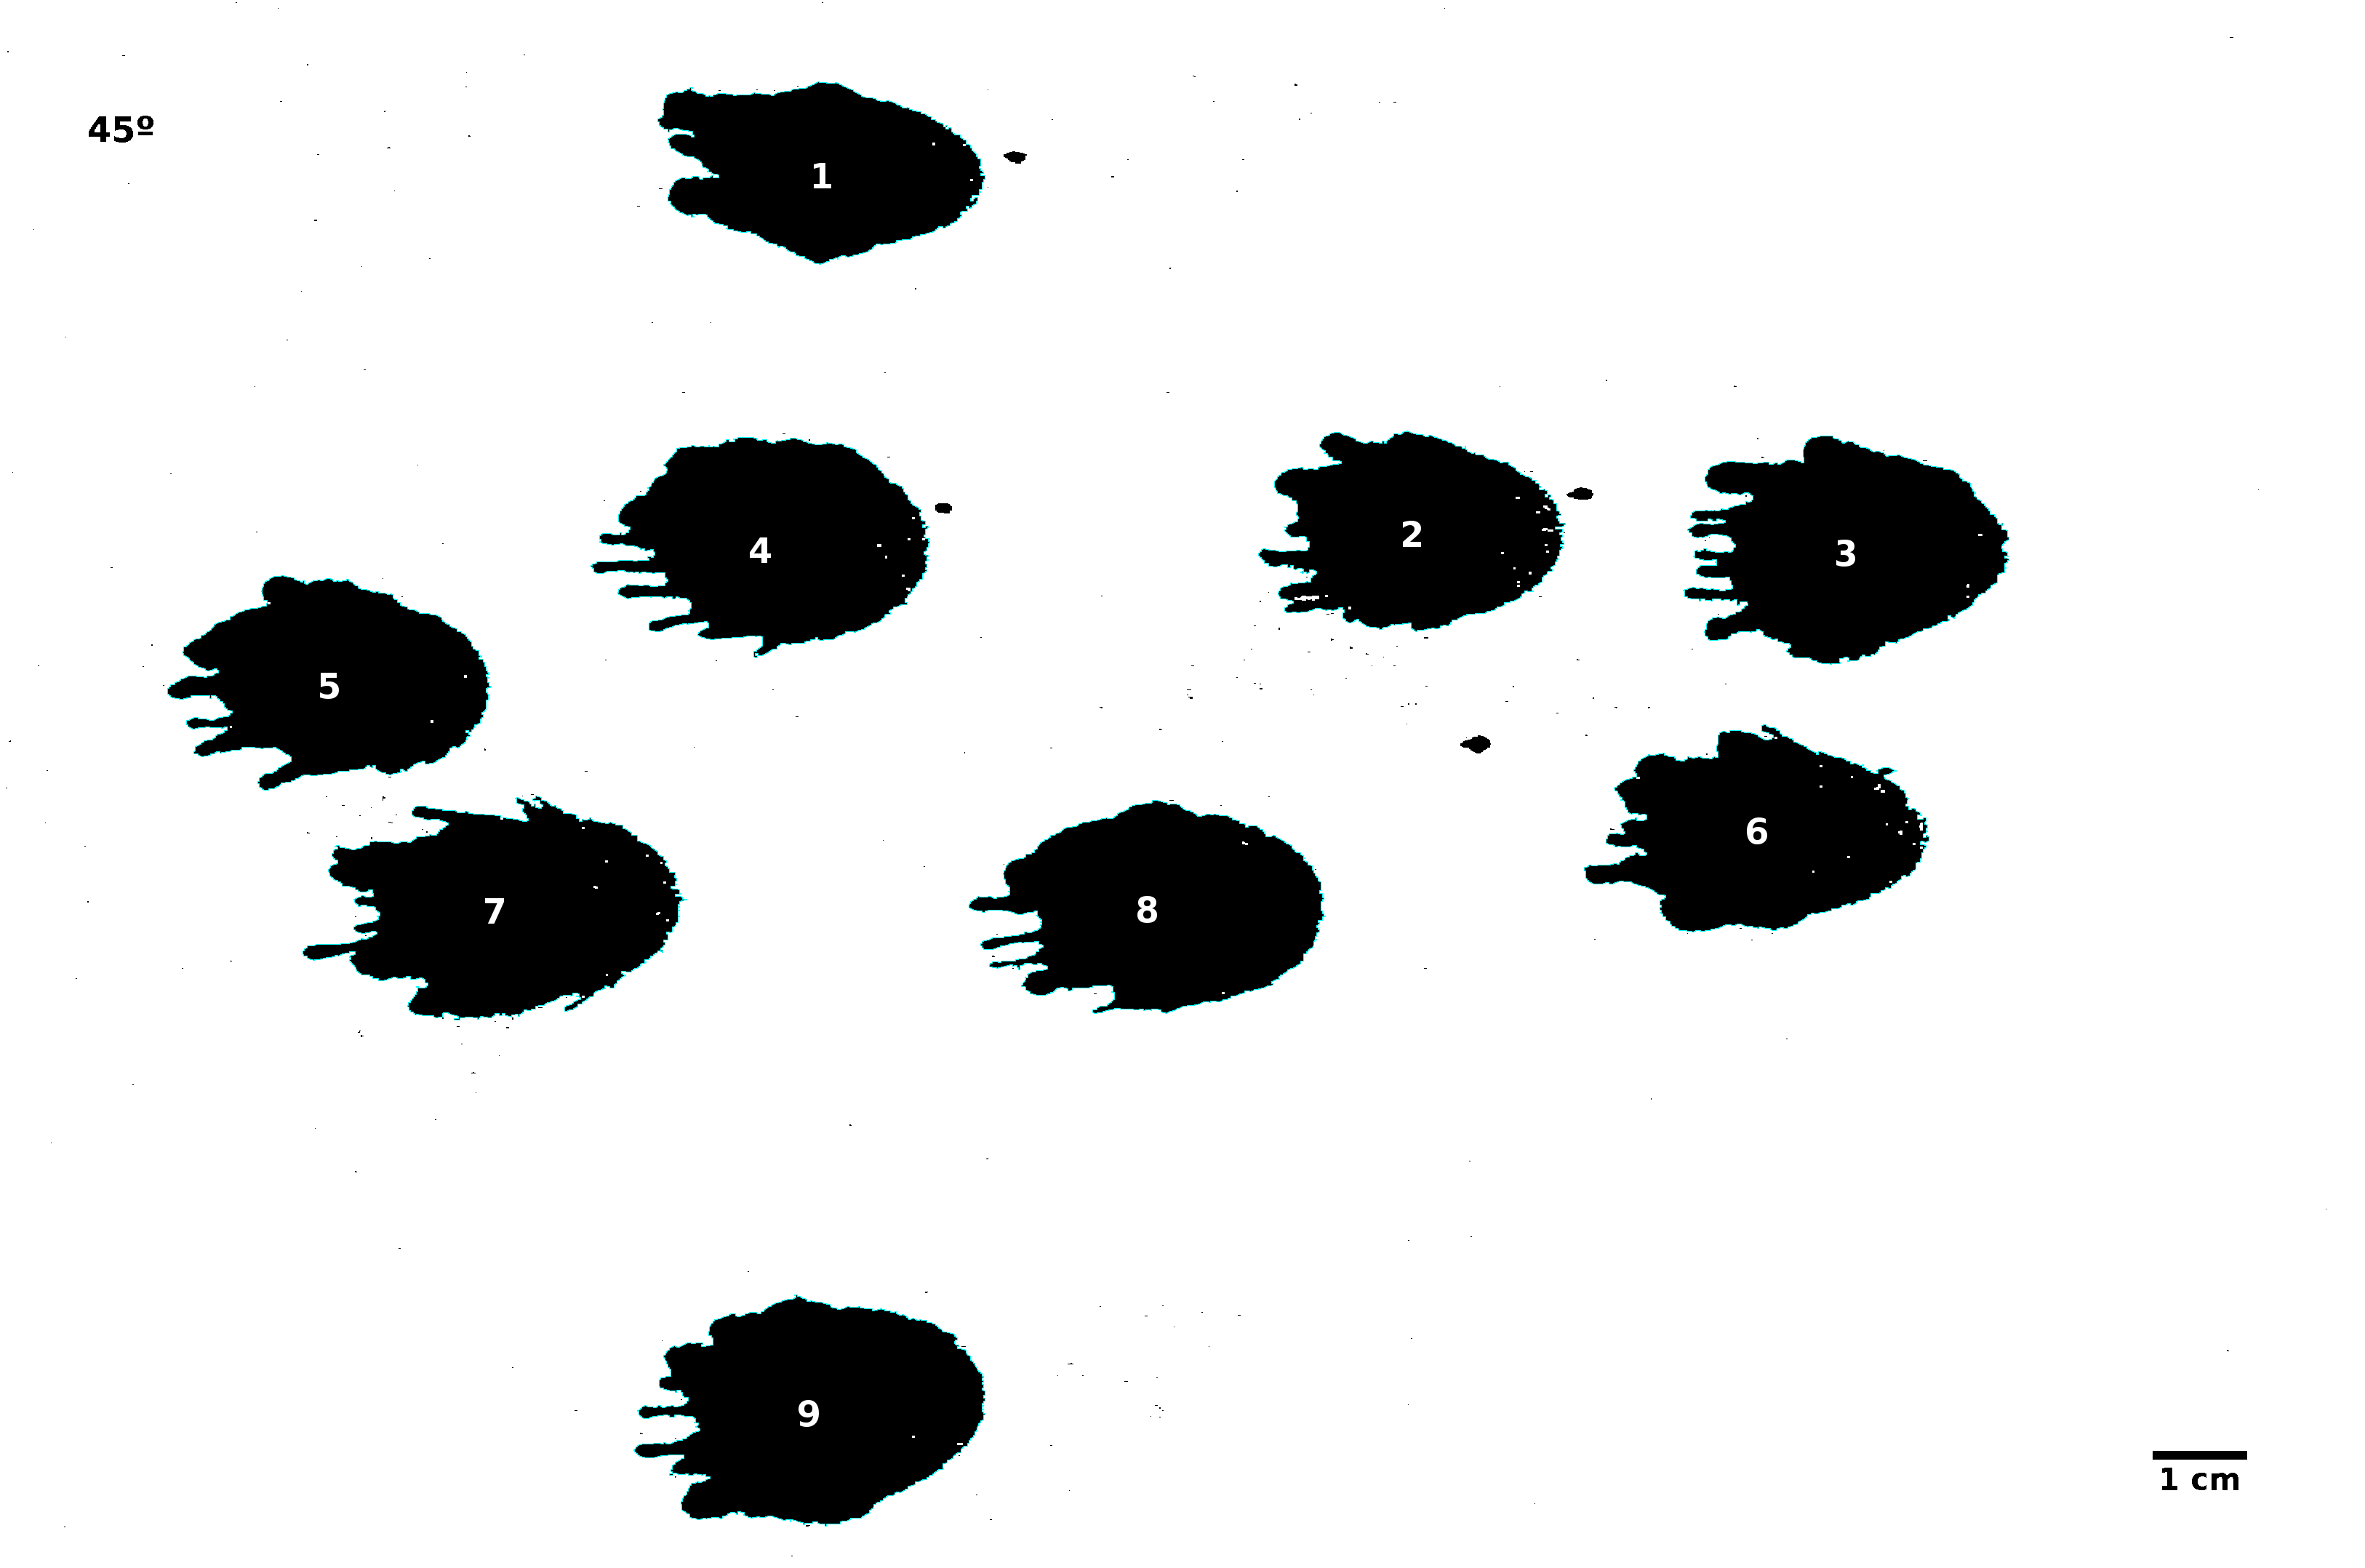
\includegraphics[width=0.66\linewidth]{src/45_deg-1.png} \caption{Mancha de
gotas sobre plano inclinado $45^o$} \label{fig:45deg-1} \end{figure}

\pagebreak

\begin{table}[H] \centering \caption{Datos obtenidos a partir de la figura
    ~\ref{fig:60deg-1} ($\alpha=60^o)$} \label{tab:60deg-1}
    \begin{tabular}{cccccc} \toprule Gota & Área ($cm^2$) & Perímetro ($cm$) &
        Eje mayor ($cm$) & Eje menor ($cm$) & Dirección ($^o$) \\ \midrule 1 &
        8.08 & 21.75 & 8.73 & 1.18 & 0.95   \\ 2 & 5.6  & 18.08 & 6.1  & 1.17 &
        171.92 \\ 3 & 8.4  & 16.42 & 6.46 & 1.66 & 178.11 \\ 4 & 6.69 & 17.99 &
        6.27 & 1.36 & 176.16 \\ 5 & 6.91 & 20.11 & 5.66 & 1.55 & 0.52  \\
    \bottomrule \end{tabular} \end{table}

\begin{figure}[H] \begin{minipage}{.5\textwidth} \centering
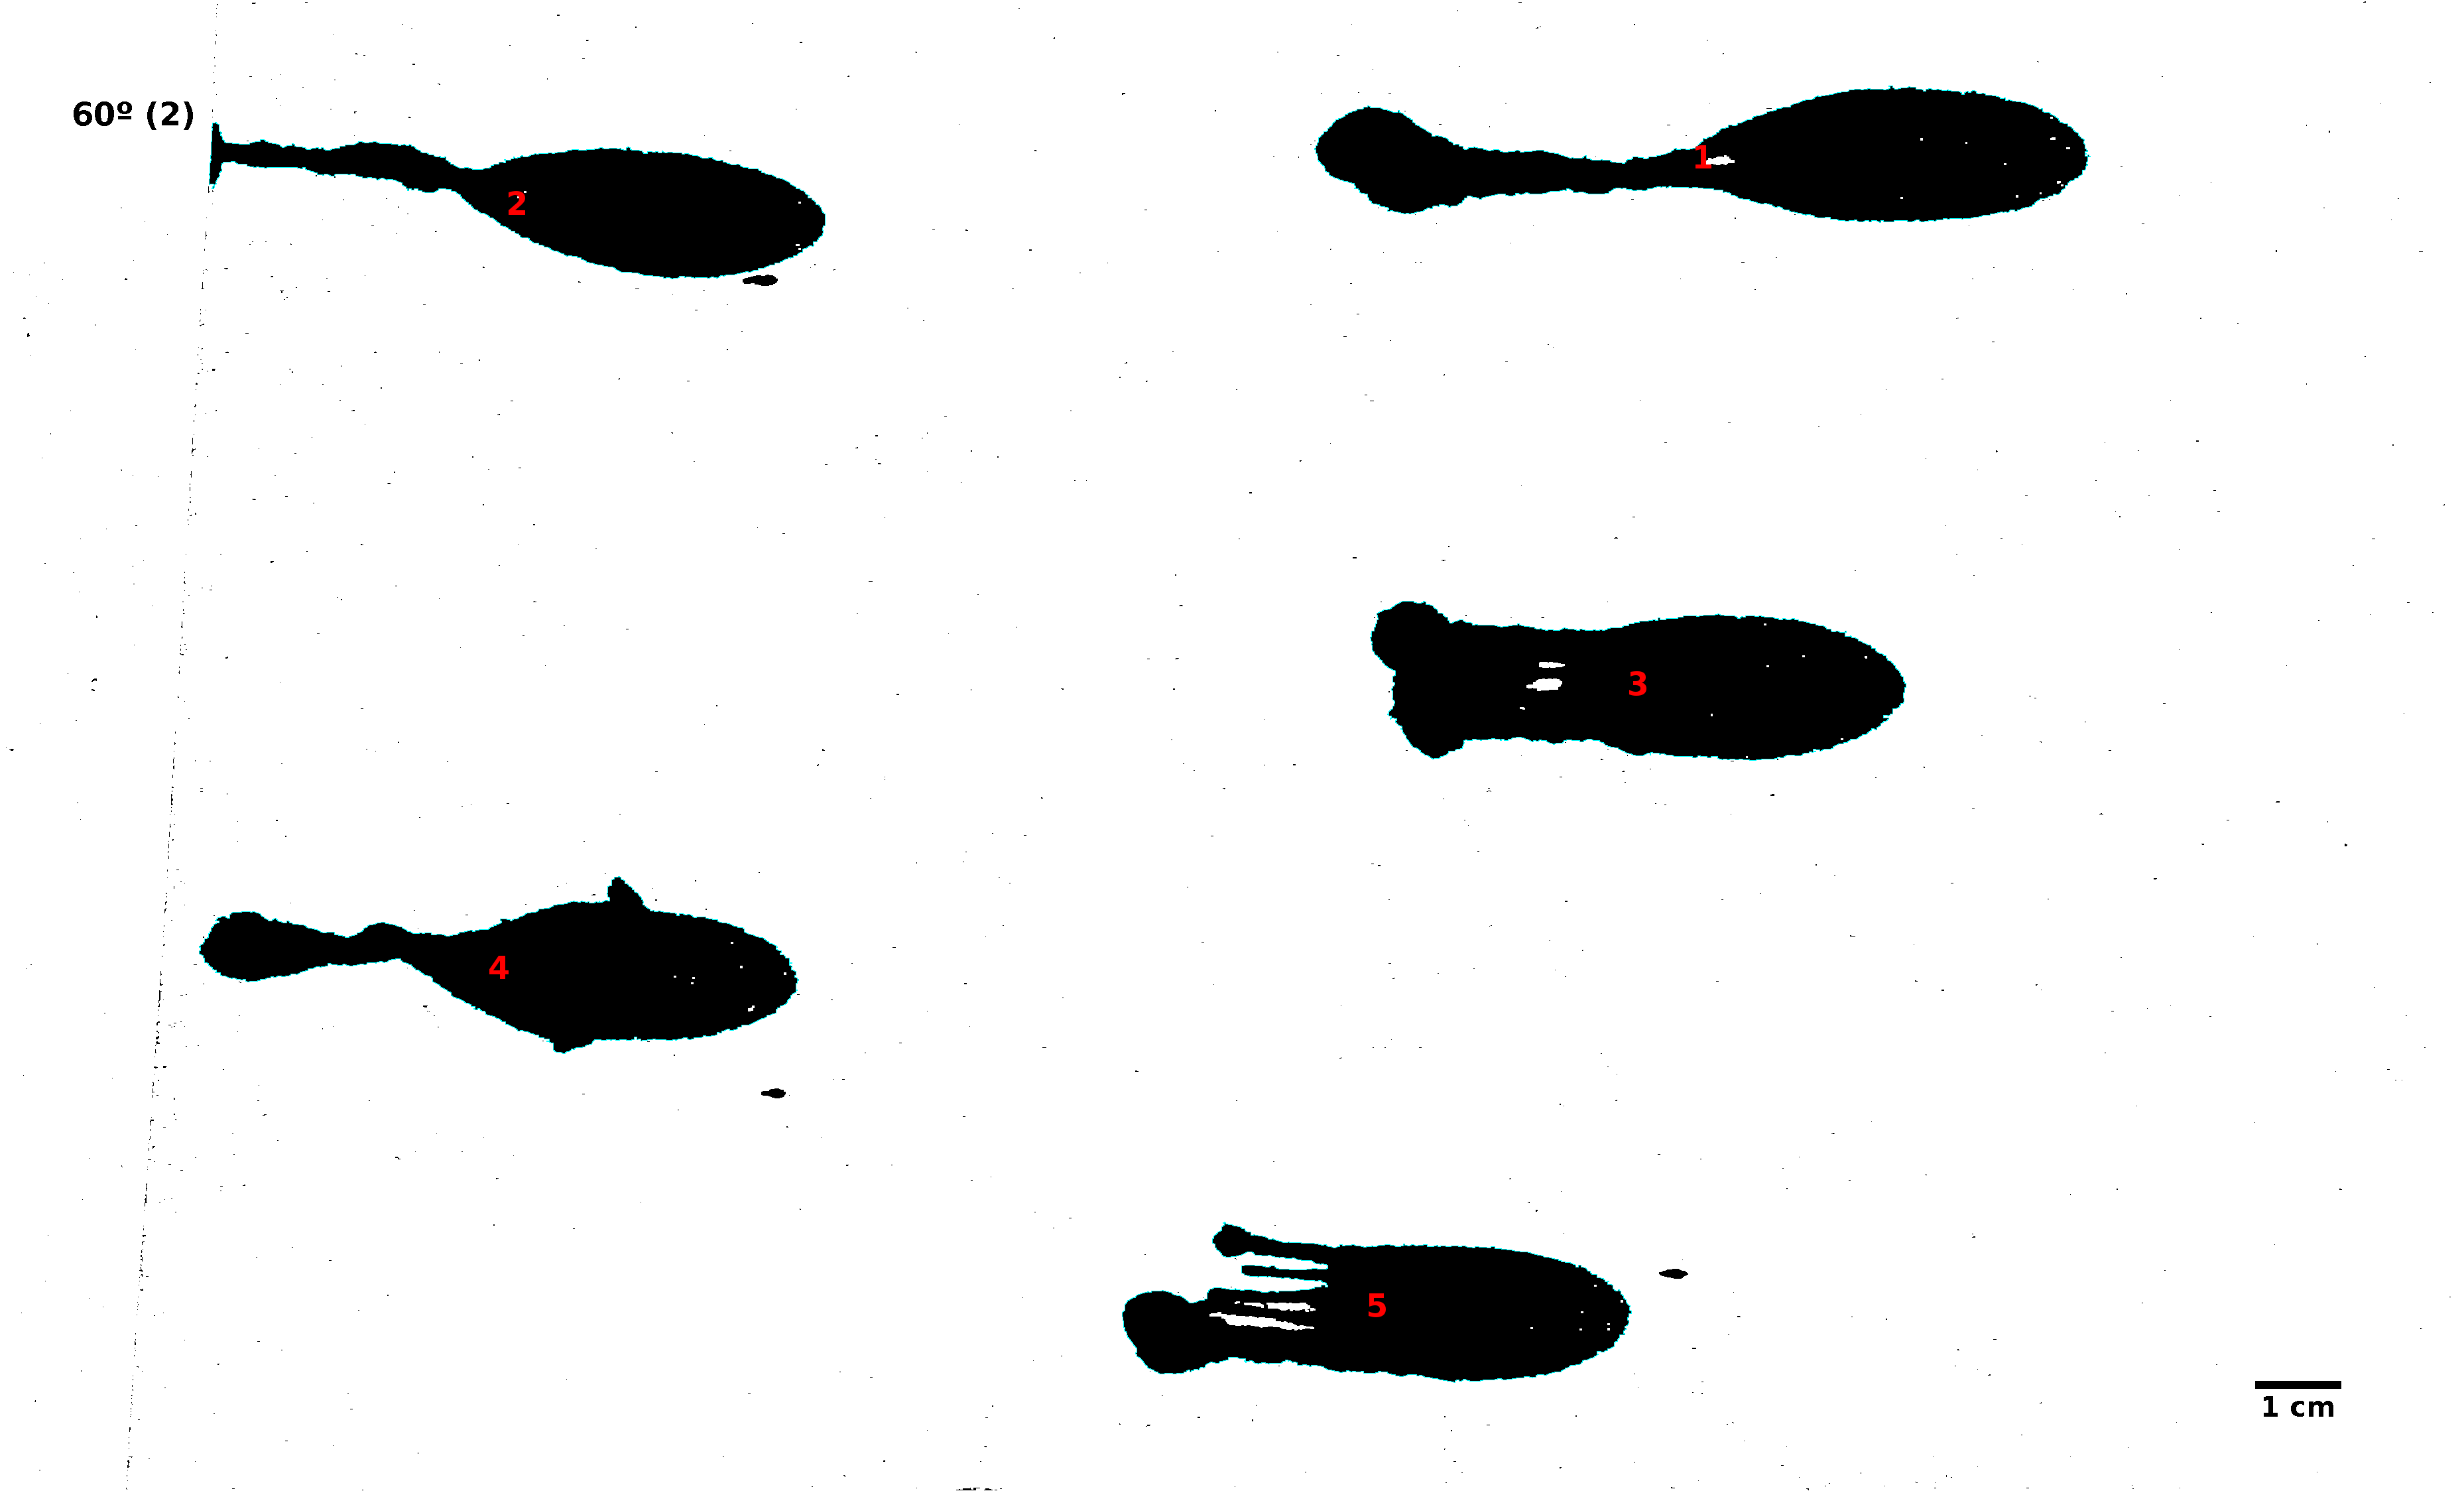
\includegraphics[width=1.0\linewidth]{src/60_deg-1.png} \caption{Mancha de
gotas sobre plano inclinado $60^o$} \label{fig:60deg-1} \end{minipage}%
\begin{minipage}{.5\textwidth} \centering
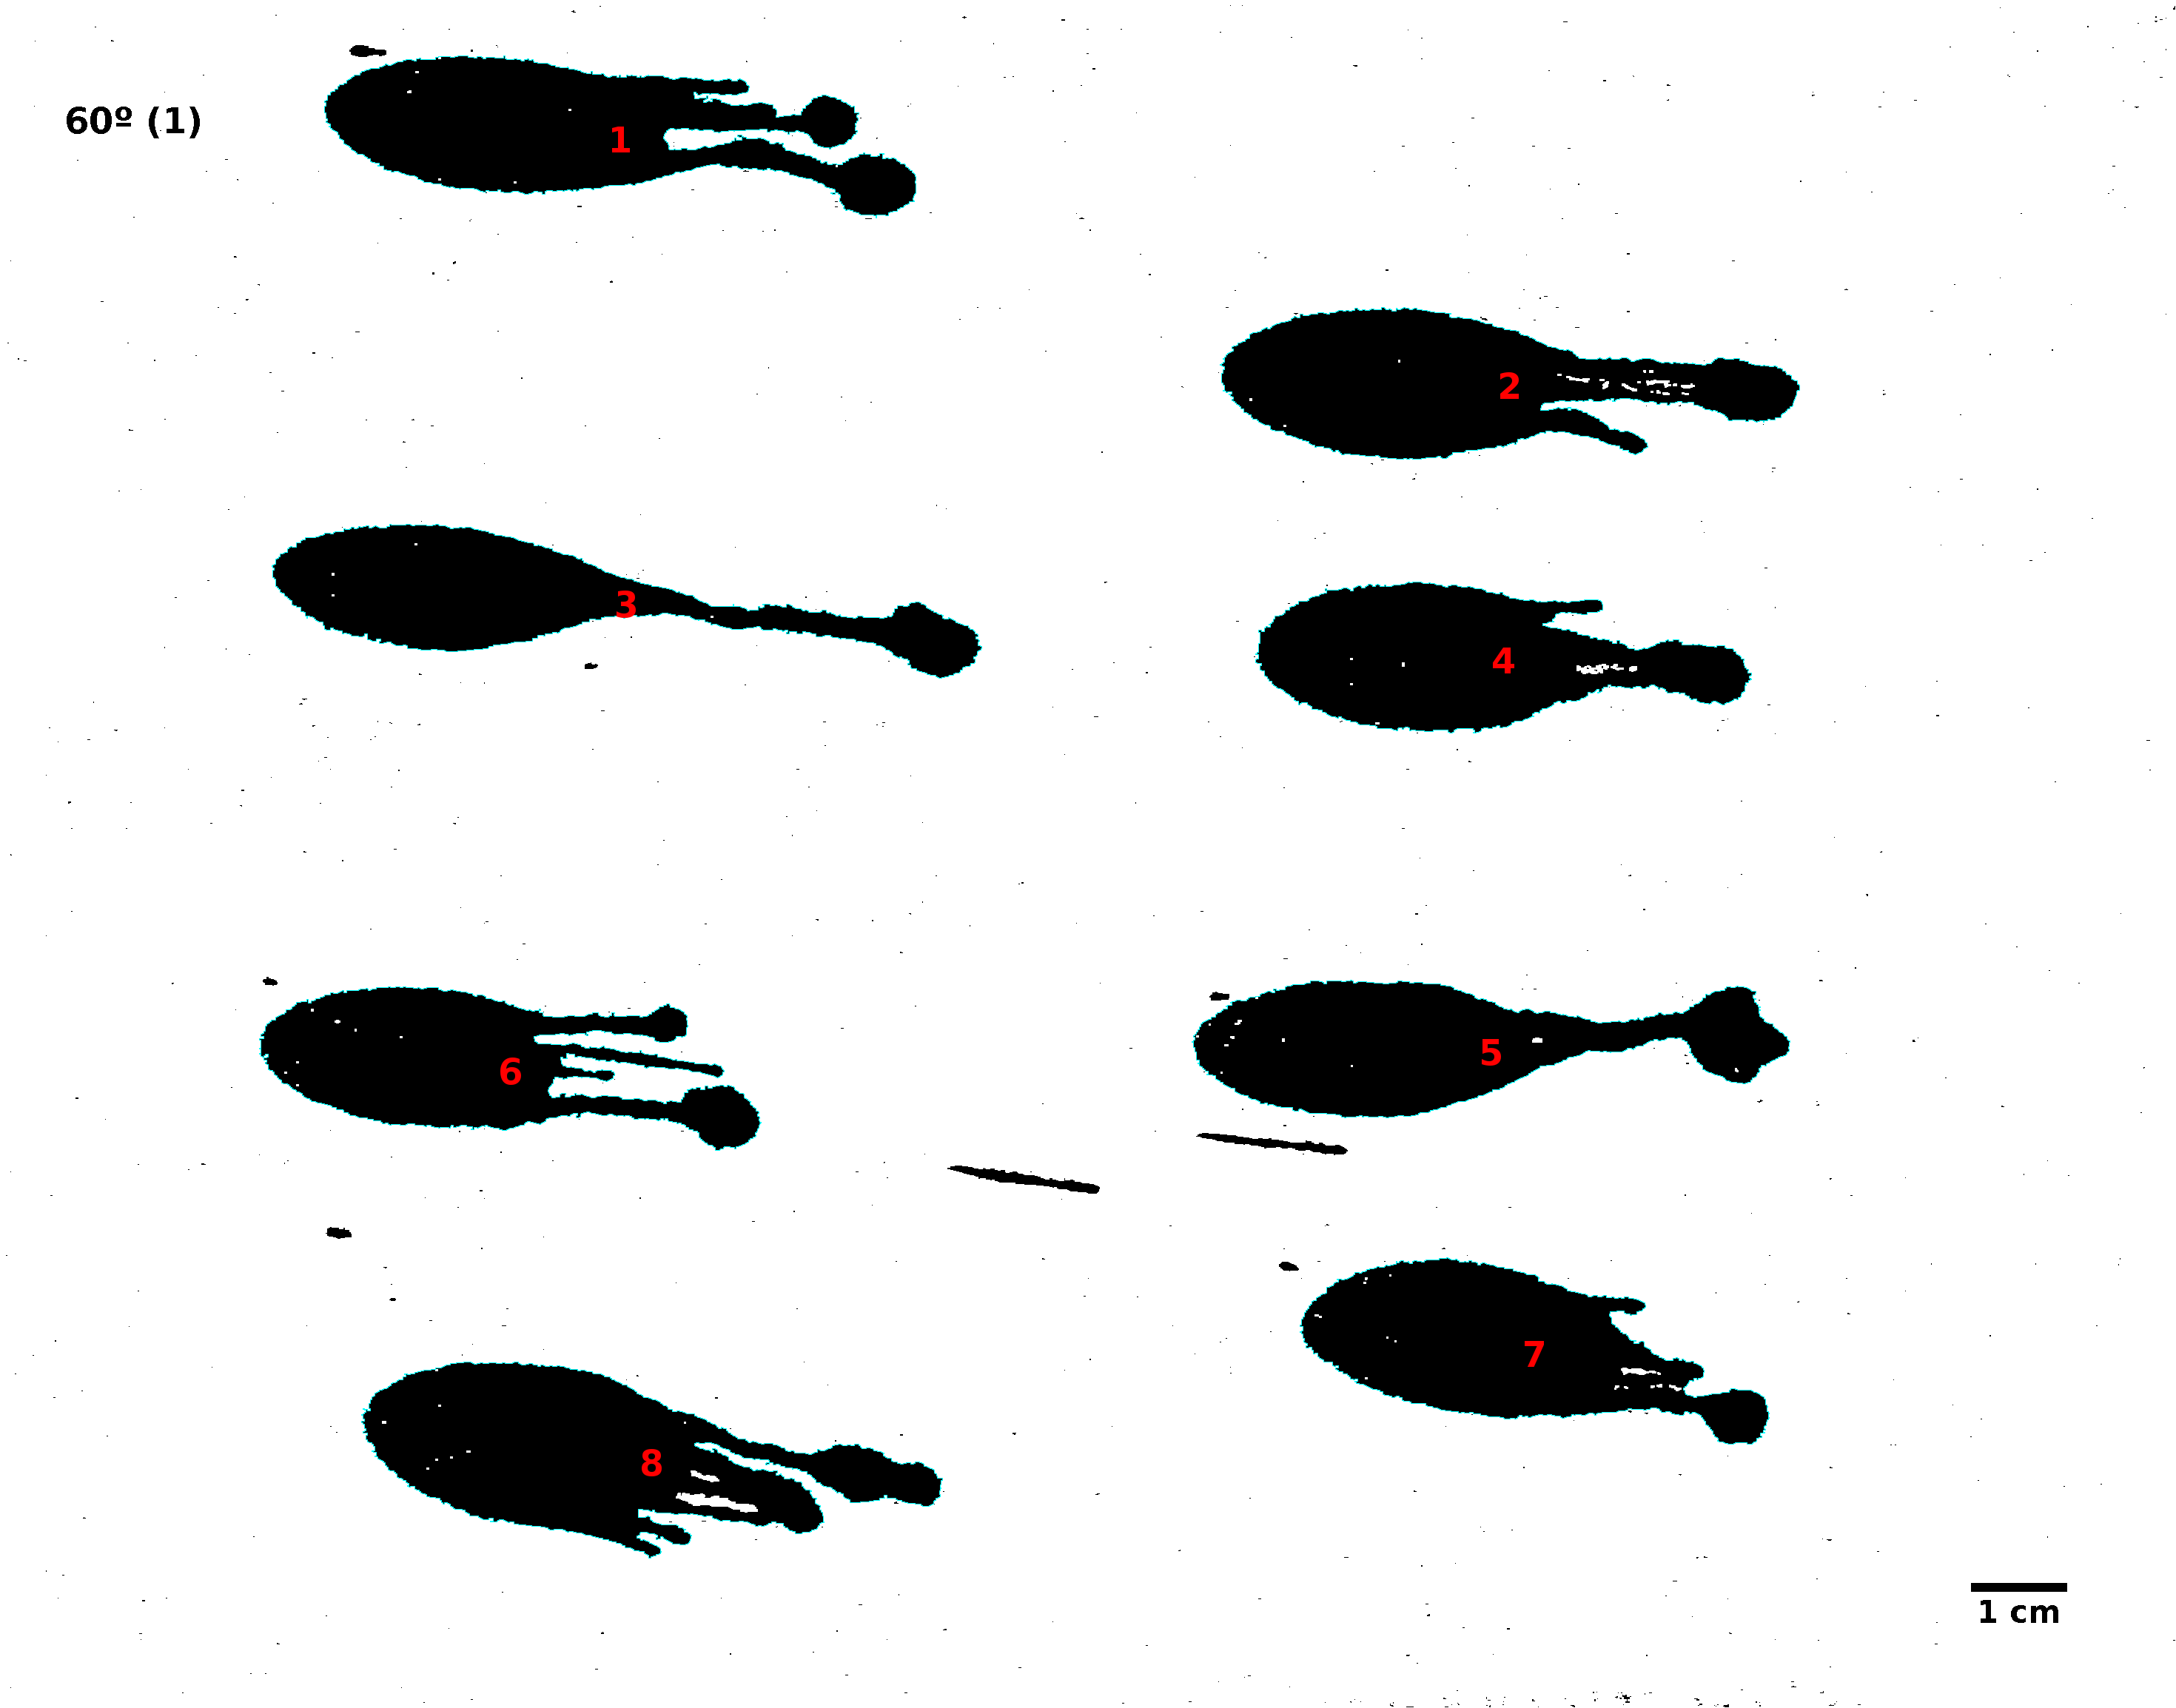
\includegraphics[width=1.0\linewidth]{src/60_2_deg-1.png} \caption{Mancha de
gotas sobre plano inclinado $60^o$} \label{fig:60deg-2} \end{minipage}

\end{figure}

\begin{table}[H] \centering \caption{Datos obtenidos a partir de la figura
    ~\ref{fig:60deg-2} ($\alpha=60^o)$} \label{tab:60deg-2}
    \begin{tabular}{cccccc} \toprule Gota & Área ($cm^2$) & Perímetro ($cm$) &
        Eje mayor ($cm$) & Eje menor ($cm$) & Dirección ($^o$) \\ \midrule 1 &
        5.72 & 22.26 & 5.8  & 1.26 & 175.06 \\ 2 & 5.64 & 17.55 & 5.46 & 1.32 &
        178.16 \\ 3 & 4.72 & 18.09 & 6.55 & 0.92 & 174.27 \\ 4 & 5.02 & 14.86 &
        4.7  & 1.36 & 177.54 \\ 5 & 5.21 & 15.65 & 5.78 & 1.15 & 1.8    \\ 6 &
        4.86 & 23.01 & 4.68 & 1.32 & 173.55 \\ 7 & 5.06 & 14.38 & 4.46 & 1.44 &
        168.08 \\ 8 & 6.35 & 21.21 & 5.36 & 1.51 & 172.24 \\ \midrule Media
        \footnotemark & 6.02 &	18.57 &	5.85 &	1.32 &	134.49 \\ \bottomrule
    \end{tabular} \end{table} \footnotetext{La media corresponde a los datos de
    las tablas \ref{tab:60deg-1} y \ref{tab:60deg-2}}

\begin{table}[H] \centering \caption{Datos obtenidos a partir de la figura
    ~\ref{fig:75deg-1} ($\alpha=75^o)$} \label{tab:75deg-1}
    \begin{tabular}{cccccc} \toprule Gota & Área ($cm^2$) & Perímetro ($cm$) &
        Eje mayor ($cm$) & Eje menor ($cm$) & Dirección ($^o$) \\ \midrule 1 &
        6.13 & 23.99 & 9.32 & 0.84 & 176.54 \\ 2 & 5.18 & 22.29 & 9.02 & 0.73 &
        177.15 \\ 3 & 5.6  & 24.89 & 9.6  & 0.74 & 174.7  \\ 4 & 3.41 & 19.42 &
        8.13 & 0.53 & 179.57 \\ \bottomrule \end{tabular} \end{table}

\begin{figure}[H] \begin{minipage}{.5\textwidth} \centering
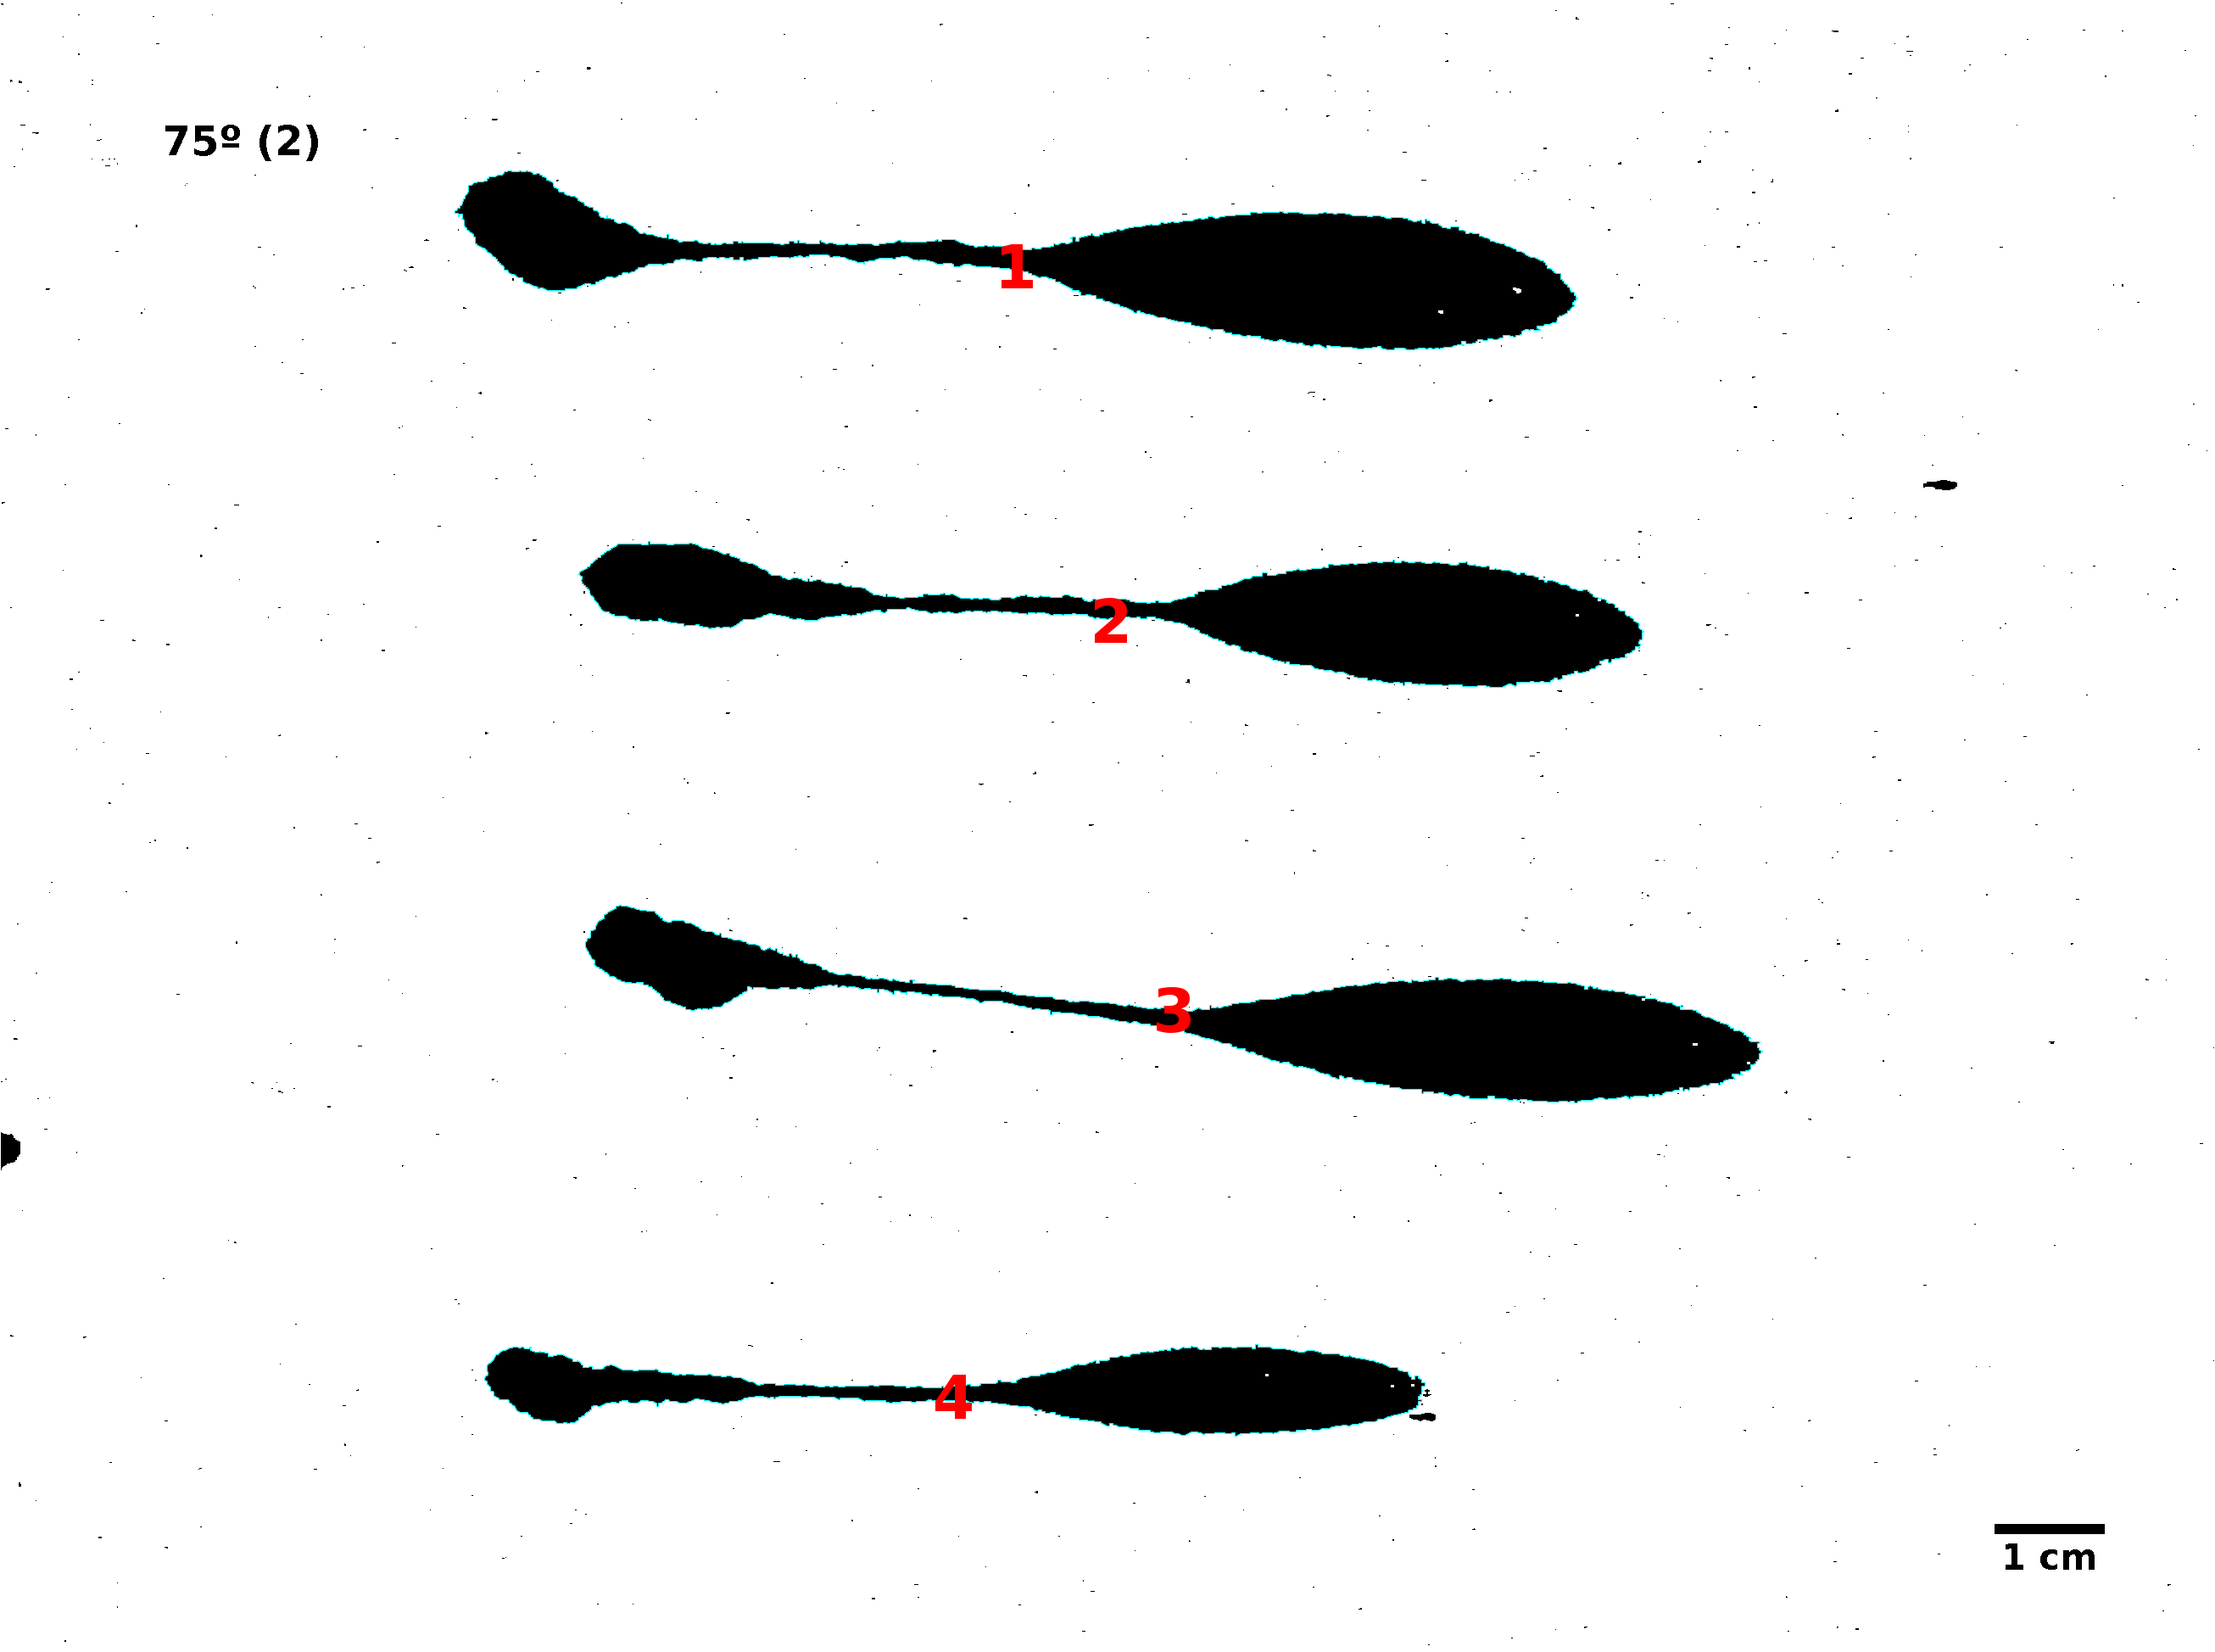
\includegraphics[width=1.0\linewidth]{src/75_deg-1.png} \caption{Mancha de
gotas sobre plano inclinado $75^o$} \label{fig:75deg-1} \end{minipage}%
\begin{minipage}{.5\textwidth} \centering
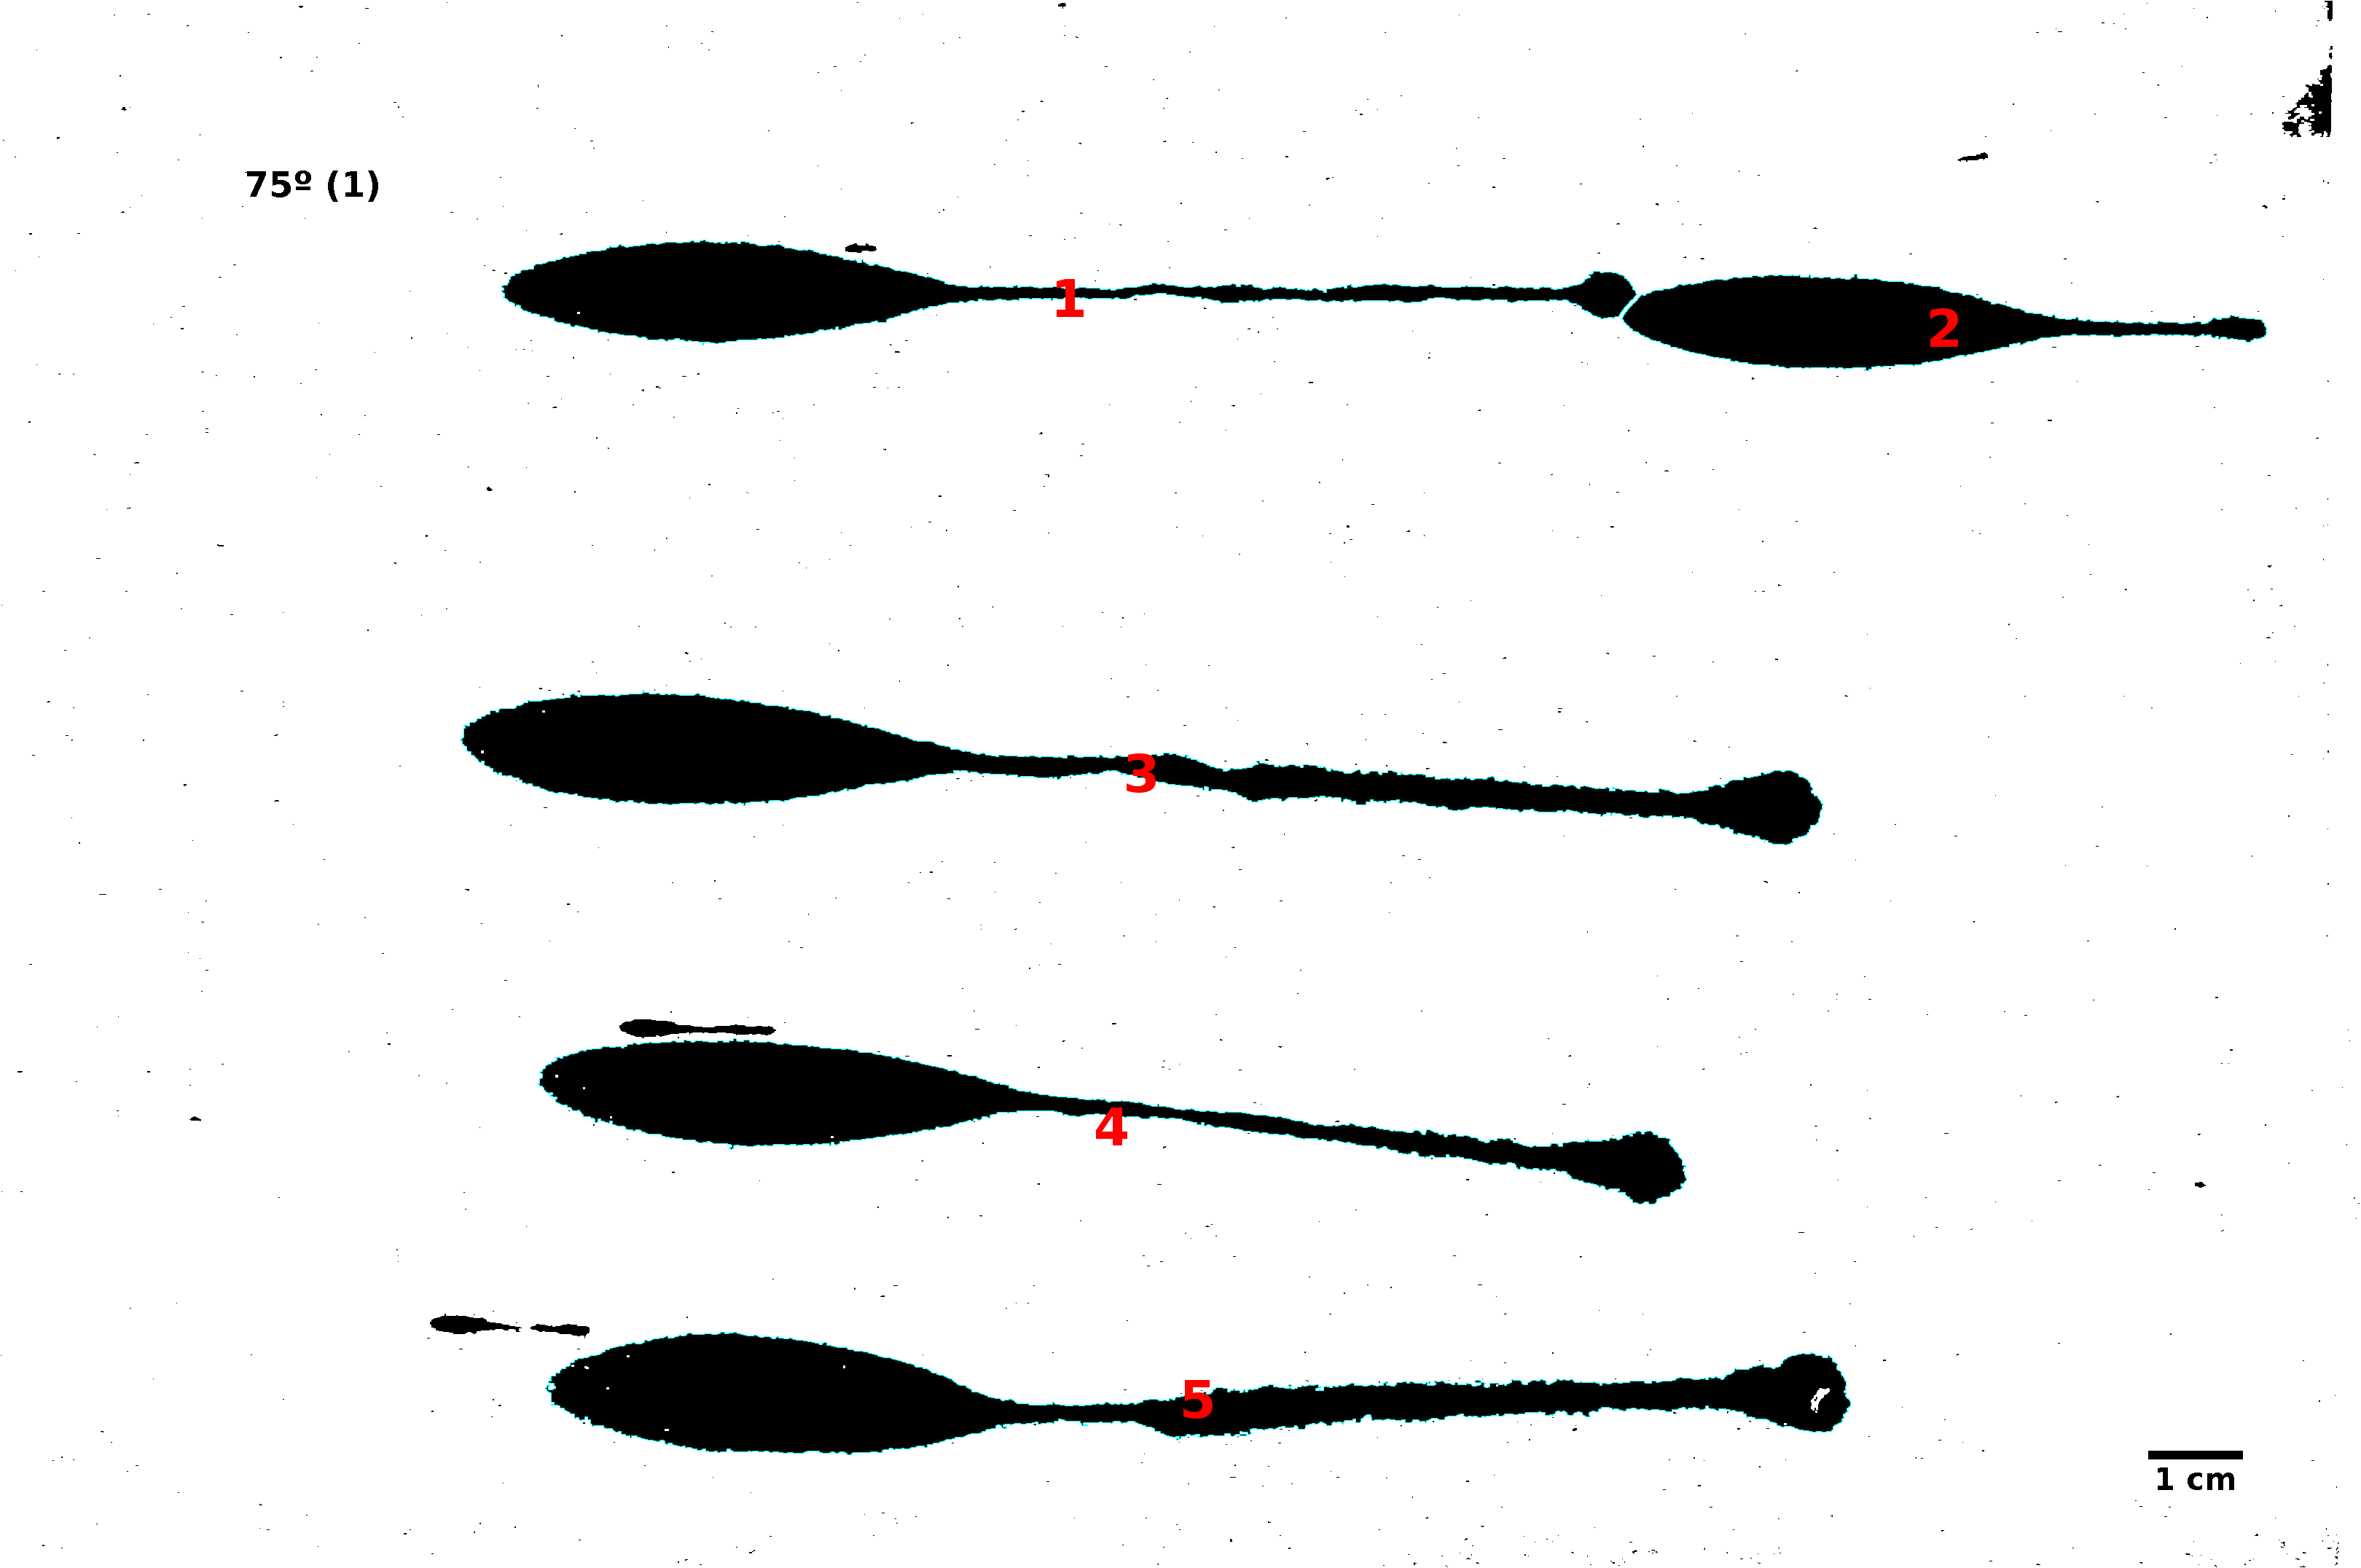
\includegraphics[width=1.0\linewidth]{src/75_2_deg-1.png} \caption{Mancha de
gotas sobre plano inclinado $75^o$} \label{fig:75deg-2} \end{minipage}

\end{figure}

\begin{table}[H] \centering \caption{Datos obtenidos a partir de la figura
    ~\ref{fig:75deg-2} ($\alpha=75^o)$} \label{tab:75deg-2}
    \begin{tabular}{cccccc} \toprule Gota & Área ($cm^2$) & Perímetro ($cm$) &
        Eje mayor ($cm$) & Eje menor ($cm$) & Dirección ($^o$) \\ \midrule 1 &
        4.69 & 27.02 & 9.17  & 0.65 & 179.8  \\ 2 & 3.62 & 15.4  & 5.55  & 0.83
             & 178.68 \\ 3 & 7.24 & 33.79 & 13.19 & 0.7  & 176.94 \\ 4 & 5.86 &
        28.51 & 10.62 & 0.7  & 175.52 \\ 5 & 7.71 & 34.32 & 12.53 & 0.78 &
    179.81 \\ \midrule Media \footnotemark & 5.49 & 25.51 & 9.68 & 0.72 &
177.63 \\ \bottomrule \end{tabular} \end{table} \footnotetext{La media
corresponde a los datos de las tablas \ref{tab:75deg-1} y \ref{tab:75deg-2}}


Las tablas \ref{tab:proc1} y \ref{tab:proc2} muestran
respectivamente la media de los datos obtenidos en cada una de las diferentes
alturas del primer experimento y la media de los datos para cada una de las
inclinaciones del segundo experimento con sus valores de error
correspondientes.

El error corresponde a la suma del error de precisón del instrumento usado y el
error aleatorio siguiendo la formula que se muestra en
\ref{eq:error}\footnote{El error de precisión del área es el mismo que el del
perímetro ya que el programa calcula el área contando píxeles y por lo tanto no
se propaga.}: 
\begin{equation}
\label{eq:error}
E_{total}=
\sqrt{
E_\text{precisón}^2
+E_\text{aleatorio}^2
} 
\end{equation} 
\begin{align}
    E_\text{precisión}&=0.1\ 
    \text{cm} 
    \qquad 
    \text{(Error de la regla usada en las
imágenes)} \\ 
    E_\text{aleatorio} &= \frac{1}{N}*
    \sum_{i=1}^N
    \sqrt{
    \left(v_i -
\overline{v}
\right)^2} 
\qquad 
\text{
(Desviación 
estándar)
} 
\end{align}


\begin{table}[H] \centering \caption{Datos obtenidos en el experimento 1}
    \label{tab:proc1} \begin{tabular}{cccccc} \toprule Altura ($cm$) & Área
        ($cm^2$) & Perímetro ($cm$) & Eje mayor ($cm$) & Eje menor ($cm$) \\
        \midrule $10\pm0.1$  &   1.6 $\pm$ 0.3 &   7.1 $\pm$ 1.2 &   1.5 $\pm$
        0.2 & 1.4 $\pm$ 0.2 \\ $20\pm0.1$  &   2.3 $\pm$ 0.4 &   7.5 $\pm$ 0.9
            &   1.7 $\pm$ 0.2 & 1.7 $\pm$ 0.2 \\ $30\pm0.1$  &   3.1 $\pm$ 0.5
            &   9.2 $\pm$ 1.0 &   2.0 $\pm$ 0.2 & 1.9 $\pm$ 0.2 \\ $40\pm0.1$
            &   3.4 $\pm$ 0.4 &   12.1    $\pm$ 1.7 &   2.1 $\pm$ 0.2 &   2.0
        $\pm$ 0.2 \\ $50\pm0.1$  &   3.5 $\pm$ 0.4 &   11.5    $\pm$ 1.3 &
        2.2 $\pm$ 0.2 &   2.0 $\pm$ 0.1 \\ $60\pm0.1$  &   3.7 $\pm$ 0.4 &
        12.2    $\pm$ 1.2 &   2.2 $\pm$ 0.2 &   2.1 $\pm$ 0.2 \\ $70\pm0.1$  &
        3.8 $\pm$ 0.6 &   13.6    $\pm$ 1.8 &   2.3 $\pm$ 0.2 &   2.1 $\pm$ 0.2
        \\ $80\pm0.1$  &   4.1 $\pm$ 0.3 &   14.7    $\pm$ 1.6 &   2.4 $\pm$
        0.1 &   2.2 $\pm$ 0.1 \\ $90\pm0.1$  &   4.3 $\pm$ 0.4 &   15.6
        $\pm$ 2.0 &   2.4 $\pm$ 0.1 &   2.3 $\pm$ 0.1 \\ $100\pm 0.1$ &   4.7
        $\pm$ 0.7 &   17.7    $\pm$ 1.8 &   2.6 $\pm$ 0.2 &   2.3 $\pm$ 0.2 \\
    \bottomrule \end{tabular} \end{table}

\begin{table}[H] \centering \caption{Datos obtenidos en el experimento 2}
    \label{tab:proc2} \begin{tabular}{cccccc} \toprule Altura ($cm$) & Área
        ($cm^2$) & Perímetro ($cm$) & Eje mayor ($cm$) & Eje menor ($cm$) \\
        \midrule 15	$\pm0.1$ &	4.0	$\pm$	0.7	&	9.80	$\pm$	1.05	&
        2.34	$\pm$	0.24	&	2.17	$\pm$	0.22	\\ 30	$\pm0.1$ &
        4.5	$\pm$	0.6	&	12.43	$\pm$	1.07	&	2.59	$\pm$	0.23
                      &	2.19	$\pm$	0.18	\\ 45	$\pm0.1$ &	5.4	$\pm$
        0.6	&	14.45	$\pm$	1.67	&	3.28	$\pm$	0.20	&	2.09
        $\pm$	0.19	\\ 60	$\pm0.1$ &	6.0	$\pm$	1.2	&	18.57	$\pm$
        2.88	&	5.85	$\pm$	1.10	&	1.32	$\pm$	0.22	\\ 75
    $\pm0.1$ &	5.5	$\pm$	1.5	&	25.51	$\pm$	6.22	&	9.68	$\pm$
2.28	&	0.72	$\pm$	0.14	\\ \bottomrule \end{tabular} \end{table}



\pagebreak \section{Análisis de datos} \label{sec:analisis_de_datos}


\begin{figure}[H] \centering
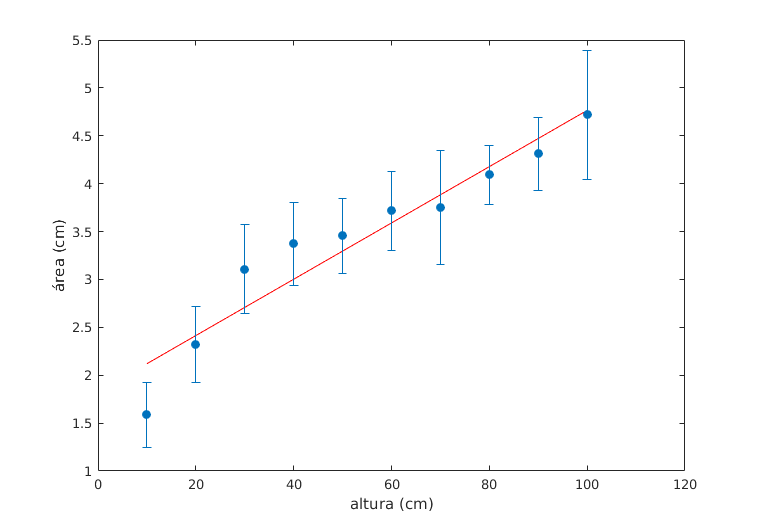
\includegraphics[width=0.9\linewidth]{src/area_vs_height.png} \caption{Área vs.
Altura} \label{fig:area_altura} \end{figure}

\begin{figure}[H] \centering
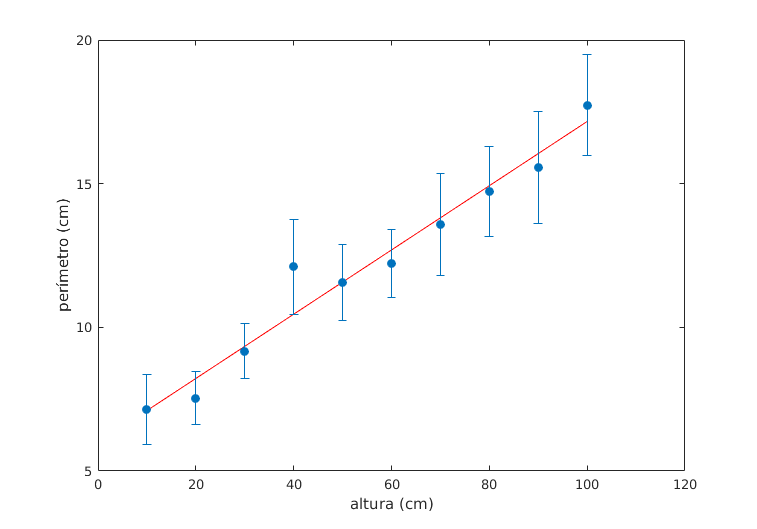
\includegraphics[width=0.9\linewidth]{src/perimeter_vs_height.png}
\caption{Perímetro vs. Altura} \label{fig:perimetro_altura} \end{figure}

La figura \ref{fig:area_altura} muestra la correlación entre el área y la
altura desde que se lanzó la gota. Esta relación tiene un comportamiento lineal
descrito por la función \ref{eq:fit_a_h}: \begin{align}\label{eq:fit_a_h} A(h)
    &= a*h + b \\ a &= 0.02939 \pm 0.00743 \nonumber \\ b &= 1.826 \pm 0.461
\nonumber \end{align}

La figura \ref{fig:perimetro_altura} muestra la correlación entre el perímetro
y la altura desde que se lanzó la gota. Esta relación tiene un comportamiento
lineal descrito por la función \ref{eq:fit_p_h}:
\begin{align}\label{eq:fit_p_h} P(h) &= a*h + b \\ a &= 0.1118 \pm 0.0181
\nonumber \\ b &= 5.984 \pm 1.125 \nonumber \end{align}

\subsection{Observaciones}

Podemos observar que la pendiente de la función que modeliza el área es menor a
la del perímetro, por consiguiente, el perímetro aumenta mucho más rápido que
el área en relación a la altura, debido a los "picos" que se forman al caer de
mayor altura. 



\begin{figure}[H] \centering
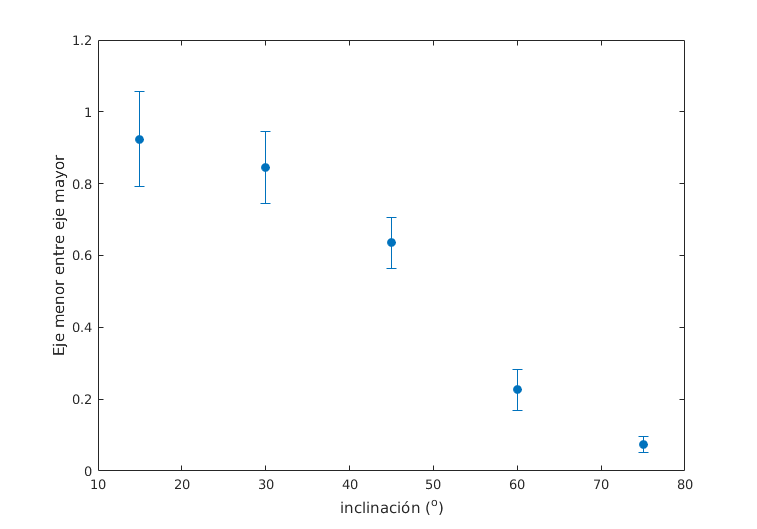
\includegraphics[width=0.9\linewidth]{src/ejes_vsheight.png}
\caption{Proporción eje mayor - eje menor respecto a la inclinación del plano
de impacto} \label{fig:ejes_inclinacion} \end{figure}



\section{Evaluación de los resultados} \label{sec:evaluacion}







\section{Conclusión} \label{sec:conclusion}


\pagebreak \printbibliography[heading=bibintoc,title={Bibliografía}]

\end{document}
